%\documentclass[handout,dvipsnames,12pt]{beamer} % for the version to send to students
\documentclass[dvipsnames,aspectratio=169]{beamer} % for the version with visual breaks
\usepackage{tikz,xcolor,amsfonts}
\usetikzlibrary{arrows,shapes}
\usepackage[absolute,overlay]{textpos}
\usepackage{multirow}
\usepackage{environ,lipsum}
\usepackage{listings}



\lstset{ 
  language=R,                     % the language of the code
  basicstyle=\scriptsize\ttfamily, % the size of the fonts that are used for the code
  columns=fullflexible,
%  numbers=left,                   % where to put the line-numbers
%  numberstyle=\tiny\color{Blue},  % the style that is used for the line-numbers
%  stepnumber=1,                   % the step between two line-numbers. If it is 1, each line
                                  % will be numbered
%  numbersep=5pt,                  % how far the line-numbers are from the code
  backgroundcolor=\color{Dandelion!15!white},  % choose the background color. You must add \usepackage{color}
  showspaces=false,               % show spaces adding particular underscores
  showstringspaces=false,         % underline spaces within strings
  showtabs=false,                 % show tabs within strings adding particular underscores
  frame=single,                   % adds a frame around the code
  rulecolor=\color{Dandelion!15!white},        % if not set, the frame-color may be changed on line-breaks within not-black text (e.g. commens (green here))
  tabsize=2,                      % sets default tabsize to 2 spaces
  captionpos=b,                   % sets the caption-position to bottom
  breaklines=true,                % sets automatic line breaking
  breakatwhitespace=false,        % sets if automatic breaks should only happen at whitespace
  keywordstyle=\color{RoyalBlue!80!black},      % keyword style
  commentstyle=\color{YellowGreen!60!black},   % comment style
  %stringstyle=\color{ForestGreen}      % string literal style
} 
\lstset{alsoletter={.,_}, morekeywords={cor.test,set.seed,dcor.test,make_tree,sample_gnm,graph,ci.test,qgraph,sample_smallworld,ciTest_table,IsingFit,averageLayout,read.table,install.packages,bdgraph,stepwise,dmod,cmod,ciTest,graph_from_adjacency_matrix,mvrnorm,CondIndTest,as.data.frame,chisq.test,gnm,smallworld,ug,dag,edge,as.igraph,degree,diameter,centrality,cluster,betweenness,at}
}


\newcommand{\customframefont}[1]{
\setbeamertemplate{itemize/enumerate body begin}{#1}
\setbeamertemplate{itemize/enumerate subbody begin}{#1}
}

\NewEnviron{framefont}[1]{
\customframefont{#1} % for itemize/enumerate
{#1 % For the text outside itemize/enumerate
\BODY
}
\customframefont{\normalsize}
}



%%%%%%%%% BASICS
\usenavigationsymbolstemplate{}

\setbeamertemplate{frametitle}
  {\begin{centering}\smallskip
   \insertframetitle\par
   \smallskip\end{centering}}
\setbeamersize{text margin left=.2cm,text margin right=.2cm} 
\setbeamertemplate{itemize item}{$\bullet$}
\setbeamertemplate{navigation symbols}{}
\setbeamertemplate{footline}[text line]{%
    \hfill\strut{%
        \scriptsize\sf\color{black!60}%
        \quad\insertframenumber/\inserttotalframenumber
    }%
    \hfill
    
}

%%%%%%%%% COLOR THEME

% Define some colors:
\definecolor{DarkFern}{HTML}{407428}
\definecolor{DarkCharcoal}{HTML}{4D4944}
\colorlet{Fern}{DarkFern!85!white}
\colorlet{Charcoal}{DarkCharcoal!85!white}
\colorlet{LightCharcoal}{Charcoal!50!white}
\definecolor{Important}{RGB}{234,122,133}
\colorlet{AlertColor}{Melon!30!red}
\colorlet{DarkRed}{red!70!black}
\colorlet{DarkBlue}{blue!70!black}
\colorlet{DarkGreen}{green!70!black}
% Use the colors:
\setbeamercolor{title}{fg=Fern}
\setbeamercolor{frametitle}{fg=Fern}
\setbeamercolor{normal text}{fg=Charcoal}
\setbeamercolor{block title}{fg=black,bg=Fern!15!white}
\setbeamercolor{block body}{fg=black,bg=Fern!15!white}
%\setbeamercolor{block body alerted}{fg=black,bg=Goldenrod!5!white}
%\setbeamercolor{block body example}{fg=black,bg=Fern!15!white}
\setbeamercolor{alerted text}{fg=AlertColor}
\setbeamercolor{itemize item}{fg=Charcoal}
\setbeamercolor{framesource}{fg=gray}
\setbeamerfont{framesource}{size=\tiny}

%%%%% DEFINITIONS

\DeclareMathOperator{\sgn}{sgn}
\DeclareMathOperator{\rank}{rank}
\DeclareMathOperator{\D}{D}
\DeclareMathOperator{\cov}{cov}
\DeclareMathOperator{\var}{var}
\DeclareMathOperator{\tr}{tr}
\DeclareMathOperator{\pa}{pa}
\DeclareMathOperator{\nd}{nd}

\newcommand{\bx}{\mathbf{x}}
\newcommand{\by}{\mathbf{y}}
\newcommand{\C}{\mathbb{C}}
\newcommand{\cC}{\mathcal{C}}
\newcommand{\E}{\mathbb{E}}
\newcommand{\cE}{\mathcal{E}}
\newcommand{\cI}{\mathcal{I}}
\newcommand{\J}{\rm {J}}
\newcommand{\cL}{\mathcal{L}}
\newcommand{\cM}{\mathcal{M}}
\newcommand{\N}{\mathbb{N}}
\renewcommand{\P}{\mathbb{P}}
\newcommand{\Q}{\mathbb{Q}}
\newcommand{\R}{\mathbb{R}}
\renewcommand{\S}{\mathbb{S}}
\newcommand{\cS}{\mathcal{S}}
\newcommand{\cX}{\mathcal{X}}
\newcommand{\Z}{\mathbb{Z}}
\newcommand{\bs}{\boldsymbol}
\newcommand{\why}{\textcolor{WildStrawberry}{{\textsc{why?}}}}
\newcommand{\indep}{\mbox{\,$\perp\!\!\!\perp$\,}}
\newcommand{\mtp}{{\rm MTP}_{2}}


\def\imagetop#1{\vtop{\null\hbox{#1}}}
\def\house{\hbox{\kern3pt \vbox to12pt{}% 
   \pdfliteral{q 0 0 m 0 5 l 5 10 l 10 5 l 10 0 l 7 0 l 7 5 l 3 5 l 3 0 l f
               1 j 1 J -2 5 m 5 12 l 12 5 l S Q }%
   \kern 13pt}}

%source for images
\newcommand{\source}[1]{\begin{textblock*}{4cm}(8.7cm,8.6cm)
    \begin{beamercolorbox}[ht=0.5cm,right]{framesource}
        \usebeamerfont{framesource}\usebeamercolor[fg]{framesource} Source: {#1}
    \end{beamercolorbox}
\end{textblock*}}

%%% TITLE INFO

\title{Advanced techniques in applied economics}
\subtitle{Modelling with graphs, Lectures 1-5}

\author{Piotr Zwiernik}

\institute{\begin{center}
  \raisebox{-0.5\height}{
\includegraphics[scale=.27]{LOGOstats.png}}
  \hspace{1mm}
  \raisebox{-0.5\height}{
\includegraphics[scale=.08]{LOGOBSE.jpg}}
\end{center}}


\setbeamercolor{notabene}{fg=black!50!white,bg=Gray!10!white}
\setbeamercolor{important}{fg=red!50!white,bg=red!7!white}
\setbeamercolor{goldbox}{fg=black!50!white,bg=Goldenrod!7!white}
\setbeamercolor{result}{fg=black!60!white,bg=OliveGreen!4!white}
% \begin{beamercolorbox}[wd=\paperwidth,sep=7pt]{important}	
%	%\end{beamercolorbox}


\begin{document}

%\addtocounter{framenumber}{-1}
\begin{frame}[noframenumbering,plain]
  \titlepage
\end{frame}

\section{About the course}
\begin{frame}[plain,noframenumbering]{}
\begin{center}
	{\huge \textcolor{DarkRed}{About the course}}
\end{center}
\end{frame}



\begin{frame}{Modeling with graphs - Outline}
Discuss three important concepts in data modelling.\\[.2cm] 
\begin{enumerate}
	     \item Conditional independence. \\[.3cm] 
		\item Causality.\\[.3cm] 
		\item Positive dependence.\\[.8cm] 
	\end{enumerate}
	
	All discussed in the context of \alert{modelling with graphs and networks}.\\[.6cm]
	The course will be kept high level. It is designed as an invitation to graphical modelling. 
	
%	The course will be kept high level.\\[.4cm]
%	We will work with explicit examples (in \textsc{R})
\end{frame}

\begin{frame}{Literature}
	The literature on graphical models and causality is rich.\\[.4cm]
	I find the following books particularly useful for this course:\\[.2cm]
	\begin{enumerate}
		\item S.~H{\o}jsgaard, D.~Edwards, S.~Lauritzen, \emph{Graphical models in \textsc{R}}\\[.3cm]
		\item J.~Peters, D.~Janzing, B.~Sch\"{o}lkopf, \emph{Elements of Causal Inference}. (mainly Chapters 6 and 7)\\[.3cm]
		\item \emph{Handbook of Graphical models}, edited by M.~Maathuis, M.~Drton, S.~Lauritzen, M.~Wainwright. (mainly Chapters 12-15 and 18)
	\end{enumerate}
	\bigskip
	To present state-of-the-art methods I will rely also on recent articles.
\end{frame}

\begin{frame}{Some important \texttt{R} packages}
\begin{alertblock}{\texttt{gRbase}, \texttt{graph}, \texttt{gRim}, etc.}
To work with a wide range of graphical models.\\[.3cm]
	For installation instructions see: 	\url{http://people.math.aau.dk/~sorenh/software/gR/}
\end{alertblock}
\begin{alertblock}{\texttt{qgraph} (available on CRAN)}
To perform simple graphical analysis in high-dimensional scenarios.\\[.3cm]
	Useful resource: \textcolor{blue}{\url{http://sachaepskamp.com/files/Cookbook.html}}
\end{alertblock}
\begin{alertblock}{\texttt{igraph} (available on CRAN)}
To perform more serious network analysis.\\[.3cm]
	Useful resource: \textcolor{blue}{\url{https://kateto.net/networks-r-igraph}}
\end{alertblock}
\end{frame}

\begin{frame}{Grading}

\begin{enumerate}
	\item [75\%] Final project based on an individually chosen topic related to the course.\\[.4cm]
	\item [25\%] A short paper presentation. 
\end{enumerate}

\bigskip

The list of proposed papers will be given but feel free to come up with your own proposal.
	
\end{frame}

%\begin{frame}{Some other R packages}
%	\begin{enumerate}
%		\item [] \textcolor{blue}{\texttt{igraph}} Operations on graphs
%		\item [] \textcolor{blue}{\texttt{qgraph}} Plot networks, compute centrality and estimate unreguralized and regularized Gaussian graphical models
%		\item [] \textcolor{blue}{\texttt{IsingFit}} Estimate regularized Ising models
%		\item [] \textcolor{blue}{\texttt{IsingSampler}} Sample data from the Ising model and estimate unregularized Ising models
%		\item [] \textcolor{blue}{\texttt{GraphicalVAR}} Estimate $N=1$
% network structures on time-series data
%		\item [] \textcolor{blue}{\texttt{mlVAR}} Estimate $N>1$
% network structures on time-series data
%		\item [] \textcolor{blue}{\texttt{bnlearn}} Bayesian networks
%		\item [] \textcolor{blue}{\texttt{CondIndTests}} Nonlinear Conditional Independence Tests
%	\end{enumerate}
%\end{frame}
%
%\begin{frame}{}
%	\begin{enumerate}
%		\item [] \textcolor{blue}{\texttt{lavaan}} Structural Equation Modeling
%		\item [] \textcolor{blue}{\texttt{lme4}} Multi-level generalized linear models
%		\item [] \textcolor{blue}{\texttt{glmnet}} Regularized generalized linear models
%		\item [] \textcolor{blue}{\texttt{depmixS4}} Hidden Markov models
%		\item [] \textcolor{blue}{\texttt{huge}} Graphical model selection
%		\item [] \textcolor{blue}{\texttt{gRbase}} graphical models
%	\end{enumerate}
%	
%	Some necessary packages (e.g. \texttt{graph}, \texttt{Rgraphviz}) are available through Bioconductor: \url{https://bioconductor.org/install/}.
%\end{frame}

%\section{Motivating examples}
%
%\begin{frame}[plain,noframenumbering]{}
%\begin{center}
%	{\Huge \textcolor{DarkRed}{Motivating examples}}
%\end{center}
%\end{frame}



\section{Conditional independence}
\begin{frame}[plain,noframenumbering]{}
\begin{center}
	{\Huge \textcolor{DarkRed}{Part 1: Conditional independence}}
\end{center}
%\vspace{3cm}
%Reading:\\[.1cm]
%[\alert{H\o jsgaard et al, Graphical models with R}]
\end{frame}
\subsection{Basic concepts}
\begin{frame}{Random vector and independence}
	Let $(X,Y)$ be a vector of two random variables.
	\begin{alertblock}{Joint distribution}
		\textcolor{SeaGreen}{Density function} $f_{XY}(x,y)$ if continuous.\\[.1cm]
		\textcolor{SeaGreen}{Probability mass function} $f_{XY}(x,y)=\P(X=x,Y=y)$ if discrete.
	\end{alertblock}
		\begin{alertblock}{Marginal distribution}
continuous:\;\;\;$f_X(x)=\int_\R f_{XY}(x,y){\rm d}y$.\\[.1cm]
discrete:\;\;\;$f_X(x)=\sum_y f_{XY}(x,y)=\P(X=x)$.
	\end{alertblock}
\end{frame}

\begin{frame}{Independence}
\begin{beamercolorbox}[wd=\paperwidth,sep=2pt]{goldbox}
	If $f_{XY}(x,y)$ is the joint density (or PMF) of $(X,Y)$ then $X$ and $Y$ are independent if and only if \\[-.5cm] $$ f_{XY}(x,y)=f_X(x)f_Y(y)\qquad\mbox{for all }x,y.$$
		We write \alert{$X\indep Y$}.	
\end{beamercolorbox}
		Recall:
		$$
		\cov(X,Y)=\E(XY)-\E(X)\E(Y)\quad\mbox{and}\quad \var(X)=\cov(X,X).
		$$
		The correlation $\rho_{X,Y}$ between $X,Y$ is:
		$$
		\rho_{X,Y}\;=\;\tfrac{\cov(X,Y)}{\sqrt{\var(X)\var(Y)}}\;\in\;[-1,1].
		$$
		\begin{beamercolorbox}[wd=\paperwidth,sep=2pt]{important}
			If $X\indep Y$ then $\rho_{X,Y}=0$.\\ {\footnotesize(but in general not the other way around, see slide \ref{zerocor})}
		\end{beamercolorbox}
\end{frame}

\begin{frame}{Conditional distribution}
	\begin{alertblock}{Conditional distribution}
		In the discrete case the conditional probability mass function is defined as
		$$f_{X|Y}(x|y)=\textcolor{DarkRed}{\P(X=x|Y=y)}=\tfrac{\P(X=x,Y=y)}{\P(Y=y)}  $$ 
		for all  $x,y$ such that  $\P(Y=y)>0$ and so $$f_{X|Y}(x|y)=\tfrac{f_{XY}(x,y)}{f_Y(y)} \mbox{ for all } x,y \mbox{ s.t. }f_Y(y)>0. $$ \textbf{In the continuous	case we use the same definition.}\end{alertblock}
		\begin{alertblock}{Important reformulation of independence}
			$X\indep Y$ if and only if $f_{X|Y}(x|y)=f_X(x)$.\\
			(knowing $Y$ brings no extra information about $X$)
		\end{alertblock}

\end{frame}


\begin{frame}{A cautionary note}

	\begin{beamercolorbox}[wd=\paperwidth,sep=2pt]{notabene}	
Note: $f_{X|Y}(x|y)\neq f_{Y|X}(y|x)$.\\[.3cm] Example: A medical test for a disease $D$ has outcomes + and - with probabilities\\ 
{\centering\begin{tabular}{l|ll}
  & $D$  & $D^c$ \\ \hline
+ & .009 & .099  \\
- & .001 & .891 
\end{tabular}\\}
As needed $\P(+|D)=0.9$ and $\P(-|D^c)= 0.9$. However, $\P(D|+)\approx 0.08$ (!)
 \end{beamercolorbox}
\end{frame}



\begin{frame}{Appendix: Conditional expectation}
Let $X,Y$ have joint distribution $f_{XY}(x,y)$ and conditional $f_{X|Y}(x|y)$. Then the \textcolor{SeaGreen}{conditional expectation} $\E[X|Y]$ is the expectation of $X$ with respect to the conditional distribution $X|Y=y$.
$$
\E[X|Y=y]\;\;=\;\;\begin{cases}
	\sum_x x \,f_{X|Y}(x|y)\\
	\int_\R x \,f_{X|Y}(x|y){\rm d}x
\end{cases}.
$$ 
It is clear that $\E[g(Y)X|Y]=g(Y)\E[X|Y]$.\\[.2cm]
\textbf{Note that $\E[X|Y]$ is a function of $Y$ and so a random variable!}\\[.2cm]
A powerful result states that $$\E\big[\E(X|Y)\big]\;=\;\E(X).$$ 	
\vspace{-.4cm}\begin{alertblock}{Example: two binary variables}
	Suppose $f_{XY}(0,0)=0.4$, $f_{XY}(0,1)=0.2$, $f_{XY}(1,0)=0.1$, $f_{XY}(1,1)=0.3$. Then\ldots
\end{alertblock}
\end{frame}



\begin{frame}{Conditional independence}
	$X,Y,Z$ random variables.\\[.3cm]
	\alert{$X$ is independent of $Y$ given $Z$} (write \textcolor{SeaGreen}{$X\indep Y|Z$}) if
	$$
	f_{XY|Z}(x,y|z)\;=\;f_{X|Z}(x|z)f_{Y|Z}(y|z)\qquad\mbox{for every }z.
	$$
	We can define conditional expectation $\E(X|Z)$ and \alert{conditional correlation} :$$
	\rho_{X,Y| Z}\;:=\;\tfrac{\cov(X,Y|Z)}{\sqrt{\var(X|Z)\var(Y|Z)}}
	$$
	\textbf{Note that these are functions of $Z$!}\\[.3cm]
	
	If $X\indep Y|Z$ \quad then\quad  $\rho_{X,Y| Z}\equiv 0$\\
	\footnotesize{(but not the other way around)}
\end{frame}

\begin{frame}{Partial correlation}
In practice we often work with the partial correlation:
	$$
	\rho_{X,Y\cdot Z}\;:=\;\tfrac{\rho_{X,Y}-\rho_{X,Z}\rho_{X,Y}}{\sqrt{(1-\rho_{X,Z}^2)(1-\rho_{Y,Z}^2)}}.
	$$
	We have $\rho_{X,Y\cdot Z}=0$ if and only if in the \textbf{linear} regression of $X$ on $Y,Z$ the coefficient of $Y$ is zero.
	\begin{beamercolorbox}[wd=\paperwidth,sep=5pt]{important}	
		We have $\rho_{X,Y\cdot Z}=\rho_{X,Y|Z}$ in the case of \textcolor{SeaGreen}{Gaussian}, elliptical, multinomial and Dirichlet distributions. But not in general.
	\end{beamercolorbox}

	\textbf{Important}: If  $\bs X=(X_1,\ldots,X_m)$ is a random vector with covariance matrix $\Sigma$, denote $K=\Sigma^{-1}$, then for each $i,j\in \{1,\ldots,m\}$ 
	$$
	\rho_{X_i,X_j\cdot X_{\{1,\ldots,m\}\setminus \{i,j\}}}\;=\;-\tfrac{K_{ij}}{\sqrt{K_{ii}K_{jj}}}.
	$$ 
	So normalizing the \textbf{concentration matrix} gives the partial correlations.
	\begin{itemize}
		\item $\rho_{X_i,X_j\cdot X_{\{1,\ldots,m\}\setminus \{i,j\}}}=0$ \quad$\Longleftrightarrow$\quad $K_{ij}=0$
		\item $\rho_{X_i,X_j\cdot X_{\{1,\ldots,m\}\setminus \{i,j\}}}\geq 0$ \quad$\Longleftrightarrow$\quad $K_{ij}\leq 0$
	\end{itemize} 
\end{frame}


\subsection{Testing independence}
\begin{frame}[plain,noframenumbering]{}
\begin{center}
	{\huge \textcolor{DarkRed}{1.2 Testing independence}}
\end{center}
\end{frame}

\begin{frame}{Recall: A statistical test}
	Given a statistical hypothesis $H_0:$ $\theta\in \Theta_0$, $H_1:$ $\theta\in \Theta_1$, a statistical test consists of a \textcolor{SeaGreen}{test statistics} $T(X^{(1)},\ldots,X^{(n)})$ and a \textcolor{SeaGreen}{rejection region}, typically of the form
	$$
	R\;=\;\{T(X^{(1)},\ldots,X^{(n)})>t\}.
	$$ 
\begin{beamercolorbox}[wd=\paperwidth,sep=2pt]{notabene}	
If the null hypothesis is true $T$ is unlikely to take large values. \end{beamercolorbox}
\begin{alertblock}{Type I error:\quad $\P(T\in R|H_0)$} 
	although $H_0$ is true, it is rejected 
\end{alertblock}
\begin{alertblock}{Type II error:\quad $\P(T\notin R|H_1)$} 
	although $H_0$ is false, it is retained\end{alertblock}
\bigskip
A good test should minimize probabilities of both types of errors.\\[.2cm]
\begin{beamercolorbox}[wd=\paperwidth,sep=2pt]{important}	
The idea is that $T$ has some known distribution under $H_0$ so that we can compute the probability of $T\in R$ easily. \end{beamercolorbox}
\end{frame}

%\begin{frame}{Some vocabulary}
%\textcolor{SeaGreen}{Power function}: \quad $\beta(\theta)=\P_\theta(T(X_1,\ldots,X_n)\in R )$\\[.4cm]
%\textcolor{SeaGreen}{Size of a test}: \quad $\sup_{\theta\in \Theta_0}\beta(\theta)$ (want this small to minimize type I error)\\[.4cm]
%A test has \textcolor{SeaGreen}{level $\alpha$} if size is $\leq \alpha$.\\[.4cm]
%%\textcolor{SeaGreen}{Uniformly most powerful test}: (uniformly) highest power under $H_1$ among all size $\alpha$ tests, that is $\beta(\theta)\geq\beta'(\theta)$ for all $\theta\in \Theta_1$ and all tests $\beta'$.\\[.4cm]
%%\textcolor{SeaGreen}{Simple hypothesis}: \quad $H_0$: $\theta=\theta_0$, $H_1$: $\theta\neq \theta_0$.\\[.4cm]
%\end{frame}

%\begin{frame}[label={exgauss}]{Example: Zero mean in the Gaussian distribution}
%Let $X_1,\ldots,X_n$ be a sample from $N(\mu,1)$. We test $H_0$: $\mu=0$ versus $H_1$: $\mu\neq 0$ (simple hypothesis)\\[.4cm]
%Intuitively, if $|\bar X_n|$ is ``large'', we should reject $H_0$. Note that under $H_0$ we have $\sqrt{n}\bar X_n\sim N(0,1)$.\\[.4cm]
%The idea is to propose a test statistic with a known distribution (under $H_0$) so that computations are easy. In our case let: $$T(X_1,\ldots,X_n)\;=\; \left|\sqrt{n}\bar X_n\right|.$$
%We get a $\alpha$ level test when $t=z_{\alpha/2}$.\\[.2cm] For example, for $\alpha=0.05$ and $\alpha'=0.01$ we get \texttt{qnorm(1-0.05/2)}=1.96 and \texttt{qnorm(1-0.01/2)}=2.58. 
%\end{frame}

%\begin{frame}{$p$-value}
%	If $\alpha'<\alpha$ then a level $\alpha'$ test has ``smaller'' rejection regions than a level $\alpha$ test. If we reject at level $\alpha$ then we also reject at level $\alpha'$.\\[.2cm]
%	$\bullet$ The level $\alpha'$ test is more \textcolor{SeaGreen}{conservative}.\\[.4cm]
%	For a given data there exists a smallest $\alpha$ that leads to rejection. This $\alpha$ is called the \textcolor{SeaGreen}{p-value}.\\[.2cm]
%	$\bullet$ In the example on slide~\ref{exgauss}, suppose we observed $T=2.1$. Then the p-value is:\;\; 2(1-\texttt{pnorm}(2.1))=0.036.\\[.2cm]
%	$\bullet$ p-value is the same as the probability of the test statistic being greater than its observed value. We want this probability to be small. By convention smaller than $0.05$ is significant.\\[.4cm] 
%	\begin{beamercolorbox}[wd=\paperwidth,sep=3pt]{important}	
%Note: The p-value is not the probability that the null hypothesis is true, or the probability that the alternative hypothesis is false.
% \end{beamercolorbox}
%\end{frame}


\begin{frame}{Testing independence}
Data: $(X_1,Y_1)$, \ldots, $(X_n,Y_n)\overset{iid}{\sim}P_{X,Y}$.\\[.3cm]
Goal: Decide whether $X\indep Y$.\\[.3cm]
Statistical test: \qquad $H_0:X\indep Y$,\quad $H_A:X\indep\!\!\!\!\!\!\!\!\not\;\;\; Y$\\[.7cm]
%\quad test statistics $T_n$ maps sample to $\R$\\[.1cm]
%\quad if $T> c$ we reject the null hypothesis\\[.1cm]
%\quad $c$ chosen to control the type I error	
There are many tests of independence.\\[.3cm]
We discuss some examples.
\end{frame}

\begin{frame}[fragile]{Test for vanishing correlation}
\begin{alertblock}{Fisher's z-transform test for Gaussian data}
Let $r_n$ is the sample correlation coefficient from an \emph{iid} sample $(X^{(i)},Y^{(i)})$.\\[.2cm] Define $Z_n=\tfrac{1}{2}\log\left(\tfrac{1+r_n}{1-r_n}\right)$.\\[.2cm] 
If $(X,Y)$ is bivariate normal with correlation $\rho$ then $Z_n$ has \alert{asymptotically} normal distribution with mean $\tfrac{1}{2}\log\left(\tfrac{1+\rho}{1-\rho}\right)$ and variance $\tfrac{1}{n-3}$.\\[.2cm]
   \begin{lstlisting}
# illustrate the normal approximation
library(MCMCpack); n <- 1000; iter <- 1000; rho <- 0.2
srho <- rep(0,iter)
for (i in 1:iter) {srho[i] <- cor(mvrnorm(n,c(0,0),matrix(c(1,rho,rho,1),2,2)))[1,2]}
hist(log((1+srho)/(1-srho))/2,prob=TRUE,ylim=c(0,13))
curve(dnorm(x, mean=log((1+rho)/(1-rho))/2, sd=1/sqrt(n-3)), add=TRUE)
 \end{lstlisting}
 \end{alertblock}
\end{frame}

\begin{frame}{}
Compare the sample distribution of $Z_n$ with its theoretical asymptotic distribution.
\begin{center}
	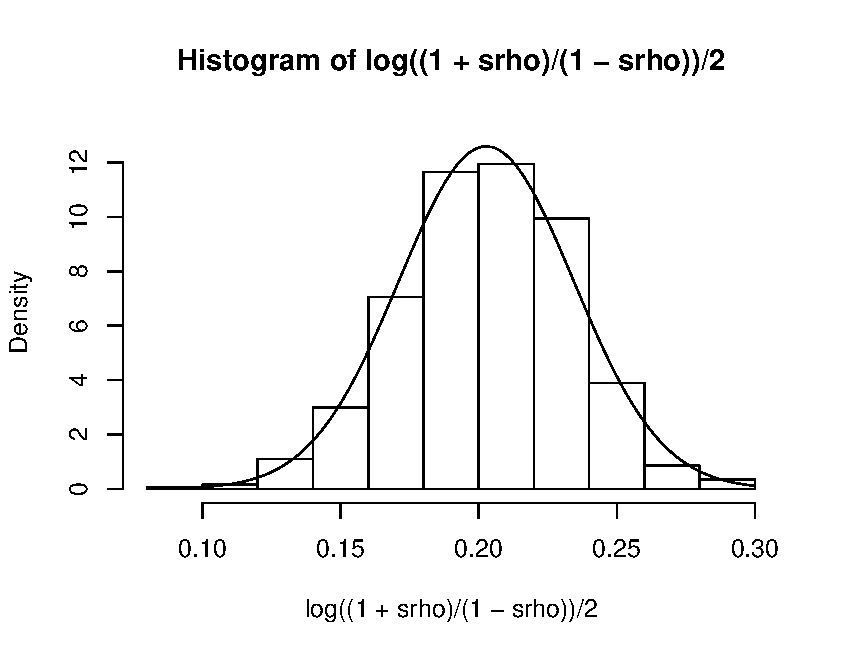
\includegraphics[scale=0.7]{pics/fisher_rho_hist}
\end{center}	
\end{frame}

\begin{frame}[fragile]{}
Fisher's z-transform test is implemented in \textsc{R} as \texttt{cor.test}.
   \begin{lstlisting}
> set.seed(1); n <- 100; rho <- 0.2
> x <- mvrnorm(n,c(0,0),matrix(c(1,rho,rho,1),2,2))
> cor.test(x[,1], x[,2], method = "pearson") 

	Pearson's product-moment correlation

data:  x[, 1] and x[, 2]
t = 6.2913, df = 998, p-value = 4.704e-10
alternative hypothesis: true correlation is not equal to 0
95 percent confidence interval:
 0.1349527 0.2542267
sample estimates:
      cor 
0.1953118 
 \end{lstlisting}
Try the same with $\rho=0$.\\[.2cm]
\begin{beamercolorbox}[wd=\paperwidth,sep=5pt]{important}
Non-gaussianity may invalidate the test and affect its power.	
\end{beamercolorbox}
\end{frame}

\begin{frame}[fragile,label=tau]{Basic nonparametric test}
\begin{alertblock}{Kendall's tau test for non-Gaussian data}
Suppose a bivariate sample $(x_i,y_i)$ for $i=1,\ldots,n$ is given.\\[.2cm]
Pair $(x_i,y_i)$ , $(x_j,y_j)$ is \alert{concordant} if $(x_i,y_i)< (x_j,y_j)$ or $(x_i,y_i)> (x_j,y_j)$. Otherwise  \alert{discordant}.\\[.2cm]
Define $\tau_{XY}\;=\;\tfrac{(\#\mbox{concordant})-(\#\mbox{discordant})}{{n\choose 2}}\;\in\;  [-1,1]$.\\[.2cm]
Test based on Kendell's $\tau$ statistic is implemented in \textsc{R} as \texttt{cor.test}.
   \begin{lstlisting}
> set.seed(1); n <- 200; rho <- 0.2; Z <- runif(n); 
> X <- runif(n)^2+sqrt(rho)*Z; Y <- runif(n)+sqrt(rho)*Z
> cor.test(X, Y, method = "pearson")$p.value
[1] 0.03417231
> cor.test(X, Y, method = "kendall")$p.value
[1] 0.01100592
 \end{lstlisting}
\end{alertblock}
\end{frame}


\begin{frame}[fragile]{Non-Gaussianity issue}
\begin{beamercolorbox}[wd=\paperwidth,sep=5pt]{important}
Vanishing covariance does not imply independence!
\end{beamercolorbox}
\begin{lstlisting}
# generate sample from two uncorrelated but dependent random variables
> set.seed(1); n <- 200
> A <- runif(n)-1/2; B <- runif(n)-1/2
> X <- t(c(cos(pi/4),-sin(pi/4)) %*% rbind(A,B))
> Y <- t(c(sin(pi/4),cos(pi/4)) %*% rbind(A,B))
> cor.test(X,Y, method = "pearson")

	Pearson's product-moment correlation

data:  X and Y
t = -0.84711, df = 198, p-value = 0.398
alternative hypothesis: true correlation is not equal to 0
95 percent confidence interval:
 -0.1971897  0.0793095
sample estimates:
        cor 
-0.06009275 \end{lstlisting}
$X$ and $Y$ are uncorrelated but dependent!
\end{frame}

\begin{frame}{}
\begin{center}
	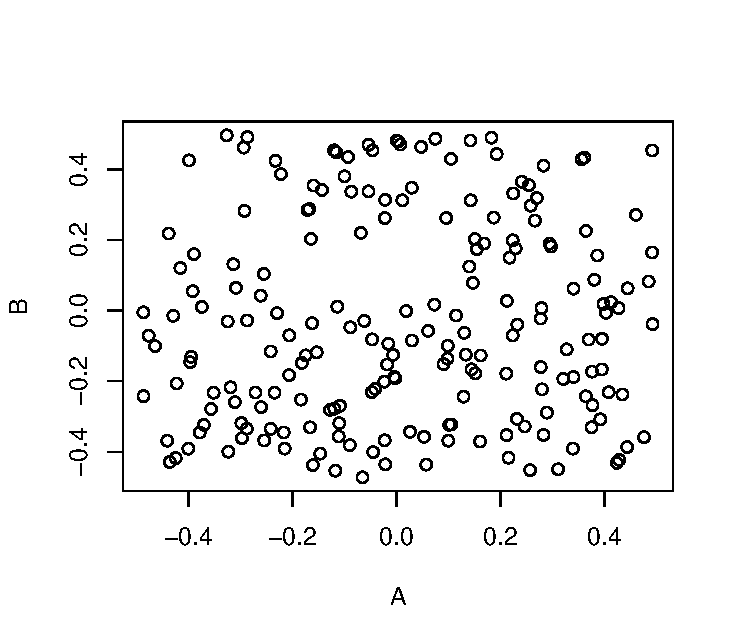
\includegraphics[width=0.5\textwidth]{pics/ABplot}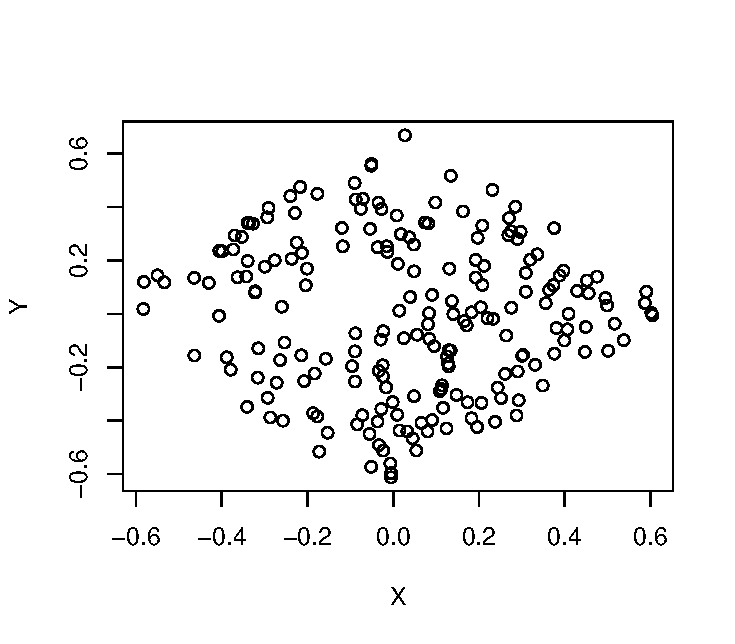
\includegraphics[width=0.5\textwidth]{pics/XYplot}	
\end{center}
	We see that $X$ and $Y$ are highly dependent. 
\end{frame}

\begin{frame}[fragile,label=zerocor]{Test based on distance correlation}
\alert{Distance correlation} $\mathcal R(X,Y)$ provides a test which applies when 
$X$, $Y$ are two random \textbf{vectors} of any dimensions.\\[.2cm]
$\mathcal R(X,Y)=0$ if and only if $X$ and $Y$ are independent.\\[.2cm]
The sample version of $\mathcal R(X,Y)$ gives a \alert{nonparametric} test of independence. \\[.2cm]
This is also implemented in R in package \texttt{energy}.
\begin{lstlisting}
> library(energy); set.seed(1); n <- 200
> A <- runif(n)-1/2; B <- runif(n)-1/2
> X <- t(c(cos(pi/4),-sin(pi/4)) %*% rbind(A,B))
> Y <- t(c(sin(pi/4),cos(pi/4)) %*% rbind(A,B))
> dcor.test(X,Y,R=1000)

	dCor independence test (permutation test)

data:  index 1, replicates 1000
dCor = 0.21161, p-value = 0.004995
sample estimates:
      dCov       dCor    dVar(X)    dVar(Y) 
0.03999654 0.21160982 0.17870935 0.19990601 
\end{lstlisting}
Here $R=1000$ is the number of the permutation bootstrap replications.
\end{frame}

\begin{frame}[fragile]{Another cautionary example}
	Bowman\& Azzalini (1997) analyse aircraft wing span and speed data.	 \begin{center}
	 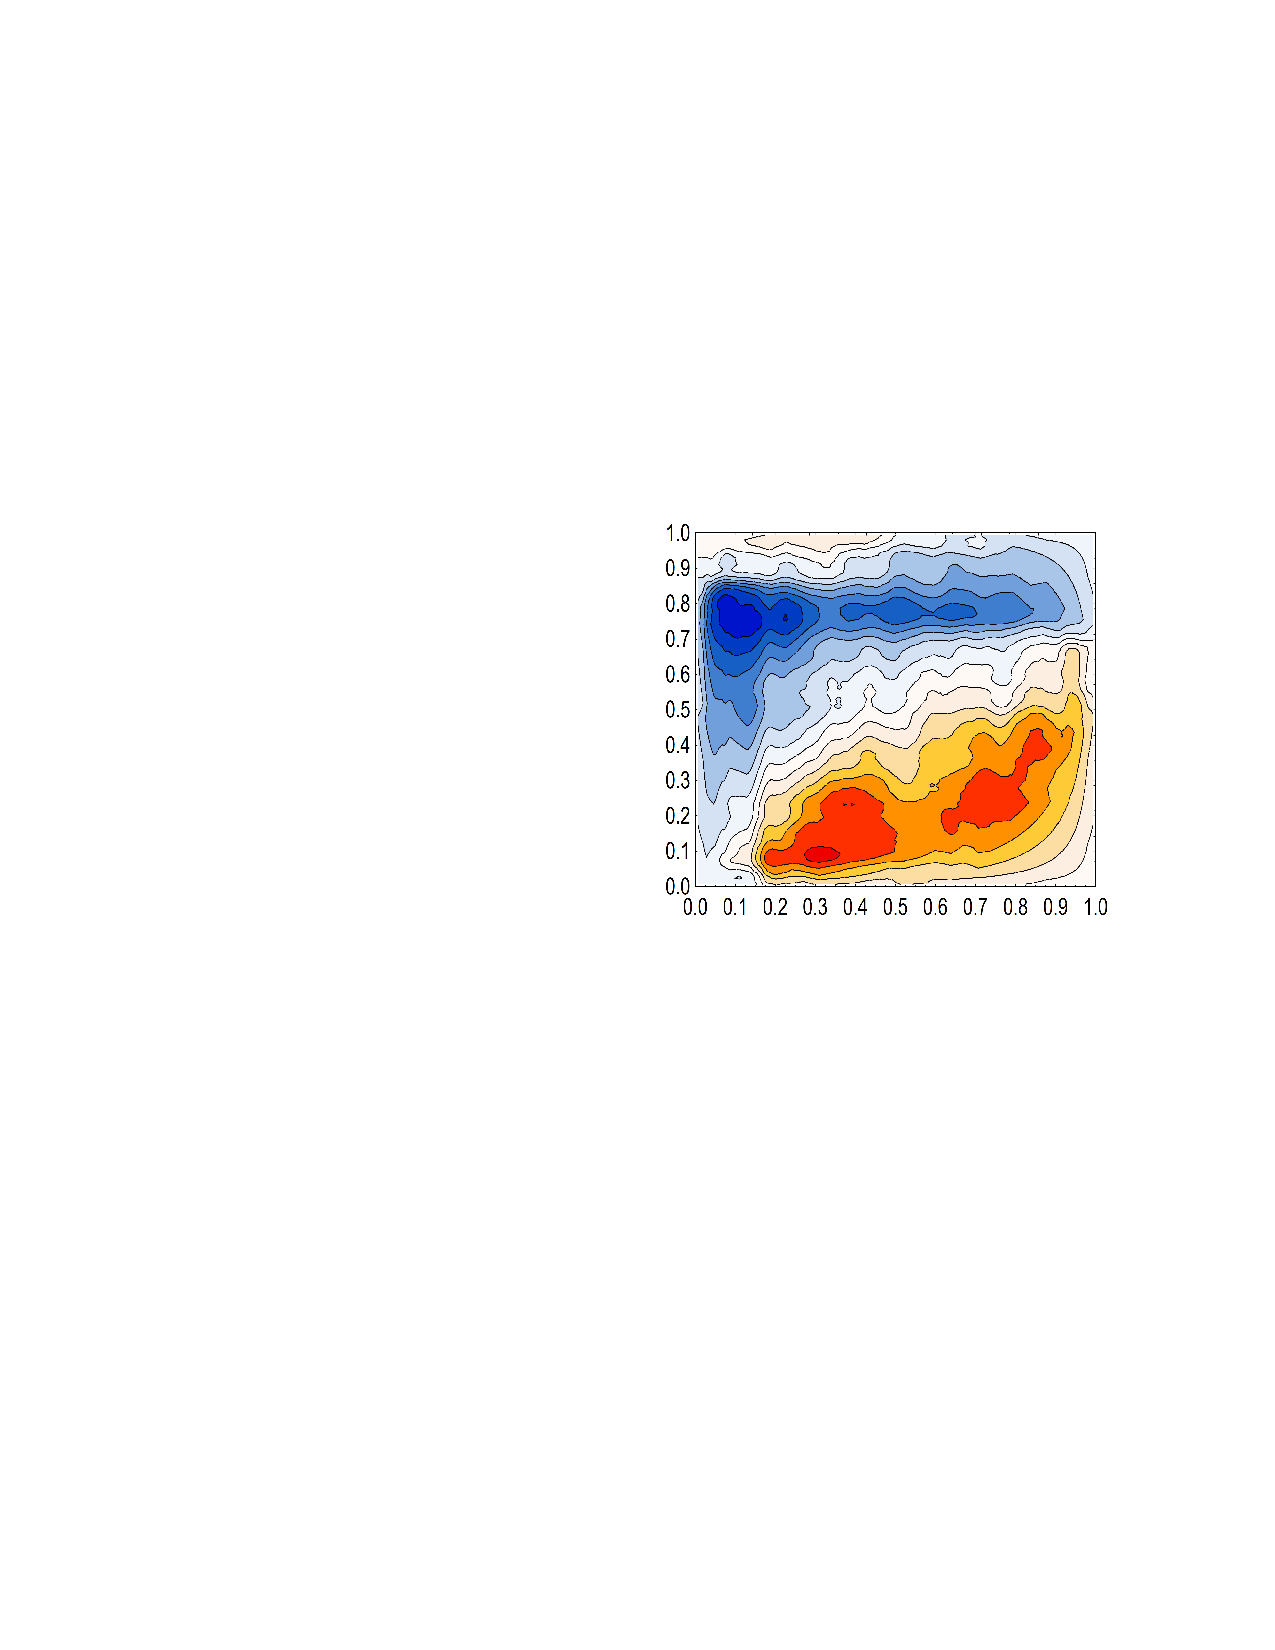
\includegraphics[scale=.6]{pics/aircraft}	 	
	 \end{center}
	 \begin{lstlisting}
> library(sm); set.seed(1); 
> X <- aircraft$Span
> Y <- aircraft$Speed
> cor.test(X,Y)$p.value
[1] 0.7816014
> dcor.test(X,Y,R=1000)$p.value
[1] 0.000999001
\end{lstlisting}

	 {\small For a discussion see: \'{C}miel, Ledwina, \textit{Validation of Association}, 2019. }
\end{frame}

\begin{frame}[fragile]{Tests for discrete data}
	\begin{alertblock}{$\chi^2$-test for discrete data}
   \begin{lstlisting}
> M <- as.table(rbind(c(762, 327, 468), c(484, 239, 477)))
> dimnames(M) <- list(gender = c("F", "M"),
+                     party = c("Democrat","Independent", "Republican"))

> (Xsq <- chisq.test(M))  # Prints test summary

	Pearsons Chi-squared test

data:  M
X-squared = 30.07, df = 2, p-value = 2.954e-07
     
> Xsq$expected   # expected counts under the null
      party
gender Democrat Independent Republican
     F 703.6714    319.6453   533.6834
     M 542.3286    246.3547   411.3166
      \end{lstlisting}
\end{alertblock}
\texttt{df = 2} is the difference between $5$ (saturated model) and $3$ (independence)
\end{frame}



\begin{frame}[fragile]{Testing conditional independence}
Testing conditional independence is hard in general.\\[.2cm] For discrete data we have an asymptotic $\chi^2$-test.\\[.2cm]

Some parametric tests are implemented in the library \texttt{bnlearn}.\\
Many non-parametric methods have been implemented in \texttt{CondIndTest}
 \begin{lstlisting}
> library(CondIndTests); library(bnlearn); set.seed(1); n <- 100
> Z <- rnorm(n); X <- 4 + 2 * Z + rnorm(n); Y <- 3 * X^2 + Z + rnorm(n)
> CondIndTest(X,Y,Z, method = "KCI")$pvalue 
[1] 2.419926e-10
> bnlearn::ci.test(X,Y,Z)$p.value 
[1] 1.15458e-25
\end{lstlisting}
\medskip

{\scriptsize See Section 3 in: 
C. Heinze-Deml, J. Peters, N. Meinshausen, Invariant Causal Prediction for Nonlinear Models, Journal of Causal Inference, 2018.}
\bigskip

{\scriptsize See: \url{http://www.bnlearn.com/documentation/man/conditional.independence.tests.html}}
\end{frame}

\begin{frame}[label=SP]{Simpson's paradox: UC Berkeley admissions example}
		The admission figures of the grad school at UC Berkeley in 1973: 8442 (44\%) men, 4321 (35\%) women admitted.\\[.3cm] The same data conditioned on the department are:\\[.3cm]
\hspace{.7cm}\begin{tabular}{|c|c|c|c|c|}
\hline
\multirow{2}{*}{Department} & \multicolumn{2}{c|}{Men}   & \multicolumn{2}{c|}{Women} \\ \cline{2-5} 
                            & Applicants & Admitted       & Applicants & Admitted       \\ \hline
A                           & 825        & 62\%          & 108        & \textbf{82\%} \\ \hline
B                           & 560        & 63\%          & 25         & \textbf{68\%} \\ \hline
C                           & 325        & \textbf{37\%} & 593        & 34\%          \\ \hline
D                           & 417        & 33\%          & 375        & \textbf{35\%} \\ \hline
E                           & 191        & \textbf{28\%} & 393        & 24\%          \\ \hline
F                           & 373        & 6\%           & 341        & \textbf{7\%}  \\ \hline
\end{tabular}
\medskip

``Measuring bias is harder than is usually assumed, and the evidence is sometimes contrary to expectation.''\\[.3cm] \tiny(Bickel et al,  \textit{Sex Bias in Graduate Admissions: Data From Berkeley}, Science, 1975) 
\end{frame}

\begin{frame}[fragile]{}
	In R:
	\begin{lstlisting}
> library(gRim); data(UCBAdmissions)
> bnlearn::ci.test(x = "Gender" , y = "Admit", z = "Dept", test="x2",data = as.data.frame(UCBAdmissions))

	Pearson's X^2

data:  Gender ~ Admit | Dept
x2 = 0, df = 6, p-value = 1
alternative hypothesis: true value is greater than 0

# gRim gives a slightly more refined output
> gRim::ciTest(as.data.frame(UCBAdmissions),set=~Gender+Admit+Dept)

set: [1] "Gender" "Admit"  "Dept"  
Testing Gender _|_ Admit | Dept 
Statistic (DEV):    0.000 df: 6 p-value: 1.0000 method: CHISQ

Slice information:
  statistic p.value df Dept
1         0       1  1    A
2         0       1  1    B
3         0       1  1    C
4         0       1  1    D
5         0       1  1    E
6         0       1  1    F
 \end{lstlisting}
% 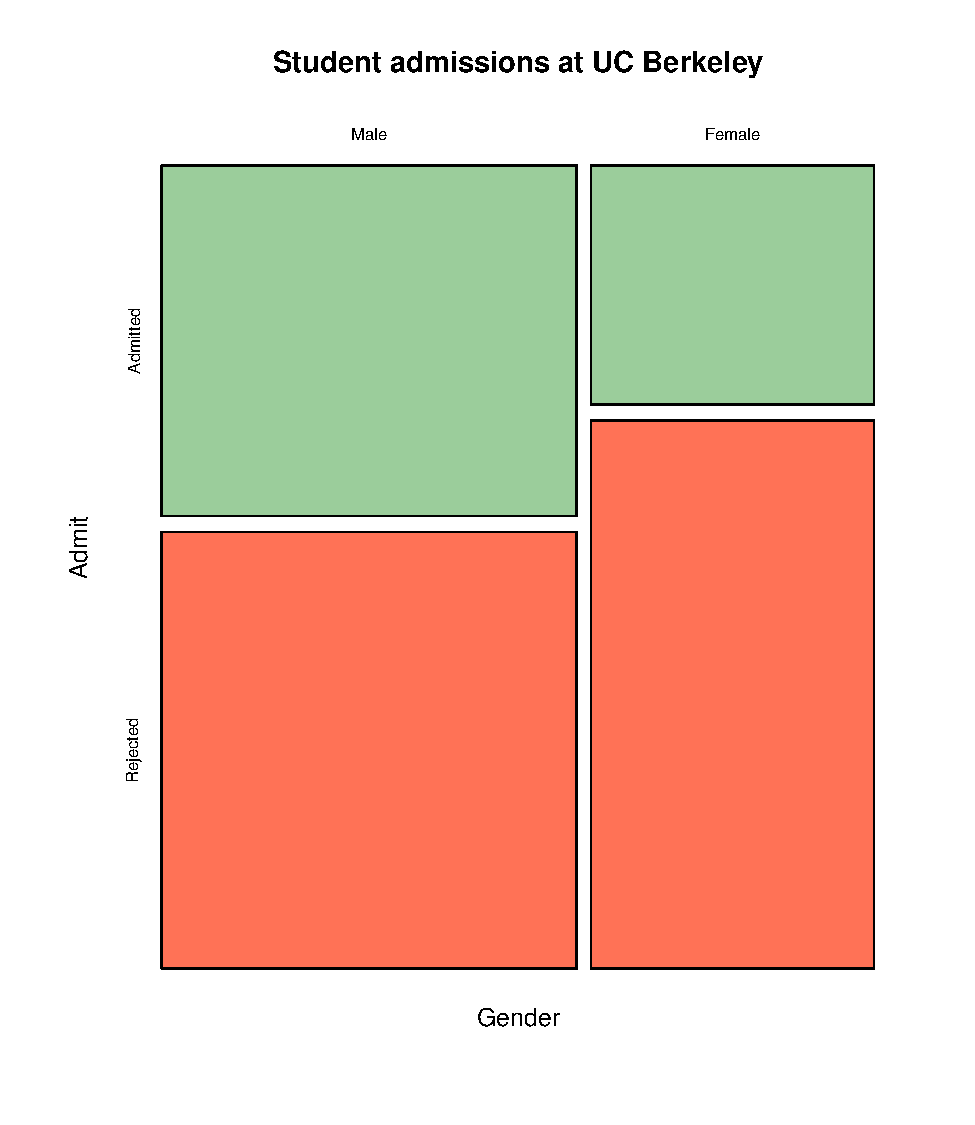
\includegraphics[scale=.3]{pics/UCB1} 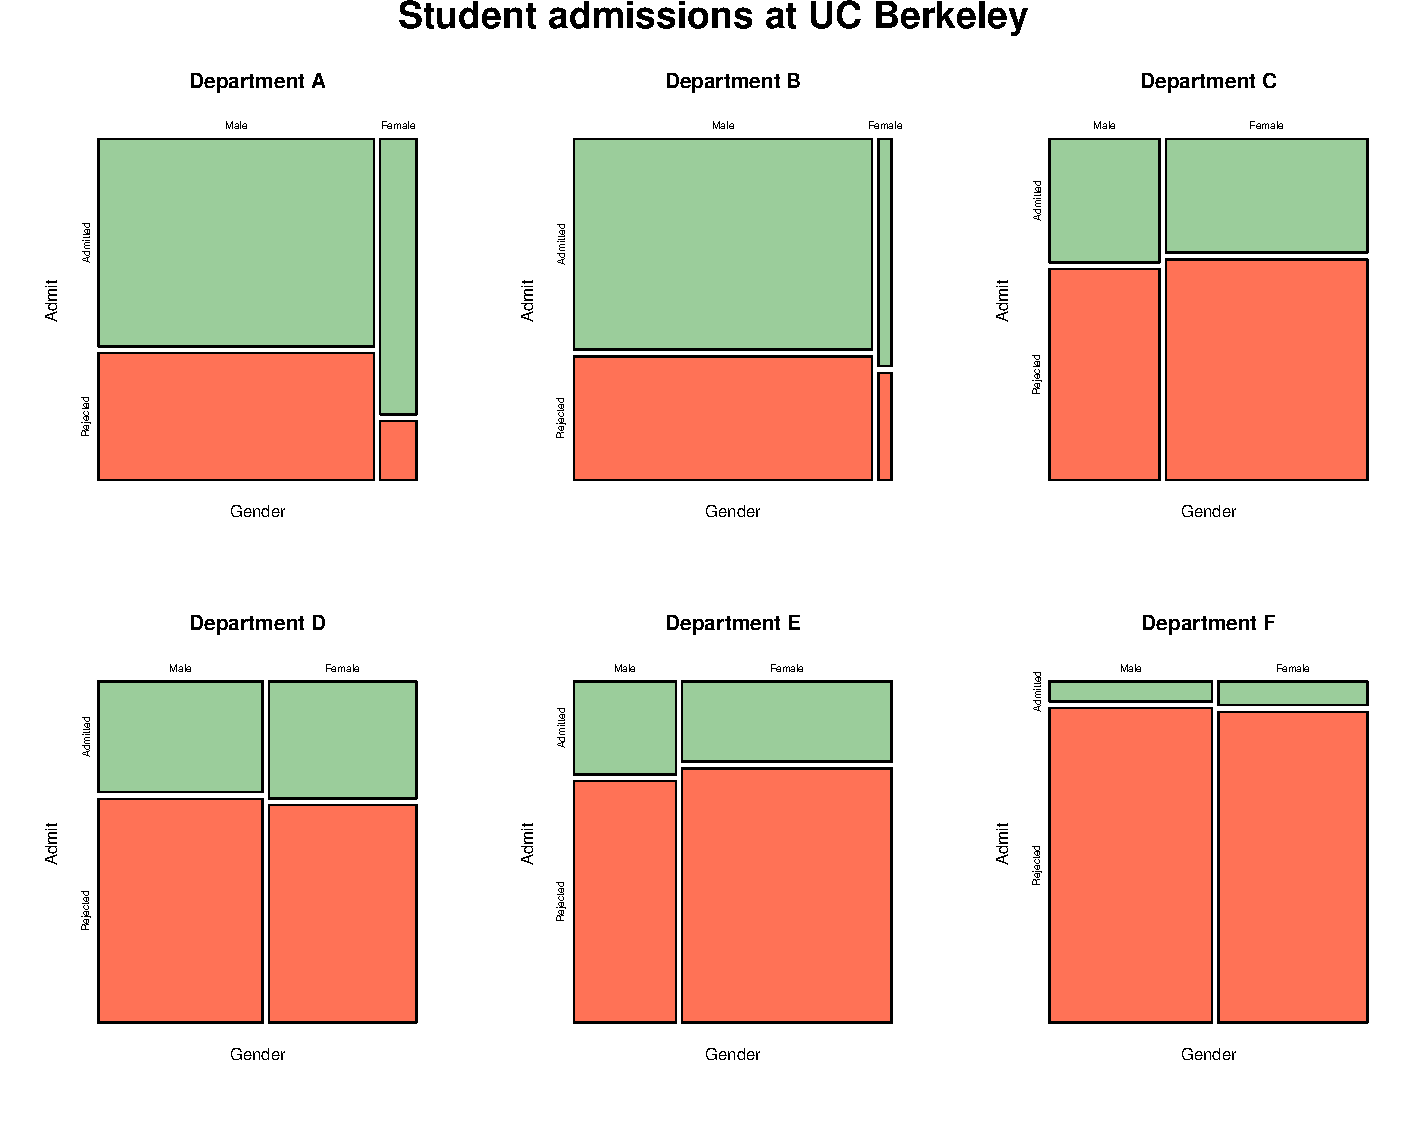
\includegraphics[scale=.3]{pics/UCB2}
\end{frame}




\begin{frame}[fragile,label=SP2]{Florida murderers}
Sentences in 4863 murder cases in Florida over the six
years 1973-78
\begin{center}
\begin{tabular}{lcc} \hline
&\multicolumn{2}{c}{Sentence}\\
\cline{2-3}
Murderer&Death&Other\\
\hline Black&59&2547\\ White&72&2185\\
\hline
\end{tabular}
\end{center}
The table shows a greater proportion
 of white murderers receiving death sentence than black
(3.2\% vs.\ 2.3\%).
	\begin{lstlisting}
> flor <- matrix(c(59,72,2547,2185),2,2)
> dimnames(flor) <- list(Murderer=c("Black","White"),Sentence=c("Death","Other"))
> chisq.test(flor)

	Pearson's Chi-squared test with Yates' continuity correction

data:  flor
X-squared = 3.6117, df = 1, p-value = 0.05737
# in the alternative we observe whites to be more often sentenced to death
\end{lstlisting}
\end{frame}

\begin{frame}[fragile]{Controlling for colour of victim}
\begin{center}
\begin{tabular}{llcc}
\hline
&&\multicolumn{2}{c}{Sentence}\\
\cline{3-4}
Victim&Murderer&Death&Other\\
\hline
Black&Black&11&2309\\
&White&0&111\\
White&Black&48&238\\
&White&72&2074\\
\hline
\end{tabular}
\end{center}
Now the table for given colour
of victim shows a very different picture.


%\pause
\smallskip

 In particular,
note that 111 white murderers killed black victims and
none were sentenced to death.
	\begin{lstlisting}
> flor <- c(11,48,0,72,2309,238,111,2074); dim(flor) <- c(2,2,2)
> dimnames(flor) <- list(Victim=c("Black","White"),Murderer=c("Black","White"),Sentence=c("Death","Other"))
> ciTest_table(flor,set=~Sentence+Murderer+Victim)
Testing Sentence _|_ Murderer | Victim 
Statistic (DEV):   67.980 df: 2 p-value: 0.0000 method: CHISQ
 \end{lstlisting}
\end{frame}


\subsection{Multivariate normal distribution}
\begin{frame}[plain,noframenumbering]{}
\begin{center}
	{\huge \textcolor{DarkRed}{1.3 Multivariate normal distribution}}
\end{center}
\end{frame}

\begin{frame}[fragile]{Recall: The density function}
%	\begin{alertblock}{Standard normal distribution}
%		Let $Z_1,\ldots,Z_p$ \textit{iid} $N(0,1)$. Their joint distribution is 
%		$$
%		f(z_1,\ldots,z_p)=\prod_{i=1}^p \left(\tfrac{1}{\sqrt{2\pi}}\exp(-\tfrac{1}{2}z_i^2)\right)=\tfrac{1}{(2\pi)^{p/2}}\exp(-\tfrac{1}{2}\bs z^T \bs z).
%		$$
%		We write $ Z=(Z_1,\ldots,Z_p)\sim N_p(\bs 0_p, \mathbb I_p)$.
%	\end{alertblock}
\begin{alertblock}{Multivariate normal distribution, $X=(X_1,\ldots,X_m)$}
Let $\mu\in \R^m$ and $\Sigma$ symmetric positive definite $m\times m$ matrix. We write $X\sim N_m(\mu,\Sigma)$ if the density of the vector $X$ is
$$
f(\bs x)=\tfrac{1}{(2\pi)^{m/2}}(\det \Sigma)^{-1/2}\exp\left(-\tfrac{1}{2}(\bs x-\mu)^T \Sigma^{-1}(\bs x-\mu)\right).
$$
\end{alertblock}

If $Z\sim N_m(\bs 0_m,\mathbb I_p)$ and \;$X=\mu+\Sigma^{1/2}Z$\; then $X\sim N_m(\mu,\Sigma)$.\\
If $X\sim N_m(\mu,\Sigma)$ then $\Sigma^{-1/2}(X-\mu)\sim N_m(\bs 0_m, \mathbb I_m)$.\\[.2cm]
To sample from $N_m(\mu,\Sigma)$ you can use \texttt{mvrnorm()} in package \texttt{MCMCpack} or 
\begin{lstlisting}
library(expm)
m <- 3; mu <- c(0,0,0); Sigma <- matrix(c(1,1/3,1/3,1/3,1,1/3,1/3,1/3,1),3,3)
n <- 1000; Z <- matrix(rnorm(m*n),m,n)
X <- mu + sqrtm(Sigma)%*%Z # sqrtm() not sqrt()!
# run cov(t(X)) to check the result
\end{lstlisting}
\end{frame}


\begin{frame}{Recall: Marginal and conditional distributions}
	Split $X$ into two blocks $X=(X_A,X_B)$. Denote $$\mu=(\mu_A,\mu_B)\qquad\mbox{and}\qquad\Sigma=\begin{bmatrix}
		\Sigma_{AA} & \Sigma_{AB}\\
		\Sigma_{BA} & \Sigma_{BB}
	\end{bmatrix}.$$
	\begin{alertblock}{Marginal distribution}
		$X_A\sim N_{|A|}(\mu_A,\Sigma_{AA})$
	\end{alertblock}
	\begin{alertblock}{Conditional distribution}
		$X_A|X_B=x_B\sim N_{|A|}\left(\textcolor{red}{\small \mu_A+\Sigma_{AB}\Sigma_{BB}^{-1}(x_B-\mu_B)},\textcolor{blue}{\small \Sigma_{AA}-\Sigma_{AB}\Sigma_{BB}^{-1}\Sigma_{BA}}\right)$
		\begin{itemize}
			\item Note that the conditional covariance is constant.
		\end{itemize}
	\end{alertblock}
%	\bigskip
%	\textbf{Example}: Consider a bivariate normal with $\mu=(0,2)$ and $\Sigma=\begin{bmatrix}
%		1 & 0.7\\0.7 & 1
%	\end{bmatrix}$. We have  $\E[X_1|X_2]={0.7}(X_2-2)$\; and\; ${\rm var}(X_1|X_2)=1-{0.7^2}= 0.51 $.
\end{frame}


\begin{frame}{Some other properties}
	\begin{alertblock}{Linear transformations}
		If $A\in \R^{m\times p}$ for $m\leq p$ and $X\sim N_p(\mu,\Sigma)$ then $AX\sim N_m(A\mu,A\Sigma A^T)$.
	\end{alertblock}
\begin{alertblock}{Moments, $X\sim N_m(\mu,\Sigma)$, $\E X=\mu$, ${\rm var}(X)=\Sigma$}
Other moments are determined by the expectation and the covariance matrix.
\end{alertblock}
\begin{alertblock}{Independence and conditional independence}
$X_i\indep X_j$ if and only if $\Sigma_{ij}=0$.\\[.3cm]
$X_i\indep X_j|X_{C}$\;\; if and only if \;\; $\Sigma_{ij}-\Sigma_{i,C}\Sigma_{C,C}^{-1}\Sigma_{C,j}=0$\\[.3cm]
Let $R=V\setminus \{i,j\}$. The following are equivalent:
\begin{itemize}
	\item $X_i\indep X_j|X_{R}$
	\item $\Sigma_{ij}-\Sigma_{i,R}\Sigma_{R,R}^{-1}\Sigma_{R,j}=0$
	\item \textcolor{blue}{$(\Sigma^{-1})_{ij}=0$}
\end{itemize}
\end{alertblock}
{\tiny Useful: \url{https://en.wikipedia.org/wiki/Block_matrix\#Block_matrix_inversion}}
%\begin{beamercolorbox}[wd=\paperwidth,sep=2pt]{notabene}	
%Central Limit Theorem provides the biggest motivation for Gaussian distributions.\end{beamercolorbox}
\end{frame}


\begin{frame}{Modelling with Gaussian distributions}
	The $m$-dimensional Gaussian distribution has $m+{m+1\choose 2}$ free parameters, which is prohibitive in high dimensions, and not very interesting from the modelling point of view.\\[.3cm]
	\begin{alertblock}{Structured covariance}
		Toeplitz, graphical models, linear covariance/concentration models, etc.
	\end{alertblock}
\begin{alertblock}{Some further limitations}
In practice distributions with heavier tails may be more suitable in certain applications.\\[.3cm] 
	The Gaussian distribution is unimodal and very symmetric (around its mean). This is sometimes too limiting.
\end{alertblock}
\end{frame}



\subsection{Graphs}

\begin{frame}[plain,noframenumbering]{}
\begin{center}
	{\huge \textcolor{DarkRed}{1.4 Graphs}}
\end{center}
\end{frame}


\begin{frame}{Basic definitions}
Graph $G=(V,E)$ with vertices $V=\{1,\ldots,m\}$ and edges $E\subset V\times V$. \\[.3cm]
\textcolor{blue}{undirected graphs}: edges have no directions, write $ij\in E$\\
directed graphs: edges have directions, write $i\to j$\\
\textcolor{blue}{directed acyclic graphs} (DAGs): directed graphs with no directed cycles.
many many more\ldots

\begin{alertblock}{In probabilistic graphical models}
	vertices represent random variables and the graph visualises the \textcolor{SeaGreen}{dependence structure}\end{alertblock}
\begin{alertblock}{In random graph models}
	the graph itself is a random variable, e.g. social networks.
\end{alertblock}
\bigskip

The term \textbf{network models} is used whenever data are visualized by graphs.
\end{frame}

%\begin{frame}{Some graph terminology}
%neighbour\\[.2cm]
%cycle\\[.2cm]
%	induced subgraph $G_A=(A,E\cap (A\times A))$\\[.2cm]
%	tree\\[.2cm]
%	adjacency matrix\\[.2cm]
%\end{frame}
%

\begin{frame}[fragile]{Package \texttt{igraph}}
The package \texttt{gRbase} popular for working with graphical models often uses the \texttt{igraph} package to work with graphs. 
\begin{lstlisting}
library(igraph)
## a basic example
> g <- graph( edges=c(1,2, 2,3, 3,1, 4,1), n=4, directed=F ) 
> plot(g) 
\end{lstlisting}
\begin{center}
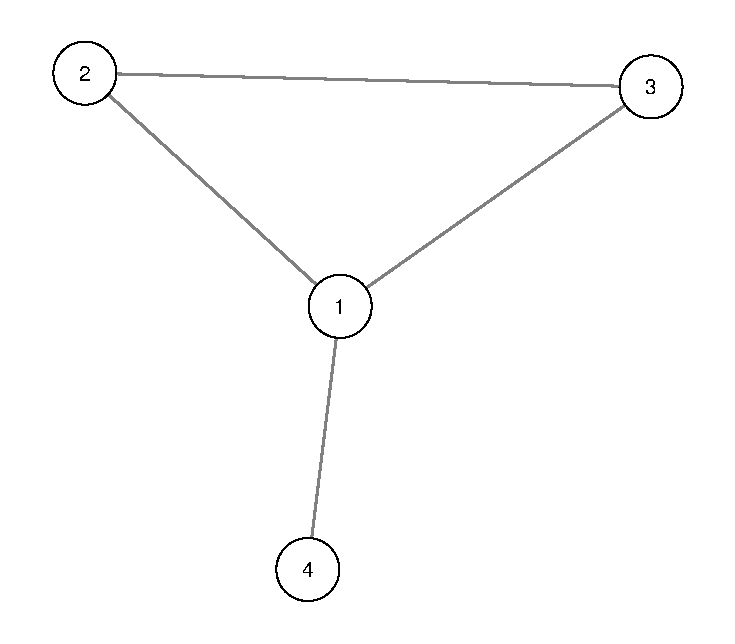
\includegraphics[scale=.5]{pics/graph1}	
\end{center}
\end{frame}

\begin{frame}[fragile]{Adjacency matrix}
The \textcolor{blue}{adjacency matrix} of a graph $G$ with $m$ nodes is an $m\times m$ matrix such that $A_{ij}=1$ if $i\to j$ in $G$ and $A_{ij}=0$ otherwise. For undirected graphs $A$ is symmetric. \\[.3cm]

The following code samples a random adjacency matrix and plots the resulting graph. 
\begin{lstlisting}
m <- 10; A <- matrix(sample(c(0,1),m^2, replace=TRUE, prob=c(0.8,0.2)),m,m);
diag(A) <- 0 # no self-loops
G <- graph_from_adjacency_matrix(A)
# plot(G)
qgraph::qgraph(A)
\end{lstlisting}
\end{frame}


\begin{frame}[fragile]{}
	\begin{lstlisting}
## an example of a tree
tr <- make_tree(40, children = 3, mode = "undirected")
plot(tr, vertex.size=10, vertex.label=NA) 
## Erdos-Renyi random graph
er <- sample_gnm(n=100, m=200) 
plot(er, vertex.size=6, vertex.label=NA)
## small-world model random graph
sw <- sample_smallworld(dim=2, size=5, nei=1, p=0.1)
plot(sw, vertex.size=6, vertex.label=NA, layout=layout_in_circle)
\end{lstlisting}
\begin{center}
	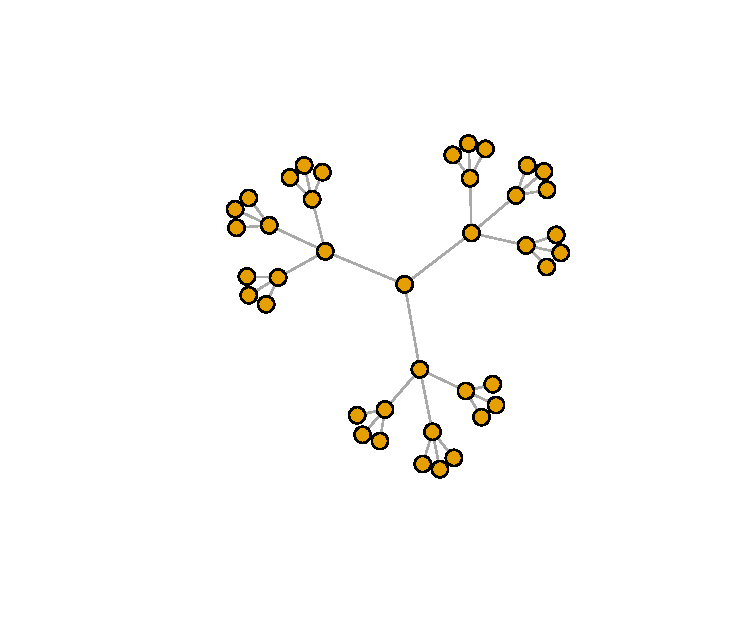
\includegraphics[width=.25\textwidth]{pics/tree1}\qquad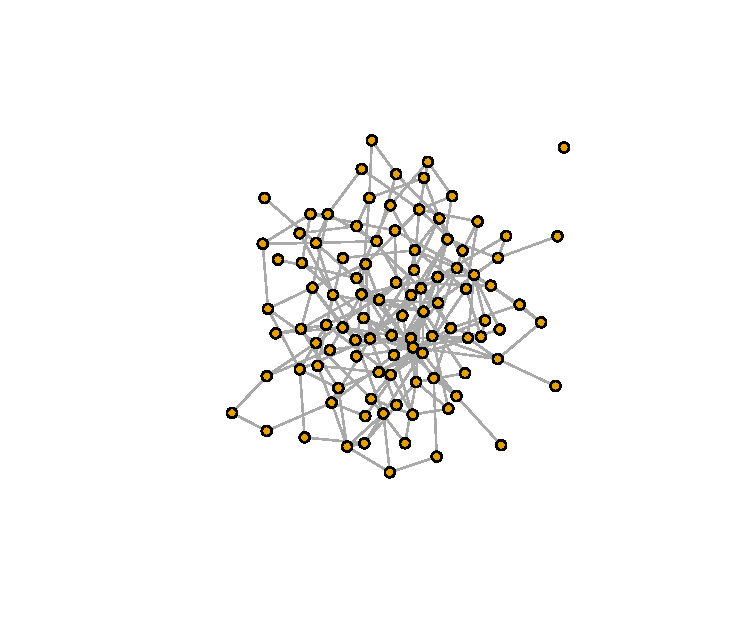
\includegraphics[width=.25\textwidth]{pics/er1}\qquad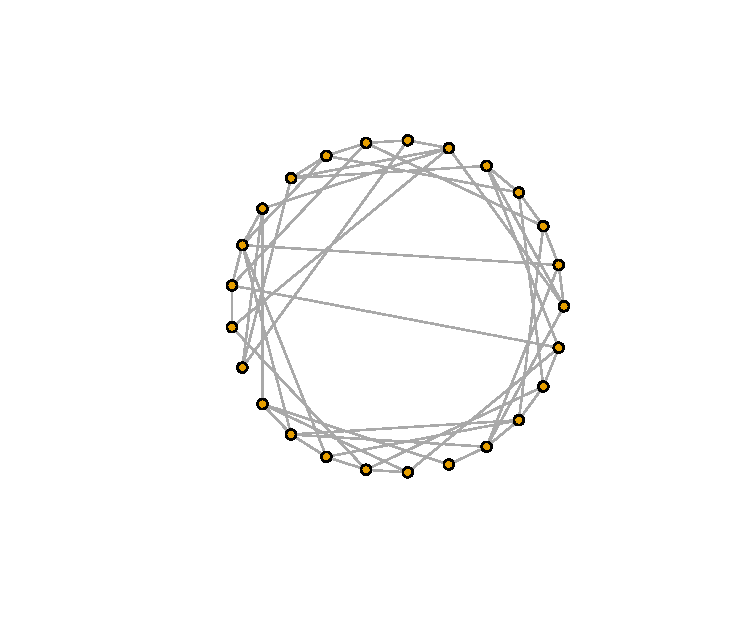
\includegraphics[width=.25\textwidth]{pics/sw1}
\end{center}
\end{frame}
%\begin{frame}[fragile]{}
%
%\begin{lstlisting}
%nodes2 <- read.csv("Dataset2-Media-User-Example-NODES.csv",header=TRUE, as.is=TRUE)
%links2 <- read.csv("Dataset2-Media-User-Example-EDGES.csv", header=TRUE, row.names=1)
%net2 <- graph_from_incidence_matrix(links2)\end{lstlisting}
%\end{frame}

\begin{frame}[fragile,label=milan]{Package \texttt{qgraph}}
Useful for simple analysis and especially in high-dimensions. 
\begin{lstlisting}
library(qgraph)
data(milan.mort,package="SemiPar")
qgraph(cor(milan.mort), layout="groups")
\end{lstlisting}
\vspace{-.3cm}
\hspace{.5cm}\begin{minipage}{5cm}
	{\tiny 
	\begin{enumerate}
		\item [day.num] number of days since 31st December, 1979
		\item [day.of.week] 1=Monday,2=Tuesday,3=Wednesday,4=Thursday, 5=Friday,6=Saturday,7=Sunday.
		\item [holiday] indicator of public holiday: 1=public holiday, 0=otherwise.
		\item [mean.temp] mean daily temperature in degrees Celcius.
		\item [rel.humid] relative humidity.
		\item [tot.mort] total number of deaths.
		\item [resp.mort] total number of respiratory deaths.
		\item [SO2]  measure of sulphur dioxide level in ambient air.
		\item [TSP] total suspended particles in ambient air.
	\end{enumerate}
	}
\end{minipage}
\begin{minipage}{6cm}
	\begin{center}
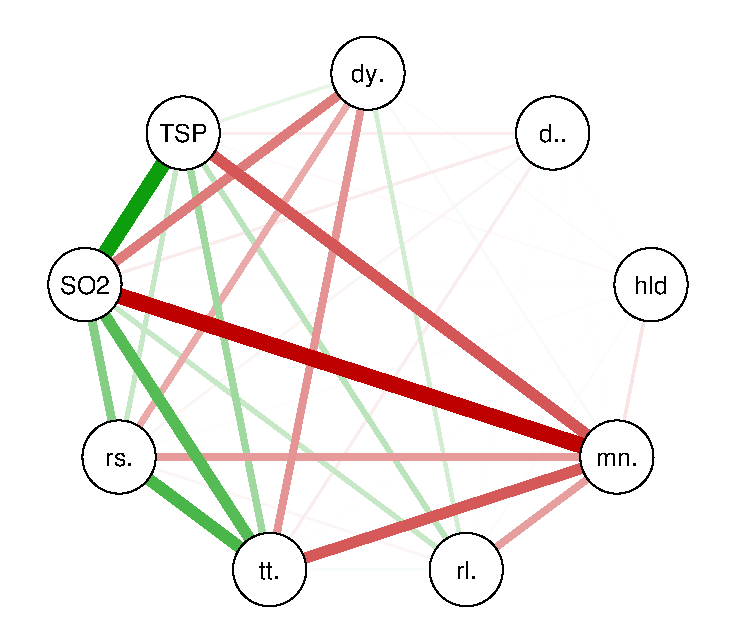
\includegraphics[scale=.5]{pics/net1}	
\end{center}
\end{minipage}

	Useful resource: \textcolor{blue}{\url{http://sachaepskamp.com/files/Cookbook.html}}
\end{frame}



\begin{frame}[fragile]{Package \texttt{gRbase}}
\texttt{gRbase} offers an interface to work with \texttt{igraph}\\[.2cm]
An \textcolor{blue}{undirected graph} can be defined by listing its \alert{maximal cliques}.
\begin{lstlisting}
> library(gRbase); library(Rgraphviz)
> ug0 <- ug(c(1,2),c(2,3,4),c(5))
> plot(ug0)
#other formats
> ug0 <- ug(c(1,2),c(2,3,4),c(5),result="igraph") #igraph
> ug0 <- ug(c(1,2),c(2,3,4),c(5),result="matrix") #adjacency matrix
> ug0
  1 2 3 4 5
1 0 1 0 0 0
2 1 0 1 1 0
3 0 1 0 1 0
4 0 1 1 0 0
5 0 0 0 0 0
> ug0 <- ug(c(1,2),c(2,3,4),c(5),result="dgCMatrix") #sparse adj. matrix
\end{lstlisting}
\begin{beamercolorbox}[wd=\paperwidth,sep=5pt]{important}
	{\small Quite conviniently \texttt{qgraph} takes as input also objects of  "graphNEL" (Rgraphviz) (and many others). This can be used to plot graphs. Run\\ \texttt{> qgraph::qgraph(ug0)}}
\end{beamercolorbox}
\end{frame}

\begin{frame}[fragile]{}
	\textcolor{blue}{Directed acyclic graph} can be given by listing sets $\{i|{\rm parents}(i)\}$
\begin{lstlisting}
> dag0 <- dag(c(1),c(2,1), c(3,1,2), c(4,3,5), c(5,1), c(7,6))
> qgraph::qgraph(dag0)
> parents("4",dag0)
[1] "3" "5"
> children("3",dag0)
[1] "4"
> ancestralSet(c("2","5"),dag0)
[1] "1" "2" "5"
#other formats, for example:
> dag0 <- dag(c(1),c(2,1), c(3,1,2), c(4,3,5), c(5,1), c(7,6), result="matrix") 
> dag0
  1 2 3 4 5 7 6
1 0 1 1 0 1 0 0
2 0 0 1 0 0 0 0
3 0 0 0 1 0 0 0
4 0 0 0 0 0 0 0
5 0 0 0 1 0 0 0
7 0 0 0 0 0 0 0
6 0 0 0 0 0 1 0\end{lstlisting}
\end{frame}

%\begin{frame}[fragile]{Converting between different formats}
%It may be 
%\begin{lstlisting}
%library(gRbase)
%library(Rgraphviz)
%ug0 <- ug(~1:2,~2:3:4,~5)
%plot(ug0)
%#other formats
%ug0 <- ug(~1:2,~2:3:4,~5,result="igraph") #igraph
%ug0 <- ug(~1:2,~2:3:4,~5,result="matrix") #adjacency matrix
%ug0 <- ug(~1:2,~2:3:4,~5,result="dgCMatrix") #sparse adj. matrix
%\end{lstlisting}
%Directed graph can be given by listing
%\end{frame}


%\subsection{Graph structure of the data}
%\begin{frame}[plain,noframenumbering]{}
%\begin{center}
%	{\huge \textcolor{DarkRed}{1.4 Graph structure of the data}}
%\end{center}
%\end{frame}
%
%\begin{frame}{General idea}
%Using graphs in data science goes far beyond data visualization.\\[.4cm]
%	Model a random vector $\bs X=(X_1,\ldots,X_d)$ looking to reduce dimensionality.\\[.4cm]
%	A possible idea is to represent dependence with a graph. 
%\end{frame}
%





\section{Undirected graphical models}

\begin{frame}[plain,noframenumbering]{}
\begin{center}
	{\Huge \textcolor{DarkRed}{Part 2: Undirected graphical models}}
\end{center}
\end{frame}


\subsection{Modelling with graphs}
\begin{frame}[plain,noframenumbering]{}
\begin{center}
	{\huge \textcolor{DarkRed}{2.1 Graph factorizations}}
\end{center}
\end{frame}

\begin{frame}{Factorization}
	$G=$ an undirected graph with nodes $\{1,\ldots,m\}$ and cliques $C_1,\ldots,C_k$.\\
	We say that density $f(\bs x)$ \textbf{\alert{factorizes according to $G$} }if for all $\bs x\in \cX$
	$$
	f(\bs x)\;=\;\phi_{C_1}(\bs x_{C_1})\cdots \phi_{C_k}(\bs x_{C_k}),
	$$ 
	where $\phi_C(\bs x_C)\geq 0$. 	(a notion of simplicity)\\[.3cm]
	
	\begin{alertblock}{For example}
		$$
	\tikzstyle{vertex}=[circle,fill=black,minimum size=5pt,inner sep=0pt]
\tikzstyle{hidden}=[circle,draw,minimum size=5pt,inner sep=0pt]
  \begin{tikzpicture}[scale=.6,baseline=5mm]
  \node[vertex] (1) at (0,2)  [label=left:$1$] {};
    \node[vertex] (2) at (2,2) [label=right:$2$]{};
    \node[vertex] (3) at (2,0) [label=right:$3$]{};
    \node[vertex] (4) at (0,0) [label=left:$4$]{};
     \draw[line width=.3mm] (2) to (1);
    \draw[line width=.3mm] (3) to (2);
    \draw[line width=.3mm] (3) to (4);
    \draw[line width=.3mm] (4) to (1);
    \draw[line width=.3mm] (1) to (3);
  \end{tikzpicture}\qquad f(\bs x)=\phi_{123}(x_1,x_2,x_3)\phi_{134}(x_1,x_3,x_4).
	$$
	\end{alertblock}
This gives an alternative characterisation of $X_2\indep X_4|(X_1,X_3)$.
\end{frame}

\begin{frame}[label=HC]{Hammersley-Clifford theorem}
Let $f>0$ be a dentity function for $\bs X=(X_1,\ldots,X_m)$. Then the following are equivalent:\\[.3cm]
\begin{enumerate}
	\item [(F)] $f$ factorizes according to $G$. \\[.4cm]
	\item [(G)] $X_A\indep X_B|X_C$ whenever $C$ \alert{separates} $A$ and $B$ in $G$.\\[.4cm]
	\item [(P)] $X_i\indep X_j|X_{V\setminus \{i,j\}}$ whenever $i,j$ not connected by an edge in $G$.
\end{enumerate}
\bigskip

The graph represents conditional independence.\\[.5cm]

\end{frame}


\begin{frame}{Graphical model $\cM(G)$}
	$G$ a graph with $m$ nodes representing a random vector $X=(X_1,\ldots,X_m)$.\\[.3cm]
	$\cM(G)$ is the family of all distributions of $X$ that factorize according to $G$. \\[.3cm]
	By the Hammersley-Clifford theorem this can be equivalently described by conditional independences. (we work with positive distributions only)
	\bigskip
	
	Model families that admit suitable factorizations are described in later parts:
\begin{enumerate}
	\item \textcolor{SeaGreen!80!black}{log-linear models} for multivariate discrete data
	\item graphical \textcolor{SeaGreen!80!black}{Gaussian models} for multivariate Gaussian data.
\end{enumerate}
This drives modelling for more complicated (non-parametric) settings.
\end{frame}

\begin{frame}{Graph analysis}
In high-dimensional scenarios we often want to learn the underlying graph from the data.\\[.3cm]
	Although graphs directly visualize the structure this still may be hard to see. \\[.3cm]
	We could be interested in:
	\begin{itemize}
		\item central vertices
		\item clusters in the network (communities)
		\item degree distribution
	\end{itemize}
	\bigskip
	Using \alert{\texttt{igraph}} seems a default option.\\[.3cm]
	A useful resource: \textcolor{blue}{\url{https://kateto.net/networks-r-igraph}}
\end{frame}

\begin{frame}[fragile]{Example of a graph analysis}
For network analysis copy your network to \texttt{igraph}:
\begin{lstlisting}
> library(sparseIndexTracking); library(xts)
> data(INDEX_2010)
> data <- INDEX_2010$X[,100:200]
> G <- qgraph::qgraph(cor(data),graph="glasso",sampleSize=nrow(data),layout="spring",threshold=.07) # takes a minute. we later discuss more scalable approaches.
> layout <- G$layout #will be used later
> G <- as.igraph(G)
# The proportion of present edges from all possible edges in the network.
> edge_density(G, loops=F)
[1] 0.04257426
\end{lstlisting}
\begin{beamercolorbox}[wd=\paperwidth,sep=5pt]{important}
	\texttt{qgraph} reports some issues but that's irrelevant for our analysis now
\end{beamercolorbox}
\end{frame}

\begin{frame}{}
	\begin{center}
		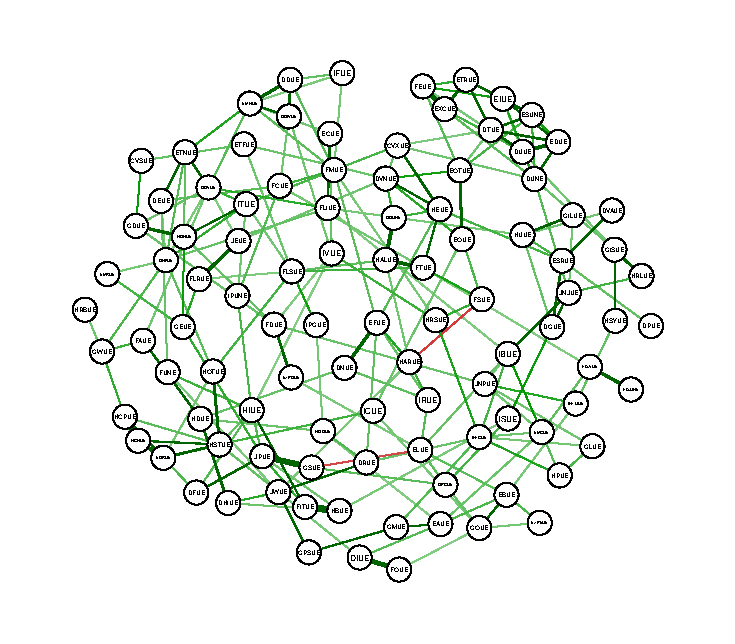
\includegraphics[scale=.9]{pics/net_analysis_ex}
	\end{center}
\end{frame}

\begin{frame}[fragile]{}
\texttt{igraph} allows for much more refined analysis
	\begin{lstlisting}
# the diameter is small!
> diameter(G, directed=F, weights=NA)
[1] 7
> deg <- degree(G, mode="all")
# check nodes with maximal degree
> which(deg==max(deg))
[1]  3  9 13 83
# plot the graph with node size and color depending on the degree
> plot(G, vertex.size=deg*2,vertex.color=deg,vertex.label=NA,layout=layout)
\end{lstlisting}
\begin{center}
	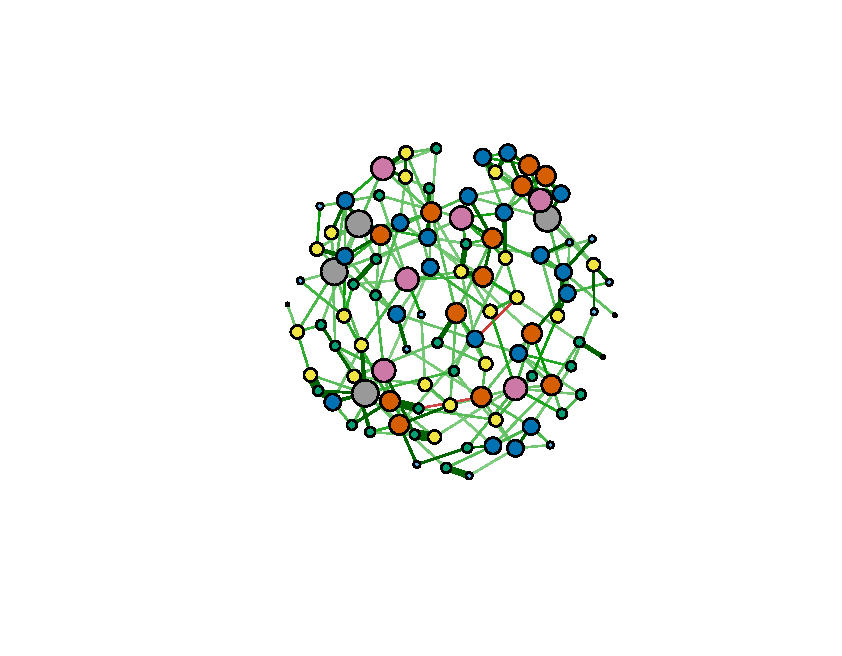
\includegraphics[scale=.7]{pics/net_analysis_ex2}
\end{center}
\end{frame}

\begin{frame}[fragile]{Centrality analysis}
	The degree is one measure of centrality of a graph.\\[.2cm]
	\alert{Closeness} is a centrality based on distance to others in the graph.
	\begin{lstlisting}
closeness(G, mode="all", weights=NA) 
E(G)$weight <- abs(E(G)$weight)
closeness(G, mode="all") 
centr_clo(G, mode="all", normalized=TRUE) 
\end{lstlisting}
Eigenvalue centrality: vertices with high eigenvector centralities are those which are connected to many other vertices which are, in turn, connected to many others (and so on). 
\begin{lstlisting}
ec <- eigen_centrality(G, directed=TRUE, weights=NA)
# there are only few vertices with high eigenvalue centrality
plot(1:length(ec$vector),ec$vector,xlab="vertex",ylab="Eigenvalue centrality")
plot(G, vertex.color=round(3*ec$vector),vertex.label.cex=.2,layout=layout)
legend(-1.2,1,legend=c("<0.33","[0.33,0.66)","[0.66,1)","1"),col=c(0,categorical_pal(3)),pch=19,cex=.4)
\end{lstlisting}
\end{frame}


\begin{frame}[plain]{}
\begin{center}
	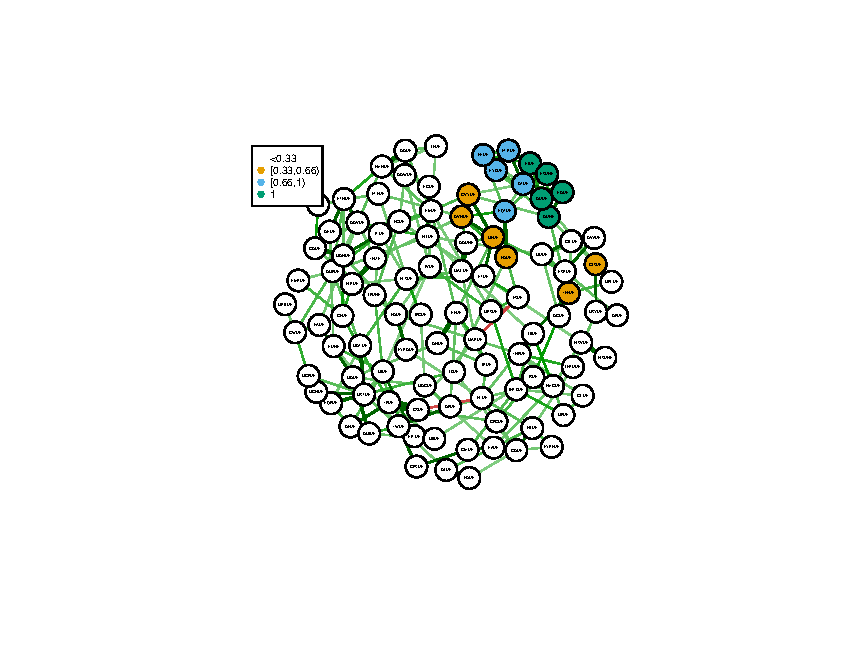
\includegraphics[scale=1.5]{pics/net_analysis_ex3}
\end{center}	
\end{frame}


\begin{frame}[fragile,plain]{Communities}
Many networks consist of modules which are densely connected themselves but sparsely connected to other modules.
\begin{lstlisting}
ceb <- cluster_edge_betweenness(G,directed=FALSE)
plot(ceb, G,vertex.label.cex=.2,layout=layout)  
\end{lstlisting}
\begin{center}
	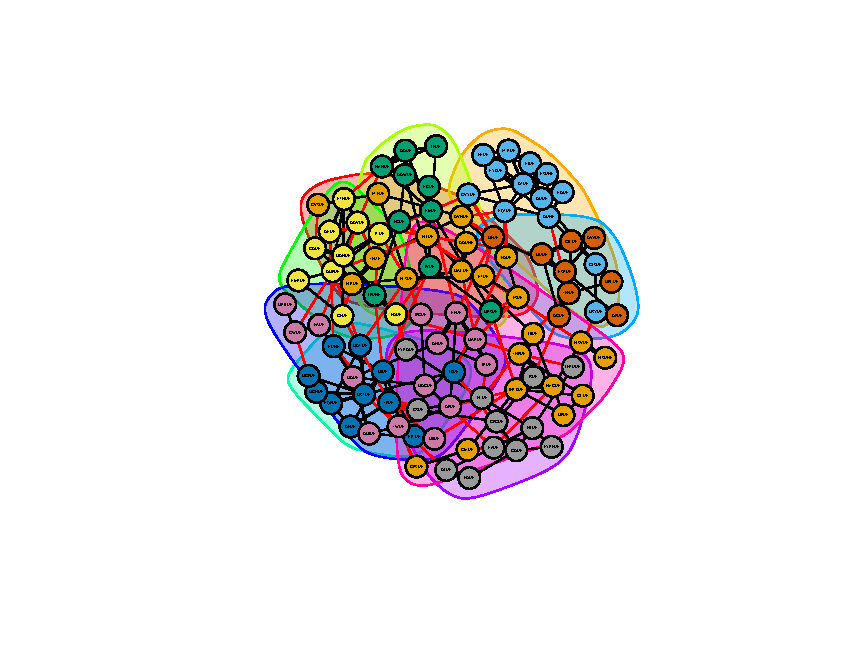
\includegraphics[scale=1]{pics/net_analysis_ex4}
\end{center}
\end{frame}

\begin{frame}[fragile]{}
\begin{lstlisting}
#coarser information possible
plot(G,vertex.color=cut_at(ceb,2),vertex.label.cex=.2,layout=layout)  \end{lstlisting}
\begin{center}
	\only<1>{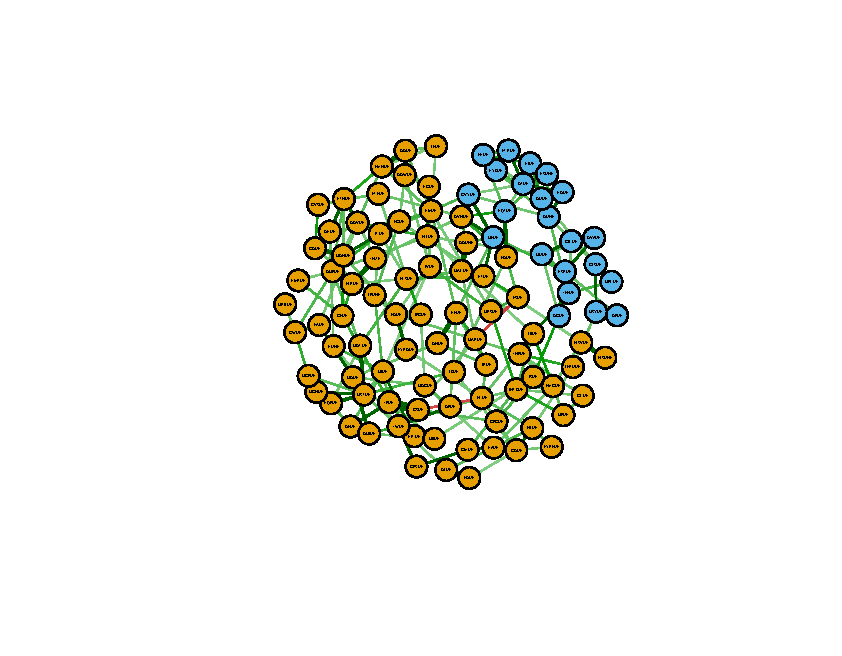
\includegraphics[scale=1.1]{pics/net_analysis_ex5a}}
	\only<2>{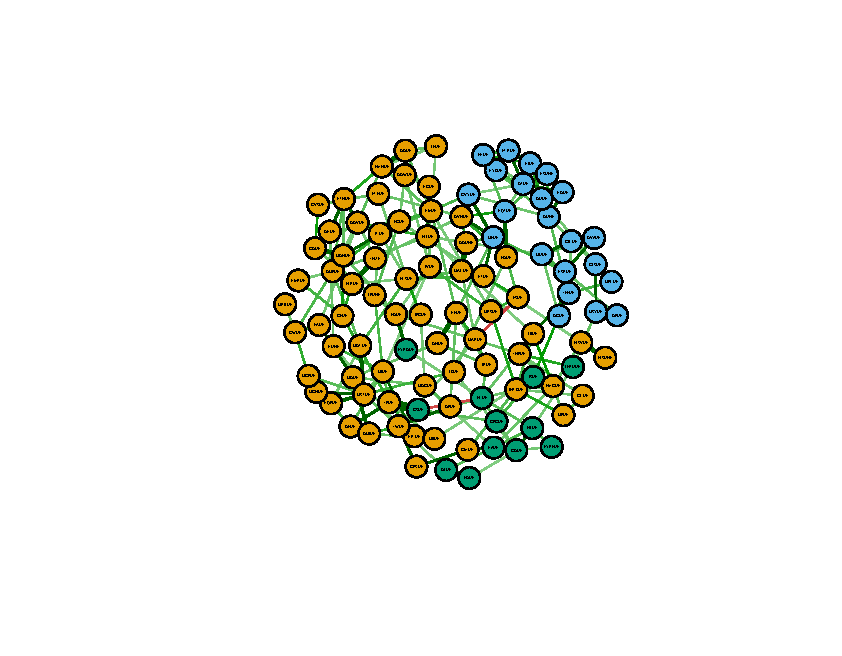
\includegraphics[scale=1.1]{pics/net_analysis_ex5b}}
	\only<3>{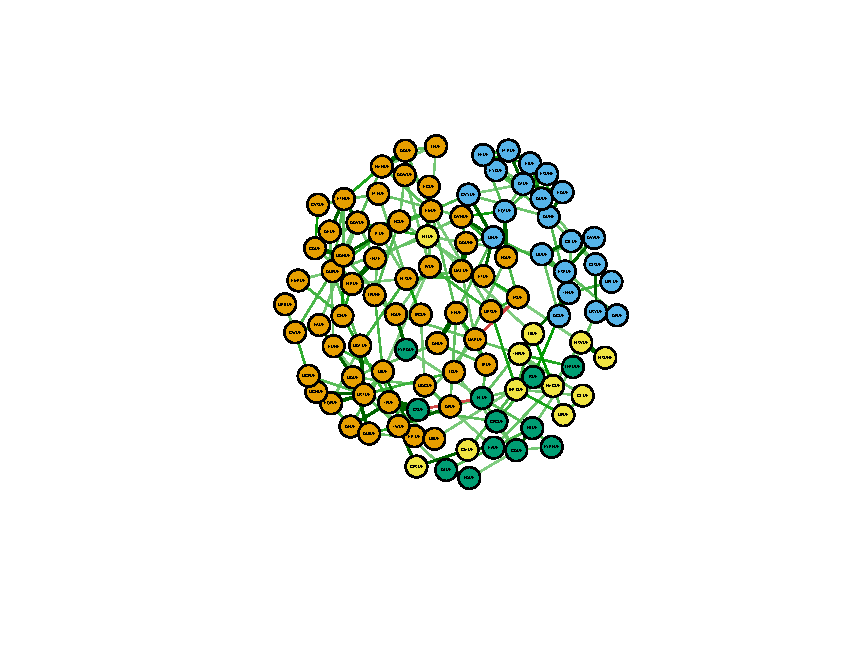
\includegraphics[scale=1.1]{pics/net_analysis_ex5c}}
\end{center}
\end{frame}



\subsection{Gaussian graphical models}
\begin{frame}[plain,noframenumbering]{}
\begin{center}
	{\huge \textcolor{DarkRed}{2.2 Gaussian graphical models}}
\end{center}
\end{frame}


\begin{frame}{The Gaussian case}
\begin{alertblock}{For a Gaussian distribution in $\cM(G)$:}
		The  non-edges of $G$ correspond to conditional independences $X_i\indep X_j|X_{V\setminus \{i,j\}}$ or equivalently \alert{$\mathbf{K_{ij}=0}$}.
		\begin{itemize}
			\item Indeed, $\rho_{ij|V\setminus \{i,j\}}=-\tfrac{K_{ij}}{\sqrt{K_{ii}K_{jj}}}$.
		\end{itemize}
\end{alertblock}
\medskip

\begin{alertblock}{Two main estimation problems:}
	Consider an \emph{iid} sample $X^{1},\ldots,X^n$ from $\cM(G)$.\\[.2cm]
The partial correlation of the sample will have no zeros.
\begin{enumerate}
	\item [(i)] Estimate $\Sigma$ for a fixed graph $G$.
	\item [(ii)] Estimate the graph in a statistically meaningful way.
\end{enumerate} 
\end{alertblock}
\end{frame}


\begin{frame}[fragile,label=samplcov]{On concentration of the covariance matrix}
%	The covariance matrix has ${m+1\choose 2}$ parameters. 
	\begin{lstlisting}
> K <- matrix(c(1,0,1/2,0,1,1/2,1/2,1/2,1),3,3); Sig <- solve(K)
> set.seed(1)
> X10 <- mvrnorm(10,c(0,0,0),Sig); S10 <- cov(X10)
> X100 <- mvrnorm(100,c(0,0,0),Sig); S100 <- cov(X100)
> X1000 <- mvrnorm(1000,c(0,0,0),Sig); S1000 <- cov(X1000)
> solve(S10); solve(S100); solve(S1000)
          [,1]     [,2]      [,3]
[1,] 1.9379597 1.616762 0.8595338
[2,] 1.6167622 4.076235 2.1360457
[3,] 0.8595338 2.136046 1.6042403
           [,1]       [,2]      [,3]
[1,] 1.04792019 0.08406772 0.5781926
[2,] 0.08406772 0.93313405 0.3880432
[3,] 0.57819258 0.38804318 1.1148584
            [,1]        [,2]      [,3]
[1,]  0.88842341 -0.02029737 0.4710935
[2,] -0.02029737  0.90492134 0.4558757
[3,]  0.47109348  0.45587568 0.9628081\end{lstlisting}
Without regularization estimating a covariance matrix is a hard problem.\\[.2cm]
Estimating the graph seems easier! (at least in this favorable case)
\end{frame}

\begin{frame}{The Gaussian likelihood function}
	The sample covariance matrix of the sample $X^{1},\ldots,X^n$ is
	$$S=\frac{1}{n}\sum_{i=1}^n(X^i-\bar X)(X^i-\bar X)^T.$$
The log-likelihood is
$$\log L(\mu,K)\;=\;\tfrac{n}{2}\log\det K-\tfrac{n}{2}\tr(KS)-\tfrac{n}{2}(\bar X-\mu)^T K(\bar X-\mu).$$
For fixed $K$ we get $\hat\mu=\bar X$ giving the \alert{profile likelihood}
$$
\log L(\hat \mu,K)\;=\;\tfrac{n}{2}\log\det K-\tfrac{n}{2}\tr(KS).
$$
\end{frame}

\begin{frame}{Maximizing the likelihood over $\mathcal M(G)$}
$\cM(G)$ consists of PD matrices $K$ such that $K_{ij}=0$ for $ij\notin E$. \\[.3cm]

	Optimizing $\log L(\hat \mu,K)$ over $\cM(G)$ is a convex optimization problem.\\[.3cm]
	The MLE is the \textcolor{SeaGreen}{unique} point $\hat\Sigma$ such that:
	\begin{enumerate}
		\item [(i)] $\hat\Sigma_{CC}=S_{CC}$ for all cliques $C$,
		\item [(ii)] $\hat K_{ij}=0$ for all $ij\notin E$.
	\end{enumerate}
	\begin{alertblock}{Maximization}
		Typically numerically using a block \textcolor{SeaGreen}{coordinate-descent} scheme (\texttt{ggmfit}).
		%If $G$ is decomposable, the MLE admits a closed-form solution.
	\end{alertblock}
		\begin{alertblock}{The deviance}
		Gives the likelihood ratio statistic to test against the unconstrained model. 
	\end{alertblock}
\end{frame}

\begin{frame}[fragile]{}
	Using \texttt{gRbase}, \texttt{gRim}, \texttt{RBGL}:
\begin{lstlisting}
> data(carcass)
# generate model: use plot(gen.carc) to see the graph
> glist <- list(c("Fat11","Fat12","Meat12", "Meat13"), c("Fat11","Fat12","Fat13","LeanMeat"),c("Meat11","Meat12","Meat13"),c("Meat11","Fat13","LeanMeat"))
#cmod specifies graphical Gaussian model ('c' for continuous)
> gen.carc <- cmod(glist,data=carcass,fit=TRUE)
# the deviance is large
> gen.carc$fitinfo$dev; 1-pchisq(gen.carc$fitinfo$dev,6)
[1] 19.78537
[1] 0.003023752
> qgraph::qgraph(-cov2cor(gen.carc$fitinfo$K))
# more direct way that also gives more flexibility
> carcfit <- ggmfit(S.carc,n=nrow(carcass),glist,eps = 1e-14,iter=10000)

  \end{lstlisting}
\end{frame}

\begin{frame}{Coordinate descent}
\begin{itemize}
	\item Coordinate descent is a classic optimisation technique for multidimensional functions; the idea is to optimise with respect to one variable at a time, holding the others constant, cycling through all variables in some given order repeatedly, until convergence.
	\item Convex functions are convex in each coordinate.
	\item This gives the global minimum under some additional conditions. 
\end{itemize}
\begin{alertblock}{Old idea in statistics\ldots}	
\begin{itemize}
\item Iterative Proportional Fitting for log-linear models dates back to Bartlett (1935), Csisz\'{a}r (1970s).
	\item Gaussian graphical models: Dempster (1972), Wermuth and Scheidt (1977), Speed and Kiiveri (1982).
\end{itemize}
\end{alertblock}
\end{frame}


\begin{frame}{When coordinate descent works?}
\begin{alertblock}{Your intuition is correct}
	\begin{itemize}
		\item If $f$ is continuously differentiable and strictly convex  then coordinate descent converges to the global optimum.
	\end{itemize}
\end{alertblock}
\begin{alertblock}{Separability condition}
	\begin{itemize}
		\item Suppose $f(\beta)=g(\beta)+\sum_{j=1}^p h_j(\beta_j)$
		\begin{itemize}
		\item $g:\R^p\to \R$ differentiable and convex
		\item $h_j:\R\to\R$ are convex  
	\end{itemize}
	\item Tseng (1988,2001): in this scenario coordinate descent converges to the global optimum
	\end{itemize}
\end{alertblock}\end{frame}


%\begin{frame}{On regularized concentration}
%	Recall example on Slide~\ref{samplcov}.
%	\begin{lstlisting}
%# generate model
%> glist <- list(c("V1","V3"), c("V2","V3"))
%> gen10 <- cmod(glist,data=as.data.frame(X10))
%> fit10 <- ggmfit(cov(as.data.frame(X10)),n=10,glist)
%> fit100 <- ggmfit(cov(as.data.frame(X100)),n=100,glist)
%> fit1000 <- ggmfit(cov(as.data.frame(X1000)),n=1000,glist)
%  \end{lstlisting}
%
%\end{frame}

\begin{frame}{Model selection methods}
How to learn the graph:\\[.4cm]
\begin{itemize}
	\item Stepwise methods,\\[.4cm]
	\item  Thresholding,\\[.4cm]
	\item Convex optimization,\\[.4cm]
	\item Simultaneous $p$-values.  (not discussed here)
\end{itemize}	
\end{frame}


\begin{frame}[fragile,label=carcass_stepwise]{Stepwise methods}
%	\begin{alertblock}{Stepwise backward model selection}
	The \texttt{stepwise} function in \texttt{gRim} performs stepwise model selection based on a variety of criteria (AIC, BIC, etc)	
	\begin{lstlisting}
sat.carc <- cmod(~.^.,data=carcass); n <- nrow(carcass)
test.carc <- stepwise(sat.carc,details=1,criterion="aic",type="decomposable",k=log(n))
# plot(test.carc) or using the qgraph package
Sigma.hat <- solve(test.carc$fitinfo$K)
qgraph::qgraph(Sigma.hat,graph="pcor") 
\end{lstlisting}
%	\end{alertblock}
%	\begin{alertblock}{BIC model selection}
%		s
%	\end{alertblock}
\begin{center}
%	{\tiny\begin{table}[ht]
%\centering
%\begin{tabular}{rrrrrrrr}
%  \hline
% & F11 & M11 & F12 & M12 & F13 & M13 & LM \\ 
%  \hline
%F11 & 0.44 & 0.02 & -0.20 & -0.07 & -0.16 & 0.05 & 0.10 \\ 
%  M11 & 0.02 & 0.16 & -0.03 & -0.06 & -0.04 & -0.05 & -0.03 \\ 
%  F12 & -0.20 & -0.03 & 0.54 & 0.06 & -0.20 & -0.04 & 0.09 \\ 
%  M12 & -0.07 & -0.06 & 0.06 & 0.14 & 0.00 & -0.09 & 0.00 \\ 
%  F13 & -0.16 & -0.04 & -0.20 & 0.00 & 0.55 & 0.00 & 0.07 \\ 
%  M13 & 0.05 & -0.05 & -0.04 & -0.09 & 0.00 & 0.16 & -0.02 \\ 
%  LM & 0.10 & -0.03 & 0.09 & 0.00 & 0.07 & -0.02 & 0.27 \\ 
%   \hline
%\end{tabular}
%\end{table}}
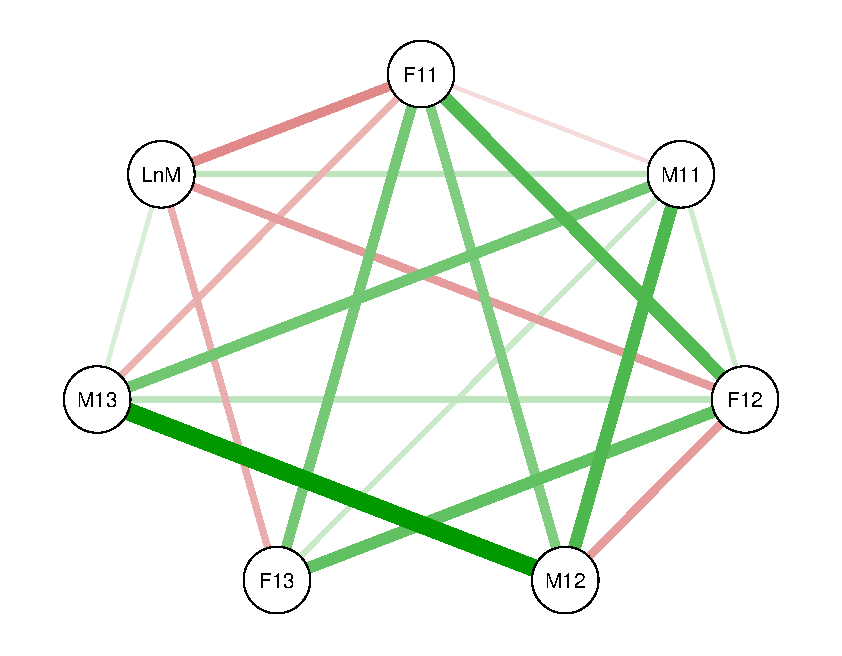
\includegraphics[scale=.45]{pics/carcass}
\end{center}
\end{frame}

\begin{frame}{Thresholding}
	A simple and natural method is to threshold entries of the sample concentration matrix. \\[.3cm]
	Some obvious issues:
	\begin{itemize}
		\item The sample covariance matrix $S$ is not invertible if $n<m$. 
		\item Thresholded $S^{-1}$ may not be positive definite. 
		\item The approach is not statistically sound.
	\end{itemize}
\end{frame}

\begin{frame}[fragile]{Thresholding}
Consider example on Slide~\ref{carcass_stepwise}
	\begin{lstlisting}
> data(carcass); S.carc <- cov(carcass); PC.carc <- cov2pcor(S.carc)
> threshold <- 0.1
# define the thresholded version of PC.carc
> PC.thresh <- PC.carc; PC.thresh[abs(PC.thresh)<threshold] <- 0
> qgraph::qgraph(PC.thresh) # visually similar to the stepwise case
# compare this with the stepwise selection graph
> cmod(PC.thresh,data=carcass)
Model: A cModel with 7 variables
 -2logL    :       11384.93 mdim :   23 aic :     11430.93 
 ideviance :        2456.30 idf  :   16 bic :     11519.27 
 deviance  :          17.48 df   :    5 
 
 >  test.carc
Model: A cModel with 7 variables
 -2logL    :       11370.74 mdim :   25 aic :     11420.74 
 ideviance :        2470.49 idf  :   18 bic :     11516.76 
 deviance  :           3.29 df   :    3 
\end{lstlisting}
\end{frame}



\begin{frame}[fragile]{Learning the graph in high-dimension}
\begin{alertblock}{Graphical lasso}
	If the dimension $m$ is large then the number of possible models is too high.\\[.2cm]


Following the same idea as in the lasso regression we maximize
$$
L_{\rm pen}(K,\hat \mu)\;=\;\log\det (K)-\tr(SK)-\alert{\lambda \|K\|_1}.
$$
See the package \texttt{glasso} and \texttt{EBICglasso} (finds an optimal $\lambda$).
\end{alertblock}
\begin{alertblock}{Example: Personality traits}
\begin{lstlisting}
> d <- read.table("./data/personality0.txt"); S <- cor(d)
# the partial correlation graph of the data is dense
> qgraph::qgraph(S,graph="pcor")
# the glasso graph is much sparser
> qgraph::qgraph(S,graph="glasso",sampleSize=nrow(d),layout="spring")
\end{lstlisting}
	The estimated graph has  137 edges compared to 496 of the full graph.
\end{alertblock}
\end{frame}

\begin{frame}[plain,label=pers_lasso]{}
	\begin{center}
		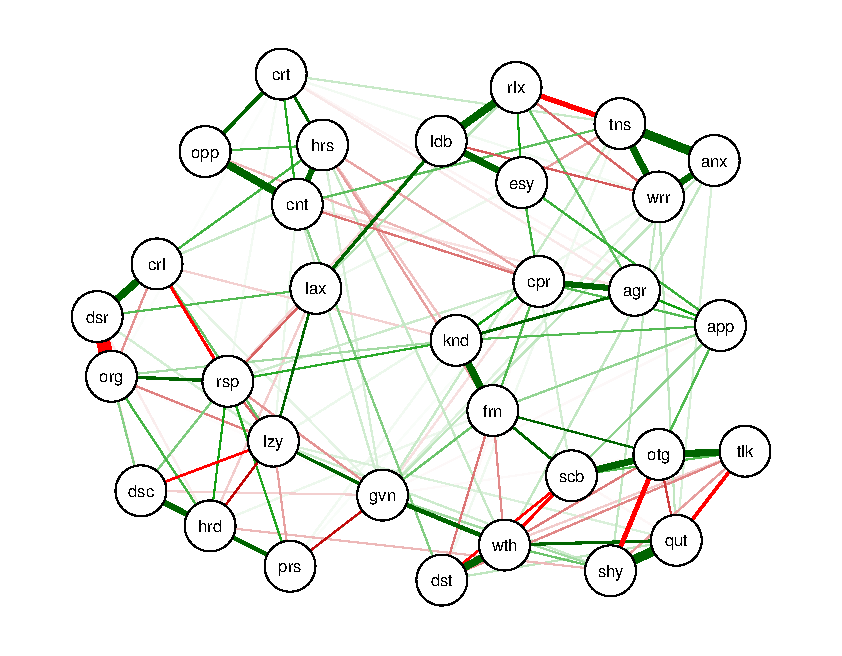
\includegraphics[scale=.9]{pics/personality_lasso}
	\end{center}
\end{frame}

\begin{frame}{EBIC graphical lasso}
	EBIC provides a data-driven way to choose the penalty parameter $\lambda$ in graphical lasso.
	
	\begin{enumerate}
		\item Run the graphical lasso for a range of penalty parameters to get a preselected list of models.\\[.2cm]
		\item For the models in the above list maximize the EBIC for $\gamma\in [0,1]$: $${\rm BIC}_\gamma\;=\;-2\ell_n(\hat K)+|E|\log n+4|E|\gamma\log p.$$
	\end{enumerate}
	Consistency of ${\rm EBIC}$ has been shown under some technical assumptions (Drton, Foygel, 2010).\\[.2cm] Simulations show that consistency holds under much weaker conditions.\\[.2cm]
	The procedure is much quicker than CV. 
\end{frame}


\begin{frame}{Main papers on graphical Lasso}
Basic asymptotic theory studied in:\\
	{\scriptsize Yuan \& Lin (2007). Model selection and estimation in the Gaussian graphical model. Biometrika, 94(1), 19-35. }\\[.3cm]

Alternative optimization methods + the name:\\	
	{\scriptsize 	Friedman, Hastie \& Tibshirani (2008). Sparse inverse covariance estimation with the graphical lasso. Biostatistics, 9(3), 432-441.}\\[.1cm]
	{\scriptsize 	d'Aspremont, Banerjee \& El Ghaoui (2008). First-order methods for sparse covariance selection. SIAM Journal on Matrix Analysis and Applications, 30(1), 56-66.}\\[.3cm]
	
	Non-asymptotic theory studied in:\\
	{\scriptsize Ravikumar, Wainwright, Raskutti \& Yu (2011). High-dimensional covariance estimation by minimizing $\ell 1$-penalized log-determinant divergence. Electronic Journal of Statistics, 5, 935-980.}\\[.2cm]
	\begin{beamercolorbox}[wd=\paperwidth,sep=5pt]{important}
Under some extra conditions we get: 	$\|\hat K-K^*\|=\mathcal O\left(\sqrt{\min\{d^2,s+m\}\tfrac{\log m}{n}}\right)$	 and model selection consistency.
	\end{beamercolorbox}
\end{frame}

\begin{frame}[fragile]{We assume sparsity!}
The sparsity or bounded degree assumption are not always justified.\\ Consider the data set from Slide~\ref{milan}.
\begin{lstlisting}
data(milan.mort,package="SemiPar")
qgraph::qgraph(cor(milan.mort), layout="groups", graph="glasso",sampleSize=nrow(milan.mort)) # outputs some warnings
# traditional model selection
sat.mort <- cmod(~.^.,data=milan.mort)
test.mort <- stepwise(sat.mort,details=1,"test")
qgraph::qgraph(-cov2cor(test.mort$fitinfo$K)) # essentially the same graph
\end{lstlisting}
\vspace{-.3cm}
\hspace{.5cm}\begin{minipage}{5.5cm}
	{\tiny 
	\begin{enumerate}
		\item [day.num] number of days since 31st December, 1979
		\item [day.of.week] 1=Monday,2=Tuesday,3=Wednesday,4=Thursday, 5=Friday,6=Saturday,7=Sunday.
		\item [holiday] indicator of public holiday: 1=public holiday, 0=otherwise.
		\item [mean.temp] mean daily temperature in degrees Celcius.
		\item [rel.humid] relative humidity.
		\item [tot.mort] total number of deaths.
		\item [resp.mort] total number of respiratory deaths.
		\item [SO2]  measure of sulphur dioxide level in ambient air.
		\item [TSP] total suspended particles in ambient air.
	\end{enumerate}
	}
\end{minipage}
\begin{minipage}{6cm}
	\begin{center}
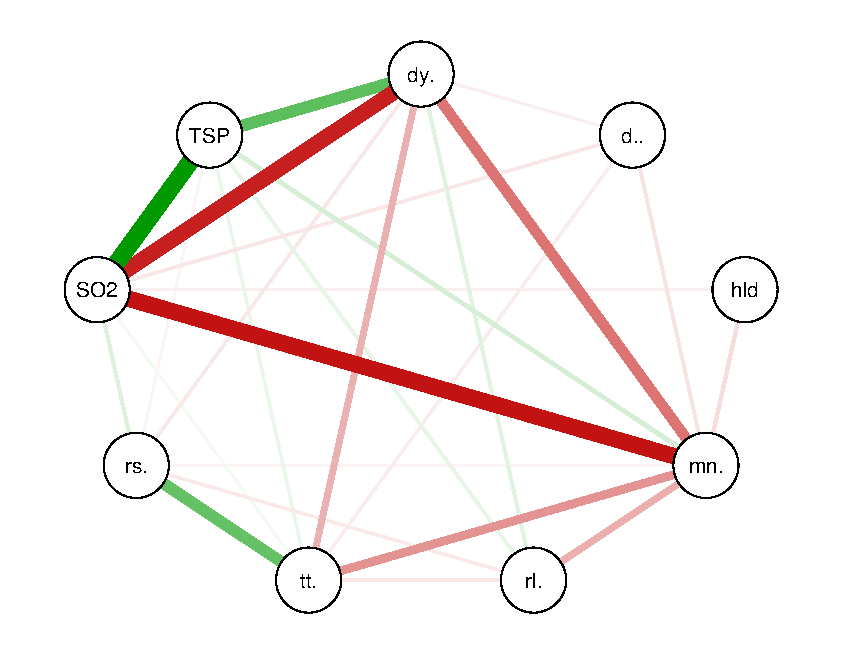
\includegraphics[scale=.4]{pics/net2}	
\end{center}
\end{minipage}	
{\small (Note on ${\rm TSP}-{\rm dy.}$ and ${\rm TSP}-{\rm mn.}$)}
\end{frame}



\begin{frame}{CLIME estimator}
Alternative to graphical lasso:\\[.4cm]
	Instead of maximizing the log-likelihood, CLIME estimator finds a sparse estimate of the precision matrix by solving
	$$
	\hat K\;=\;\arg\min \|K\|_1\quad\mbox{subject to } \|SK-\mathbb I_p\|_\infty \leq \lambda.
	$$
	\begin{itemize}
		\item similar consistency guarantees as graphical lasso,
		\item computationally attractive,
		\item implemented in the $\texttt{R}$ package \texttt{clime}.
	\end{itemize}
\end{frame}



\subsection{Log-linear models}

\begin{frame}[plain,noframenumbering]{}
\begin{center}
	{\huge \textcolor{DarkRed}{2.3 Log-linear models}}
\end{center}
\end{frame}


\begin{frame}{Hierarchical models}
	State space $\cX=\cX_1\times \cdots\times \cX_m$,\quad  $|\cX_i|<+\infty$.\\[.2cm]
	Simplicial complex: $\cC_0$ set of subsets of $\{1,\ldots,m\}$ such that
	\begin{itemize}
	\item $\{i\}\in \cC_0$ for all $i=1,\ldots,m$,
	\item $C\in \cC_0$ and $A\subset C$ then $A\in \cC_0$
\end{itemize}

	\alert{Generators}: Denote by $\cC$ the maximal elements of $\cC_0$.\\[.4cm]
	

	\begin{beamercolorbox}[wd=\paperwidth,sep=3pt]{important}
		\textbf{The model}: $p(x)\;=\;\prod_{C\in \cC} \phi_C(x_C)$, \;\;where $\phi_C>0$.
	\end{beamercolorbox}
	\bigskip
	
	\textcolor{SeaGreen}{Main effect model}: $\cC=\{\{1\},\ldots,\{m\}\}$.\\[.3cm]
	\textcolor{SeaGreen}{Pairwise interaction model}: $\cC=\{\mbox{all pairs}\}$.\\
	\qquad $\bullet$ more generally: edges of a graph with m nodes.
\end{frame}

\begin{frame}{Graphical and non-graphical models}
	(Graphical) hierarchical models: $\cC$ be the set of maximal cliques of $G$.\\[.3cm]
	Hammersley-Clifford theorem (Slide~\ref{HC}) gives equivalent description in terms of conditional independences.\\[.3cm]
	
		\begin{beamercolorbox}[wd=\paperwidth,sep=3pt]{goldbox}
Not every hierarchical model is graphical.\\
\quad$\bullet$ e.g. no three-way interaction models with $\cC=\{\{1,2\},\{1,3\},\{2,3\}\}$.		
\medskip
	
	Not every graphical model is a pairwise interaction model. \\
\quad$\bullet$ e.g. $\cC=\{\{1,2,3\}\}$.\\[.3cm]
	\end{beamercolorbox}
	\medskip
	
Two remarks:
\begin{itemize}
\item Both pairwise interaction models and graphical models are represented by graphs but the graphs encode different information. 
	\item Every pairwise interaction model with underlying graph $G$ is contained in graphical model over $G$. (so the conditional independence information is retained)
\end{itemize}
\end{frame}

\begin{frame}[fragile]{Fitting log-linear models in \texttt{R}}
The function \texttt{loglin()} fits general log-linear models. We focus here on the ones represented by graphs, that is, graphical or pairwise. \\[.3cm]

The \texttt{gRim} package has a function \texttt{dmod()} to define and fit hierarchical log-linear models for a fixed set of generators. 	
\begin{lstlisting}
> data(lizard)
> mliz <- dmod(list(c("species","height"),c("species","diam")),data=lizard) 	
> mliz

Model: A dModel with 3 variables
 -2logL    :        1604.43 mdim :    5 aic :      1614.43 
 ideviance :          23.01 idf  :    2 bic :      1634.49 
 deviance  :           2.03 df   :    2 
\end{lstlisting}
{\small On \texttt{data(lizard)}: Behaviour characteristics of 409 lizards were recorded: species (\texttt{anoli}, \texttt{dist}), perch diameter (\texttt{<=4}, \texttt{>4}), and perch height (\texttt{>4.75},\texttt{<=4.75}).}
\end{frame}

%\begin{frame}{}
%	In case of non-hierarchical models use \texttt{glm()}.
%\end{frame}

\begin{frame}[fragile]{Testing conditional independence}
If the data is given in form of a contingency table it is convinient to use \texttt{gRim}'s \texttt{ciTest\_table}.
 
\begin{lstlisting}
> ciTest_table(lizard,set=c("height","diam","species"))
Testing height _|_ diam | species 
Statistic (DEV):    2.026 df: 2 p-value: 0.3632 method: CHISQ
Slice information:
  statistic p.value df species
1     0.178  0.6731  1   anoli
2     1.848  0.1741  1    dist


> ciTest_table(lizard,set=c("diam","species","height"))
Testing diam _|_ species | height 
Statistic (DEV):   14.024 df: 2 p-value: 0.0009 method: CHISQ
Slice information:
  statistic   p.value df height
1     2.903 0.0884377  1  >4.75
2    11.122 0.0008533  1 <=4.75
\end{lstlisting}
Notice the \texttt{df} calculation, which in general may be complicated.

\end{frame}
%> ciTest_table(lizard,set=c("height","species","diam"))
%Testing height _|_ species | diam 
%Statistic (DEV):   11.823 df: 2 p-value: 0.0027 method: CHISQ
%Slice information:
%  statistic  p.value df diam
%1     9.243 0.002364  1  <=4
%2     2.580 0.108239  1   >4


%\begin{frame}[fragile]{Decomposable graphs}
%	This is particularly useful if computations can be done locally for each $C_i$ and then glued back together.\\[.3cm]
%	This typically can be done as long as $G$ is \textbf{\alert{decomposable}}, that is, it has no induced cycles of length $\geq 4$. \\[.3cm]	
%	(write how to use R to check it)
%	
%	To generate a random decomposable graph write in R:
%	\begin{lstlisting}
%library(GLSE)	
%n <- 10
%edge <- 20
%A <-decGraph (n,edge) # Generate a decomposable graph.
%Graph <- graph_from_adjacency_matrix(A, mode = "undirected")
%plot(Graph)	
%	\end{lstlisting}
%\end{frame}


\begin{frame}{Model selection}
In general graphical lasso approach is hard to perform. \\
\quad {\small $\bullet$ c.f. Ling-Loh, Wainwright, \textit{Structure estimation for discrete graphical models: Generalized covariance matrices and their inverses}}

\bigskip
Typical strategies:
\begin{enumerate}
	\item [(i)] using conditional independence tests,
	\item [(ii)] heuristic search to optimize some information criterion,
	\item [(iii)] Bayesian methods involving MCMC.
\end{enumerate}
\end{frame}

\begin{frame}[fragile]{Stepwise methods}
	For stepwise methods of type (ii) typically the penalized likelihood criteria like BIC or AIC are used. For a set of models $M_j$ the criterion we minimize is:
	$$
	-2\log L(j) + k \dim M_j,
	$$
	where $k=2$ for AIC and $k=\log n$ for BIC.\\[.3cm]
	Stepwise methods either start with the full graph or the empty graph.
		\begin{lstlisting}
> data(reinis); m.init <- dmod(~.^., data=reinis)
> m.reinis <- stepwise(m.init) # AIC criterion
> m.reinis.2 <- stepwise(m.init,k=log(sum(reinis))) # BIC criterion
> plot(m.reinis); plot(m.reinis.2)		
\end{lstlisting}
\begin{center}
	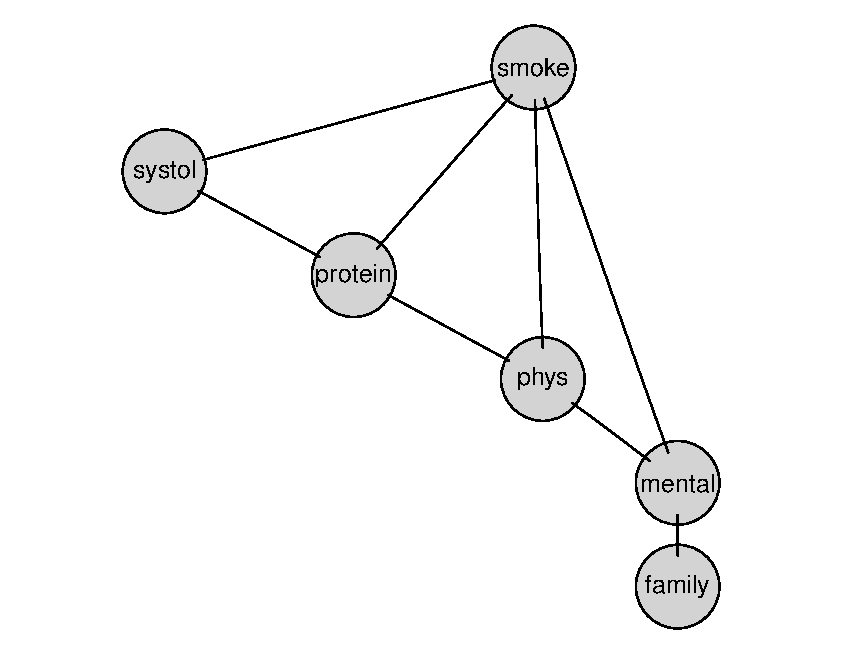
\includegraphics[scale=.3]{pics/reinis}\qquad\qquad 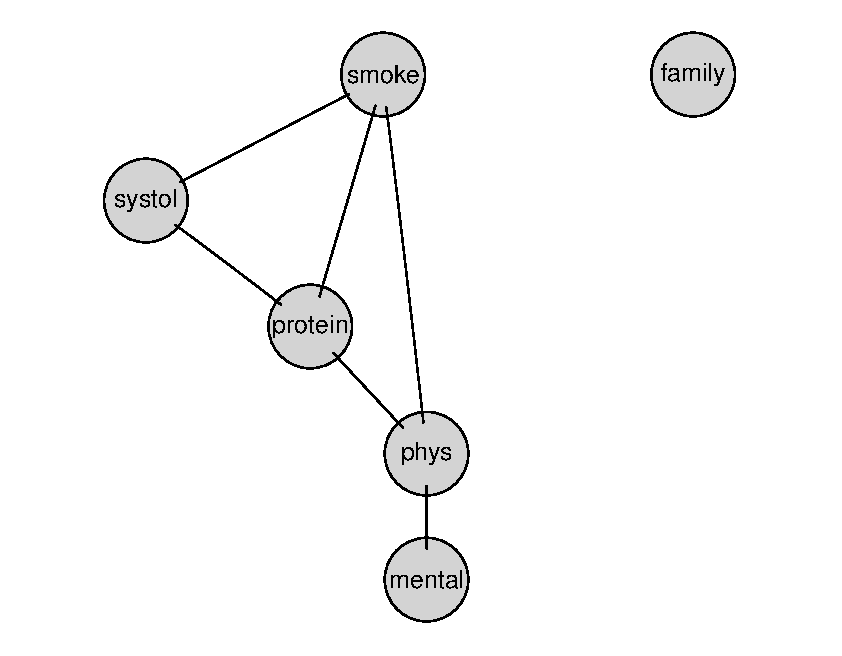
\includegraphics[scale=.3]{pics/reinis2}
\end{center}
\end{frame}

\begin{frame}{Modelling large data sets}
		\begin{beamercolorbox}[wd=\paperwidth,sep=3pt]{important}
With $>10$ variables stepwise methods are computationally prohibitive. 
	\end{beamercolorbox}
	\bigskip
	
Possible strategies:\\[.3cm]
\begin{enumerate}
	\item Use MCMC (\texttt{BDgraph} package)
	\item Focus on \alert{decomposable models} (\texttt{gRapHD} package).\\[.3cm]
	\item Rely on simpler models (e.g. pairwise interaction models). \\[.3cm]
	\item Restrict to very simple graphs (e.g. trees).
\end{enumerate}
\end{frame}

\begin{frame}[fragile,plain]{Bayesian Structure Learning using Birth-Death MCMC}
\texttt{bdgraph.mpl} in the package \texttt{BDgraph} can be used for discrete data. Consider the data table $X$ defined in Slide~\ref{DepAnx}.
\begin{lstlisting}
> install.packages("BDgraph"); library(BDgraph)
> X.fit <- bdgraph.mpl(X,method="dgm-binary",g.prior=.5)
> A <- X.fit$p_links+t(X.fit$p_links)
> qgraph::qgraph(A,layout="spring")
\end{lstlisting}
\begin{center}
	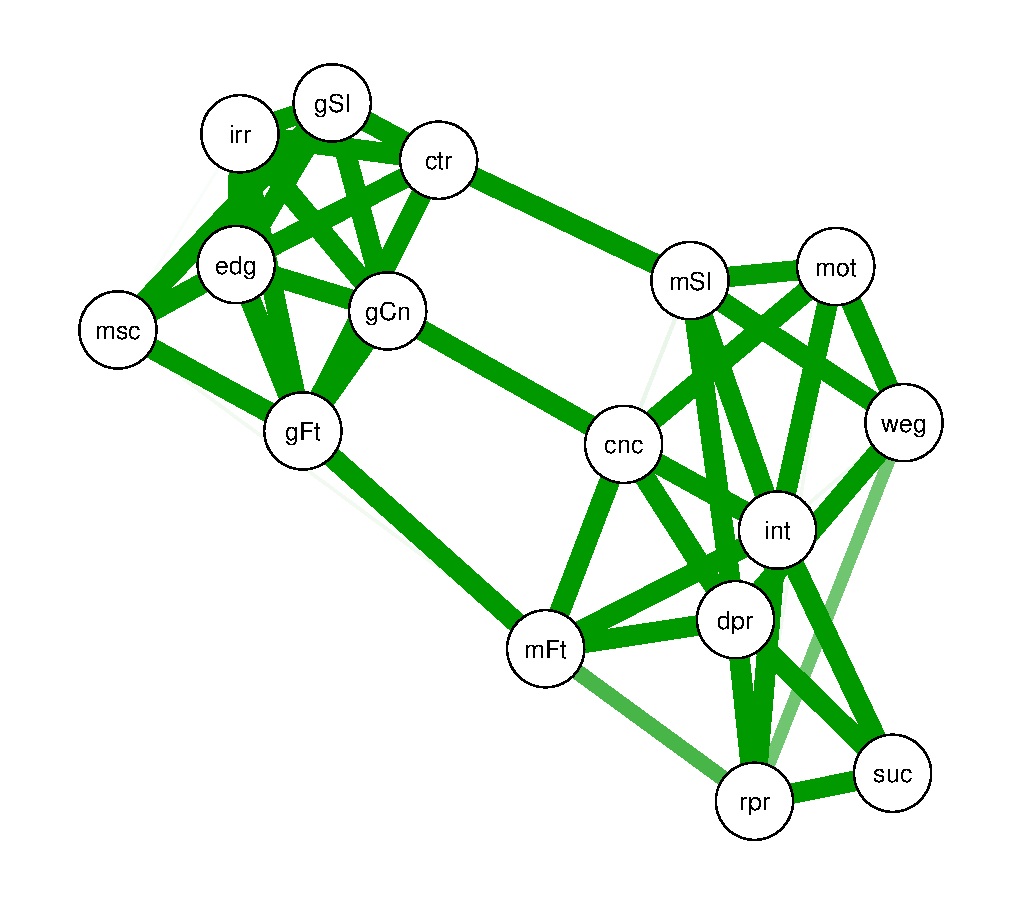
\includegraphics[scale=.4]{pics/BDgraphDA}
\end{center}
\end{frame}


\begin{frame}{Binary Ising model}
	Consider a log-linear model with only pairwise interactions.\\[.3cm]
	If $\cX=\{-1,1\}^m$ then $$f(x)\;=\;\tfrac{1}{Z(h,B)}\exp\left(\sum_i h_i x_i+\sum_{i<j}\beta_{ij}x_i x_j \right),$$
	where $h\in \R^m$ and $B=[\beta_{ij}]$ has zeros on the diagonal.\\[.3cm]
	Likelihood is hard to handle because $Z(h,B)$ is intractable if $m$ is large.\\
	\bigskip
	
	This will be our first encounter with pseudo-likelihood methods.
\end{frame}


\begin{frame}{Pseudo-likelihood approach}
\begin{alertblock}{Logistic regression}
Denoting \textcolor{blue}{$\eta_k=h_k+\sum_{i\neq k}\beta_{ik}x_i$}, the full conditional distributions satisfy
	$$
	\log p(x_k|x_{-k})=\eta_k x_k-\log(e^{-\eta_k}+e^{\eta_k })
	$$ 
	and so, if $p= p(1|x_{-k})$, then 
	$$
	\log \frac{p}{1-p}\;=\;2\eta_k\;=\;2h_k+\sum_{i\neq k}2\beta_{ik}x_i
	$$
\end{alertblock}
\begin{alertblock}{$\ell_1$-regularized logistic regression (Ravikumar et al, 2010)}
	Having observed $x^{(1)},\ldots,x^{(n)}$, to learn the support of $B$, we can optimize for each $k$ the logistic regression given the data. Alternatively we can maximize
	$$
	\sum_{i=1}^n \sum_{k\in V} \log p(x_k^{(i)}|x_{-k}^{(i)})\;-\;\lambda \|B\|_1.
	$$
\end{alertblock}
\end{frame}

\begin{frame}[fragile,label=DepAnx]{Using \texttt{IsingFit}}
	\begin{lstlisting}
> install.packages("IsingFit"); library(IsingFit)
> ncsdata=read.table(file="./data/DepressionAnxiety.txt") 
> colnames(ncsdata)=c("depr", "inte", "weig", "mSle", "moto", "mFat", "repr", "conc", "suic", "anxi", "even", "ctrl", "edge", "gFat", "irri", "gCon", "musc", "gSle") #Define variable names.
# remove two variables that are perfectly correlated with each other in the sample
> X <- (ncsdata[,-(10:11)])
# run the high-dimensional Ising model selection problem
> Res <- IsingFit(X,gamma = 0.5, plot=FALSE)
# compare with the correlation network
> lay <-averageLayout(Res$weiadj,cor(X), layout = "spring", repulsion = 1)
> qgraph(cor(X),layout=lay,labels=colnames(X))
> qgraph(Res$weiadj, layout = lay)
# both graphs appear on the next slide
\end{lstlisting}
For a discussion of this dataset see:\\[.2cm]
{\footnotesize Borsboom and Cramer, Network analysis: an integrative approach to the\\[-.2cm] structure of psychopathology, Annual review of clinical psychology, 9 (2013). }
\end{frame}


\begin{frame}{Two psychological disorders}
\alert{About the study:}\\[.5cm]
National Comorbidity Survey Replication  (NCS-R data)\\[.4cm]
9282 observations of 18 binary variables such as:\\
\texttt{depr} (Depressed mood), \texttt{inte} (Loss of interest), etc\\[.4cm]
These are symptoms related to two disorders:\\ major depression and generalized anxiety disorder.\\[.4cm]
Bridge variables: sleep problems, fatigue, and concentration problems.

\end{frame}


\begin{frame}{Two psychological disorders, continued}
\alert{About the data:}\\[.5cm]
Sparse contingency table: $872/65536$ nonzero cells. \\[.4cm]
5667 out of 9282 respondents recorded no symptoms.\\[.4cm]
two variables perfectly correlated with each other and other seven variables.\\[.4cm]
\end{frame}



\begin{frame}[label=depr_lasso]{}
	\begin{center}
		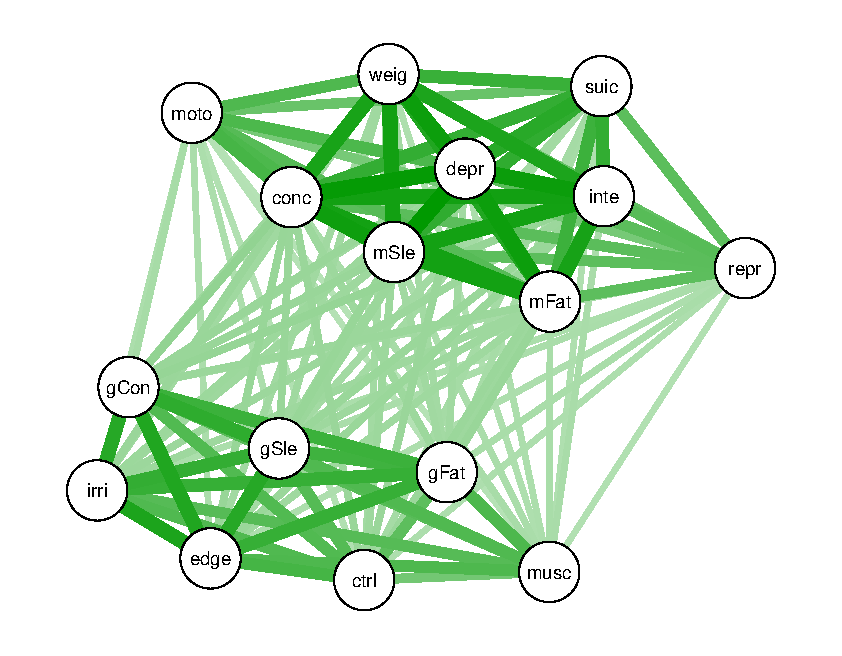
\includegraphics[scale=.5]{pics/depr_corr}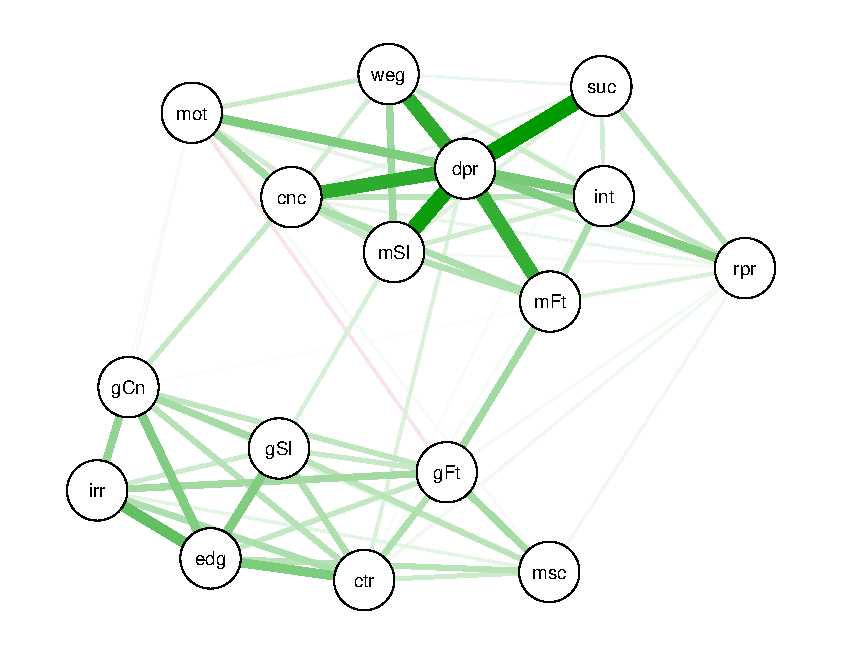
\includegraphics[scale=.5]{pics/depr_lasso}
	\end{center}
	Note that basically all edges on the right are green.
\end{frame}


\section{Beyond the standard set-up}

\begin{frame}[plain,noframenumbering]{}
\begin{center}
	{\Huge \textcolor{DarkRed}{Part 3: Beyond the standard set-up}}
\end{center}
\end{frame}

\begin{frame}{The ``standard'' set-up is not enough}
\begin{alertblock}{The standard set-up}
		\begin{itemize}
		\item Gaussian or log-linear models
		\item Likelihood or penalized likelihood inference.
	\end{itemize}
\end{alertblock}
\begin{alertblock}{Challenges}
	\begin{itemize}
		\item Heavy-tailed or multimodal and asymmetric data.
		\item Other types of misspecification.
		\item MLE computationally intractable.
		\item Models for \alert{mixed data} needed.
	\end{itemize}
\end{alertblock}
\begin{alertblock}{Useful \texttt{R} packages}
	\texttt{huge}: High-Dimensional Undirected Graph Estimation\\
	\texttt{smart}: Sparse Multivariate Analysis via Rank Transformation\\	
\end{alertblock}
\end{frame}

\begin{frame}{M-estimation}
	The MLE has some deficiencies (e.g. robustness, computational cost). \\[.3cm]
	\alert{M-estimators for a sample $X^{(1)},\ldots, X^{(n)}$}: A large family of alternatives.
	\begin{enumerate}
		\item $m_\theta:\cX\to \R$ a known function
		\item $\hat\theta$ maximizes $\frac{1}{n}\sum_{i=1}^n m_\theta(X^{(i)})$.
	\end{enumerate}
	
	Often M-estimators result in consistent estimators, which are asymptocially normal but in general less efficient.
	\begin{exampleblock}{Examples we saw:}
		\begin{itemize}
			\item Least Squares Estimator for Gaussian data is the the MLE solution. For non-gaussian data it is not but it provides an estimator with good statistical properties. 
			\item Penalized log-likelihood functions lead to M-estimators. 
			\item For the Ising model we can use conditional distributions to define a pseudo-likelihood. 
		\end{itemize}
	\end{exampleblock}
\end{frame}

\subsection{Some non-parametric approaches}

\begin{frame}[plain,noframenumbering]{}
\begin{center}
	{\huge \textcolor{DarkRed}{3.1 Some non-parametric approaches}}
\end{center}
\end{frame}

\begin{frame}{Pairwise interaction graphs}
	We first focus on models for which the density admits factorization
\begin{eqnarray*}
		p(x)&=&\frac{1}{Z(\psi)}\exp\Big(\underbrace{\sum_{ij\in E}\psi_{ij}(x_i,x_j)}_{\mbox{{\scriptsize interaction terms}}}+\underbrace{\sum_{i\in V}\psi_i(x_i)}_{\mbox{{\scriptsize main effects}}}\Big)\\
		&=&\prod_{ij\in E}\phi_{ij}(x_i,x_j)\prod_{i\in V}\phi_i(x_i).
\end{eqnarray*}
\begin{alertblock}{Main cases considered in the literature:}
	Semiparametric Exponential Family Graphical Models
\begin{itemize}
	\item $\psi_{ij}(x_i,x_j)=\beta_{ij}x_i x_j$, inference with $\ell_1$-regularized pseudo-likelihood.\end{itemize}
Gaussian Copula Models
\begin{itemize}
	\item $\psi_{ij}(x_i,x_j)=\beta_{ij}f_i(x_i) f_j(x_j)$ where $f_i$ are monotone functions.
\end{itemize}
\end{alertblock}\begin{beamercolorbox}[wd=\paperwidth,sep=5pt]{important}
	By Hammersley-Clifford, in both cases $X_i\indep X_j|X_{V\setminus \{i,j\}}$ if and only if $\beta_{ij}=0$.
\end{beamercolorbox}
\end{frame}

\begin{frame}{Semiparametric Exponential Family Graphical Models}
\begin{alertblock}{Yang, Ning, \& Liu (2018)}
	Semiparametric approach: $\psi_{ij}(x_i,x_j)=\beta_{ij}x_i x_j$ and $\psi_i(x_i)$'s kept general.\\[.3cm]
	$\beta_{ij}$'s are the parameters of interest and $\psi_i$ are \alert{nuisance} parameters. 
	\begin{alertblock}{Nuisance-free loss function}
	If $X,X'$ independent copies then
	$$
	\P\big(X=x,X'=x'|X_{-k}=x_{-k},X_{-k}'=x_{-k}',\{X_k,X_k'\}=\{x_k,x_k'\}\big)
	$$
does not depend on the normalizing constant nor on $\psi_k$.	\\[.2cm]	
This can be used to construct a pseudo-likelihood that depends only on $B$.		\end{alertblock}
Adding an $\ell1$-penalty term assure sparse solutions.
\end{alertblock}
\medskip 

Currently there is no \texttt{R} package; stay tuned. 
\end{frame}

\begin{frame}[label=npn]{Nonparanormal distributions}
	$(X_1,\ldots,X_m)$ has \textcolor{blue}{nonparanormal} distribution if $(f_1(X_1),\ldots,f_m(X_m))$ is Gaussian for some monotone functions $f_1,\ldots,f_m$.\\[.3cm]
	The functions $f_i$ are treated again as nuisance parameters. The correlation matrix is estimated directly using \textcolor{blue}{rank correlation statistics}:\\[.2cm]
	\begin{alertblock}{We can estimate the correlation matrix of $f(X)$ without knowing f!!}
		If $\tau_{ij}={\rm cor}(\sgn(X_i-X_i'),\sgn(X_j-X_j'))$ is the \textcolor{blue}{Kendall's tau statistic} then
	$$
	\Sigma^0_{ij}:={\rm cor}(f(X_i),f(X_j))\;=\;\sin\left(\tfrac{\pi}{2}\tau_{ij}\right).
	$$
	\begin{beamercolorbox}[wd=\paperwidth,sep=5pt]{goldbox}
	\begin{itemize}
		\item $\tau_{ij}$'s are invariant under monotone transformations on $X_i$'s.
		\item $f(X)$ is Gaussian and in this case the formula follows by standard results.
		\item the inverse $\Sigma^0$ holds the conditional independence structure of $X$.\\{\footnotesize ($f_i(X_i)\indep f_j(X_j)|{\rm rest}$ \qquad$\Leftrightarrow$\qquad $\beta_{ij}=0$ \qquad$\Leftrightarrow$\qquad $X_i \indep X_j|{\rm rest}$)}
	\end{itemize}
	\end{beamercolorbox}
	\end{alertblock}
\end{frame}


\begin{frame}[label=npn2]{Estimating nonparanormal graphical models}
		Compute \alert{Kendall's tau} coefficients from the data (c.f. Slide~\ref{tau}) 	$$
	\hat \tau_{ij}\;=\;\tfrac{1}{{n\choose 2}}\sum_{1\leq t\leq t'\leq n}{\rm sign}(X_{it}-X_{it'}){\rm sign}(X_{jt}-X_{jt'}).
	$$
	Define $\hat S^\tau=\sin(\tfrac{\pi}{2}\hat\tau_{ij})$.\\[.3cm]
	Concentration analysis based on U-statistics shows that
	$$
	\max_{ij}|\hat S^\tau_{ij}-\Sigma^0_{ij}|=\mathcal O\left(\sqrt{\tfrac{\log(mn)}{n}}\right).
	$$
	\begin{beamercolorbox}[wd=\paperwidth,sep=5pt]{important}
		Based on $\hat S^\tau$ we can now employ any standard Gaussian procedure to learn the graph, e.g., graphical lasso.
	\end{beamercolorbox}

\end{frame}

\begin{frame}[fragile]{Application using \texttt{huge} package}

{\small Stock market data: closing prices from all stocks in the S\&P 500 for all the days that the market was open between Jan 1, 2003 and Jan 1, 2008. }
	\begin{lstlisting}
> library(huge); data(stockdata) # Load the data 
> x = log(stockdata$data[2:1258,]/stockdata$data[1:1257,]) # Preprocessing 
> colnames(x) <- stockdata$info[,1]
> x.npn = huge.npn(x, npn.func="skeptic") # Nonparanormal + Kendal's tau
> out.npn = huge(x.npn,method = "glasso")
> plot(out.npn)
# plot the graph corresponding to lambda=0.397
> Khat <- (out.npn$icov[[15]]+t(out.npn$icov[[15]]))/2; colnames(Khat) <- rownames(Khat) <- colnames(x)
> dev.off(); qgraph::qgraph(-cov2cor(Khat),layout="spring")
	\end{lstlisting}
	This is a rather large example to be handled by \texttt{qgraph} directly.
	\begin{lstlisting}
> qgraph(x.npn,graph="glasso",sampleSize=nrow(x),layout="spring")
	\end{lstlisting}

	{\scriptsize Zhao, T., Liu, H., Roeder, K., Lafferty, J., \& Wasserman, L. (2012). The huge package for high-dimensional undirected graph estimation in R. Journal of Machine Learning Research.}
\end{frame}

\begin{frame}{}
The non-paranormal approach gives:
\begin{center}
	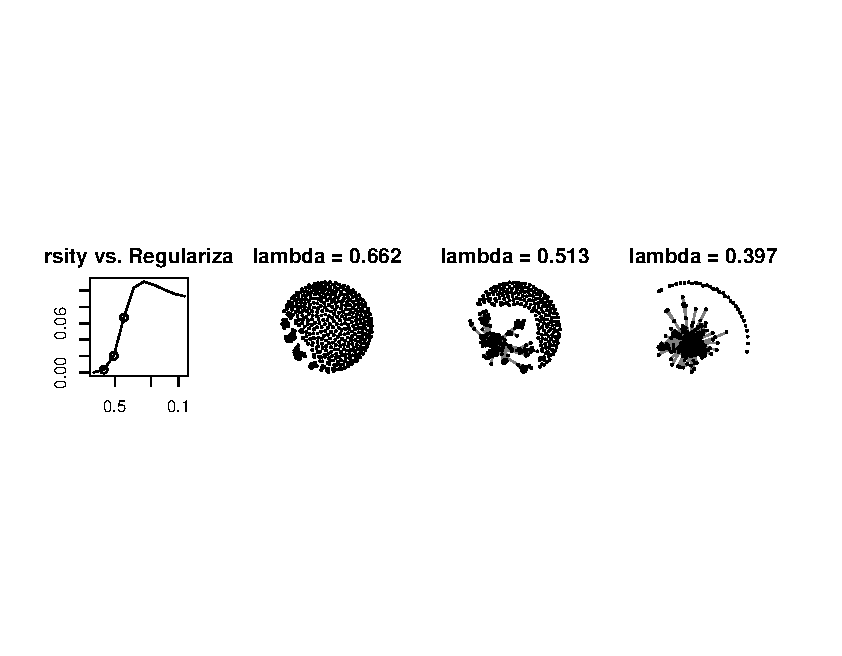
\includegraphics{pics/huge_stocks1}	
\end{center}
For comparison a direct Gaussian approach gives:
\begin{center}
	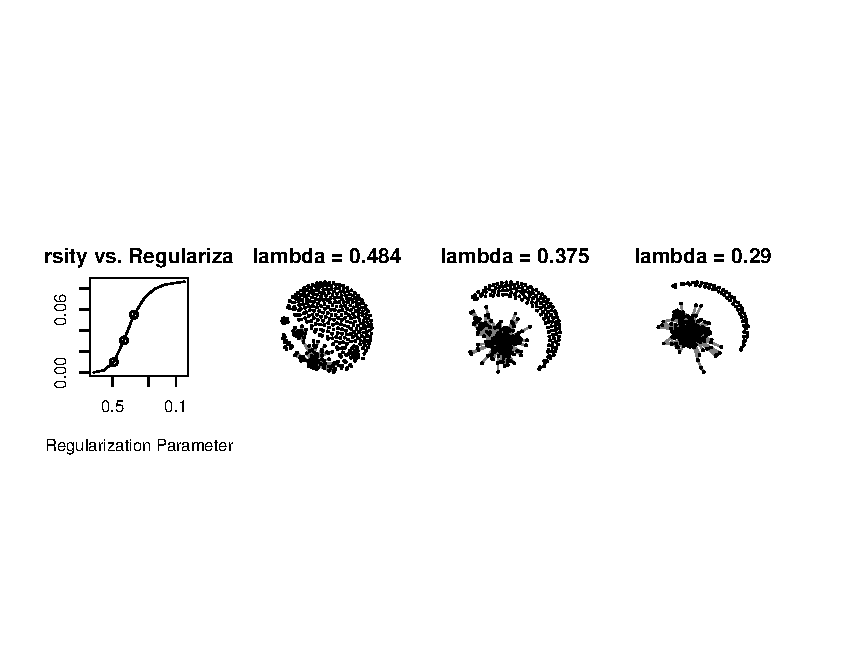
\includegraphics{pics/huge_stocks1_gauss}	
\end{center}
\end{frame}

\begin{frame}{}
\begin{center}
	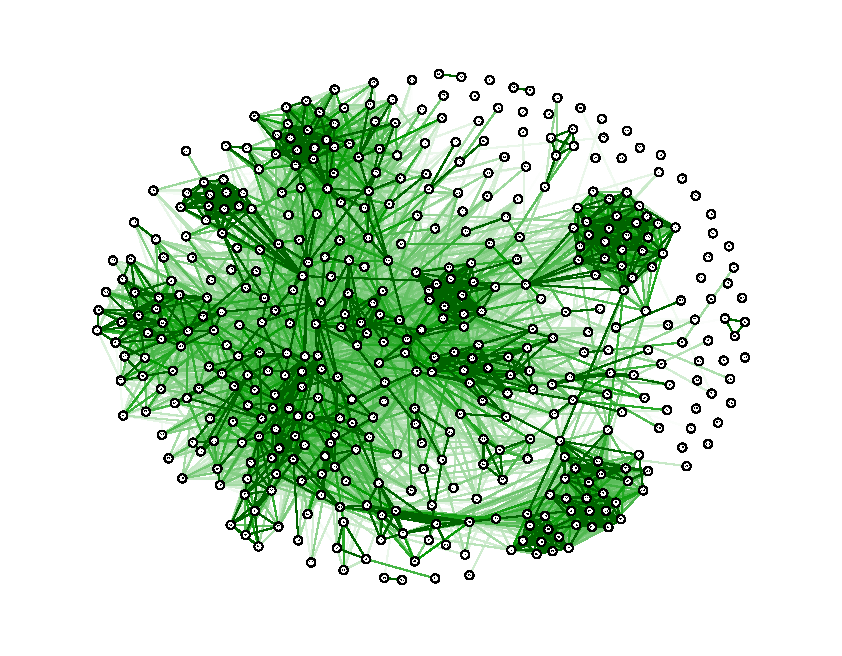
\includegraphics[scale=.8]{pics/huge_stocks2}	
\end{center}
Note that all edges are green.\\
{\scriptsize (for visualizing such big networks may be worthwhile to learn the \texttt{visNetwork} package)}
\end{frame}

\subsection{Partial correlation graph}

\begin{frame}[plain,noframenumbering]{}
\begin{center}
	{\huge \textcolor{DarkRed}{3.2 Partial correlation graphs}}
\end{center}
\end{frame}


\begin{frame}{Partial correlation graphs}
 \alert{Partial correlation graph}: $G=G(K)$ such that $ij\in E$ if and only if $K_{ij}\neq 0$.\\[.3cm] 
	Recall: For Gaussian variables the partial correlation graph is equal to the \alert{conditional independence graph}.\\[.3cm]
	If $X$ is not Gaussian, we still can be interested in the partial correlation graph.\\[.3cm]
	Simple idea: Still use $\ell_1$-regularized Gaussian likelihood which now acts as pseudo-likelihood. 
	\begin{itemize}
		\item This is a consistent estimator under minor conditions.
		\item We focus on scenarios where a better statistical analysis can be performed.
	\end{itemize}
\end{frame}


%\subsection{Transelliptical distributions}
%
%\begin{frame}[plain,noframenumbering]{}
%\begin{center}
%	{\huge \textcolor{DarkRed}{3.3 Transelliptical distributions}}
%\end{center}
%\end{frame}

\begin{frame}{Transelliptical distributions}
\begin{alertblock}{Elliptical distribution}
	$X=(X_1,\ldots,X_m)$ has an \textcolor{blue}{elliptical distribution} if its density function can be expressed as $$g((x-\mu)^T\Sigma^{-1}(x-\mu))$$
	for some $\mu\in \R^m$ and positive definite matrix $\Sigma$. \\[.2cm]
	e.g. multivariate Gaussian, multivariate t-distribution, Laplace distribution.
\end{alertblock}
\begin{alertblock}{Transelliptical distribution}
	$X$ has \textcolor{blue}{transelliptical} distribution if $(f_1(X_1),\ldots,f_m(X_m))$ has elliptical distribution for some monotone functions $f_1,\ldots,f_m:\R\to \R$: $$X\sim {\sc TE}(\Sigma_f; f_1,\ldots,f_m).$$
\end{alertblock}
\end{frame}

\begin{frame}{}
\begin{beamercolorbox}[wd=\paperwidth,sep=5pt]{result}
	The relation between Kendall's tau coefficient and the Spearman's rho given on Slide~\ref{npn} extends from the Gaussian to elliptical distributions.
\end{beamercolorbox}


$\bullet$ Compute $\hat \tau$ and $S^\tau$ as on Slide~\ref{npn2}.\\[.3cm]
$\bullet$ This results in a consistent estimator an a relatively small efficiency loss.
\bigskip

\begin{beamercolorbox}[wd=\paperwidth,sep=5pt]{important}
We follow the same procedure as nonparanormal distributions. Simply the interpretation of the output graph changes.	
\end{beamercolorbox}

For more details see: \\[.2cm]
{\footnotesize Liu, Han \& Zhang (2012). Transelliptical graphical models. In Advances in neural information processing systems.}\\[.2cm]

{\footnotesize Barber \& Kolar (2018). Rocket: Robust confidence intervals via Kendall's tau for transelliptical graphical models. The Annals of Statistics, 46(6B).}
%\begin{beamercolorbox}[wd=\paperwidth,sep=5pt]{notabene}
%	Intend to load manually from github the following functions in the \texttt{package}: \textcolor{black}{TCE.R}, \textcolor{black}{plot.TCE.R}, \textcolor{black}{smart.npn.R}.\\
%	Load from CRAN packages: \textcolor{black}{Matrix}, \textcolor{black}{pcaPP}, \textcolor{black}{igraph}.\\
%	Then the following code should run. 
%\end{beamercolorbox}
%
%\begin{lstlisting}
%> data(stockdata,package="huge")
%> x = log(stockdata$data[2:1258,]/stockdata$data[1:1257,]) # Preprocessing 
%> out.tel = TCE(x, method="kendall") # do the transelliptical thingy 
%> plot.TCE(out.tel)
%
%\end{lstlisting}
\end{frame}


	\begin{frame}[fragile]{Personality traits again}
	\begin{lstlisting}
> pers <- read.table("./data/personality0.txt")
> pers.npn = huge.npn(pers, npn.func="skeptic") # Nonparanormal 
# can be handled by qgraph directly
> qgraph(pers.npn,graph="glasso",sampleSize=nrow(pers),layout="spring")
\end{lstlisting}
	Compare with the direct lasso application on Slide~\ref{pers_lasso}.
	\begin{center}
		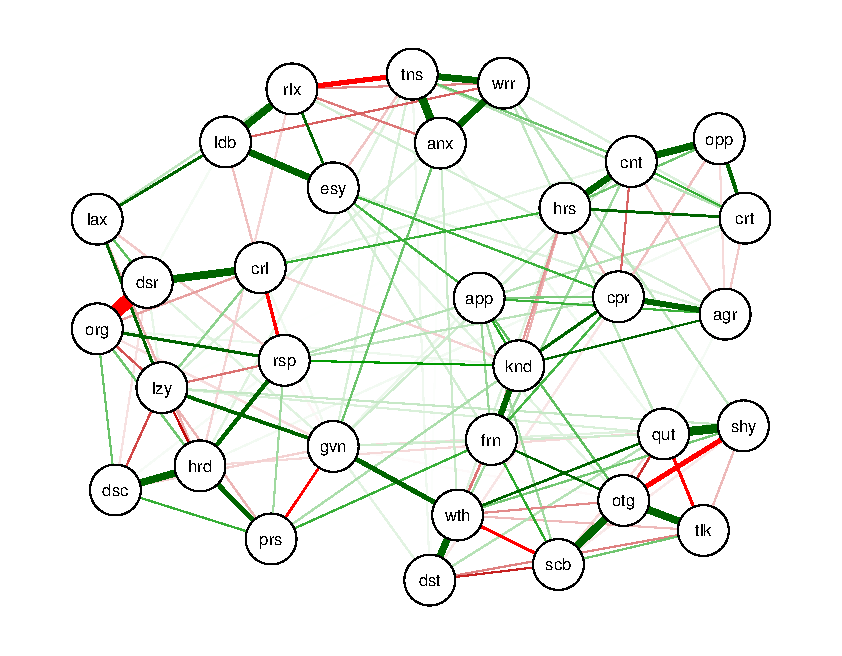
\includegraphics[scale=.6]{pics/pers_tel}
	\end{center}
\end{frame}

%	\begin{frame}[fragile]{Personality traits again}
%	\begin{lstlisting}
%> ncsdata=read.table(file="./data/DepressionAnxiety.txt") 
%> colnames(ncsdata)=c("depr", "inte", "weig", "mSle", "moto", "mFat", "repr", "conc", "suic", "anxi", "even", "ctrl", "edge", "gFat", "irri", "gCon", "musc", "gSle") #Define variable names.
%# remove two variables that are perfectly correlated with each other in the sample
%> X <- (ncsdata[,-(10:11)])
%> depr.npn = huge.npn(X, npn.func="skeptic") # Nonparanormal 
%# can be handled by qgraph directly
%> qgraph(depr.npn,graph="glasso",sampleSize=nrow(X),layout="spring")
%\end{lstlisting}
%	Compare with the direct lasso application on Slide~\ref{pers_lasso}.
%	\begin{center}
%		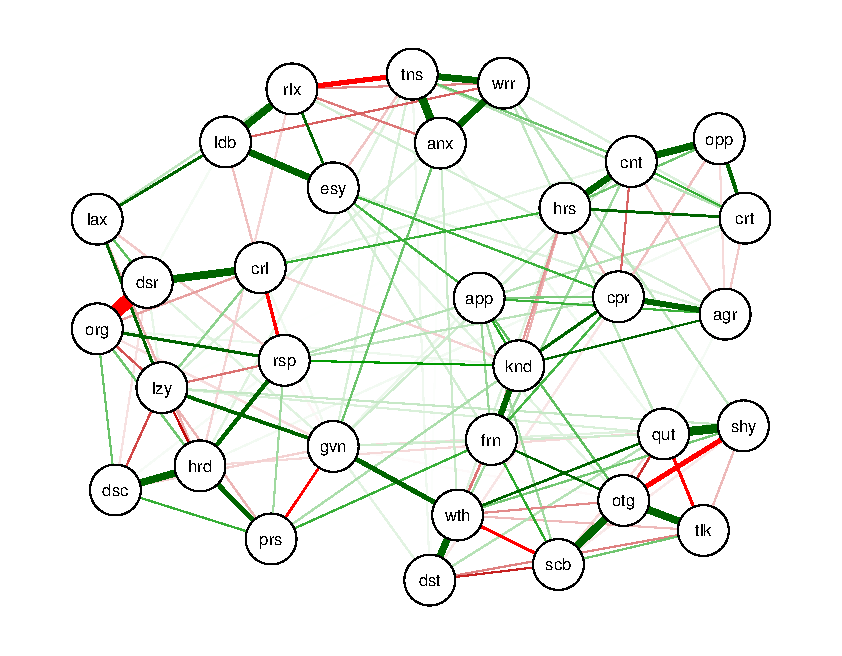
\includegraphics[scale=.6]{pics/pers_tel}
%	\end{center}
%\end{frame}


\end{document}

SEE PART 2

\section{Bayesian networks and causal discovery}

\begin{frame}[plain,noframenumbering]{}
\begin{center}
	{\Huge \textcolor{DarkRed}{Part 3: Bayesian networks and causal discovery}}
\end{center}
\end{frame}

\subsection{DAGs and their models}

\begin{frame}[plain,noframenumbering]{}
\begin{center}
	{\huge \textcolor{DarkRed}{3.1 DAGs and their models}}
\end{center}
\end{frame}

\begin{frame}{DAG terminology}
\textcolor{blue}{Directed acyclic Graph (DAG)} is a directed graph with no directed cycles.\\[.2cm]
Equivalently, we can order the vertices so that an arrow always goes from smaller to larger vertex.\\[.2cm]
	\alert{parents $\pa(v)$}: nodes $u$ such that $u\to v$ in $G$,\\[.3cm]
	directed path $u\to \cdots \to v$,\\[.3cm]
	path $u\leftrightarrow \cdots \leftrightarrow v$,\\[.3cm]
	\alert{descendants ${\rm de}(v)$} all nodes $u$ s.t. there is a directed path from $v$ to $u$,\\[.3cm]
	\alert{non-descendants $\nd(v)$}: all the other nodes in $V\setminus \{v\}$.\\[.3cm]
	\alert{$v$-structure}: induced subgraph of the form $u\to w\leftarrow v$
\end{frame}

\begin{frame}{Example}
	\begin{center}
		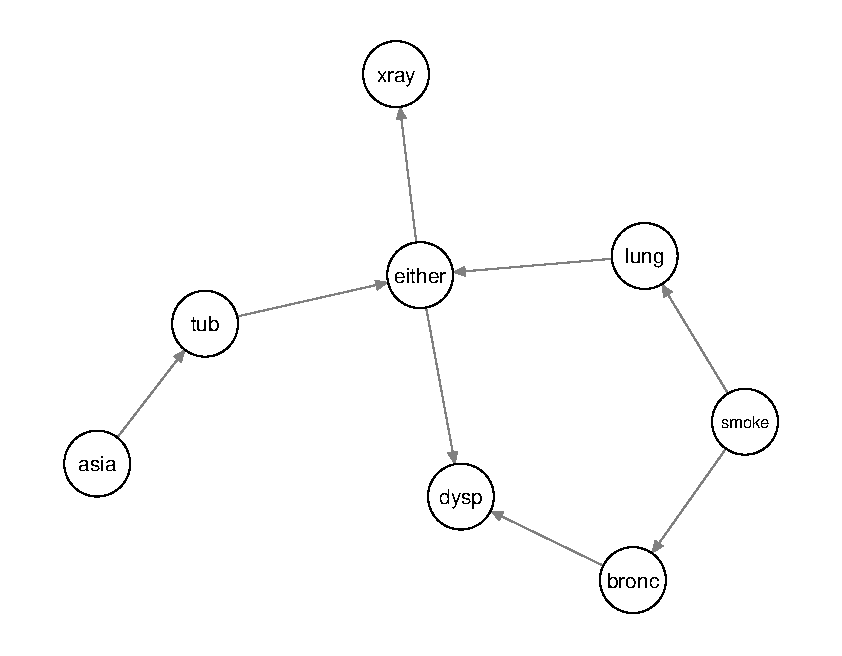
\includegraphics[scale=.6]{pics/chestdag}
	\end{center}
	Give an example of a v-structure. What are the parents of \texttt{either}? Is there a directed path from \texttt{bronc} to \texttt{xray}? Who are the descendants of \texttt{asia}? Who are the non-descendants?
\end{frame}

\begin{frame}[fragile]{d-separation}
	A path $\pi$ from $u$ to $v$ is \alert{blocked} by $S\subset V$ if $\pi$ contains one of the following types of nodes:
	\begin{itemize}
		\item a node $v\in S$ such that the path looks locally like $\to v\to $, $\leftarrow v\leftarrow$, or $\leftarrow v\to$.
		\item  a node $v\notin S$ such that $S\subseteq \nd(v)$ and the path looks locally like $\to v\leftarrow$.
	\end{itemize} 
	\bigskip
	
	Two subsets $A$ and $B$ are said to be \alert{d-separated} by $S$ if all chains from $A$ to $B$ are blocked by $S$.
	
	\medskip 
	Package \texttt{bnlearn} has a function \texttt{dsep}:
\begin{lstlisting}
> library(bnlearn)
> chestdag = model2network("[asia][tub|asia][smoke][lung|smoke][bronc|smoke][either|lung:tub][xray|either][dysp|bronc:either]")
> dsep(chestdag, "asia", "xray", c("lung","bronc"))	
[1] FALSE
\end{lstlisting}
[Mention hierarchical layouts]
\end{frame}

\begin{frame}{DAG models/Bayesian networks}
	Let $G$ be a directed acyclic graph (DAG).\\
	We say that $f(\bs x)$ factorizes according to $G$ if for all $\bs x\in \cX$
	$$
	f(\bs x)\;=\;\prod_{v\in V}f(x_v|\bs x_{{\rm pa}(v)}).
	$$
%	\begin{alertblock}{Chain rule in probability} 
%	For any ordering of the nodes in $V$ we have
%	$$f(\bs x)=f_{v_1}(x_{v_1})f_{v_2|v_1}(x_2|x_1)\cdots f_{v_m|V\setminus m}(x_{v_m}|x_{V\setminus m}).$$
%	\end{alertblock}
%	\vspace{-.5cm}
%	\begin{alertblock}{Important reformulation of conditional independence} 
%$i\indep j|C$ \quad if\quad  
%	$f_{i|C\cup j}(x_i|\bs x_{C\cup j})=f_{i|C}(x_i|\bs x_{C}).$
%	\end{alertblock}
%	\medskip
\begin{beamercolorbox}[wd=\paperwidth,sep=5pt]{important}
	Factorization is equivalent to any of the following Markov properties:
	\begin{itemize}
		\item [(G)] $A\indep B|S$ whenever $S$ d-separates $A$ and $B$.
		\item [(L)] $v\indep \nd(v)|\pa(v)$ for every $v\in G$.
	\end{itemize}
	This results holds with no restrictions on the support of $f$.
\end{beamercolorbox}	
\medskip
We reiterate: $i\indep j|S$ if and only if $S$ \alert{d-separates} $i$ and $i$ in $G$.
\end{frame}

%\begin{frame}{Hierarchical layout}
%ichestdag <- igraph.from.graphNEL(as.graphNEL(chestdag))
%dag <- toVisNetworkData(ichestdag)
%visNetwork(dag$nodes,dag$edges) %>% 
%visEdges(arrows = "from") %>% 
%visHierarchicalLayout() # same as   visLayout(hierarchical = TRUE) 
%\end{frame}

\begin{frame}[fragile]{Belief propagation and inference}
	Belief propagation provides a computationally efficient way to compute various marginal and conditional distributions for a DAG model.\\[.2cm]
First we set up some distribution by specifying terms of the factorization.
	\begin{lstlisting}
library(gRain)
yn <- c("yes","no")
a <- cptable(~asia,values=c(1,99),levels=yn)
t.a <- cptable(~tub+asia,values=c(5,95,1,99),levels=yn)
s <- cptable(~smoke,values=c(5,5),levels=yn)
l.s <- cptable(~lung+smoke,values=c(1,9,1,99),levels=yn)
b.s <- cptable(~bronc+smoke,values=c(6,4,3,7),levels=yn)
e.lt <- cptable(~either+lung+tub,values=c(1,0,1,0,1,0,0,1),levels=yn)
x.e <- cptable(~xray+either,values=c(98,2,5,95),levels=yn)
d.be <- cptable(~dysp+bronc+either,values=c(9,1,7,3,8,2,1,9),levels=yn)
plist <- compileCPT(list(a,t.a,s,l.s,b.s,e.lt,x.e,d.be))
grn1 <- grain(plist)
grn1c <- compile(grn1)
grn1c <- propagate(grn1c)
	\end{lstlisting}
\end{frame}


\begin{frame}[fragile]{}
		To compute various joint distributions and conditional distributions of a variable given a subset of variables we run.
\begin{lstlisting}
> querygrain(grn1c,nodes=c("lung","bronc"),type="joint")
     bronc
lung     yes     no
  yes 0.0315 0.0235
  no  0.4185 0.5265
  
> querygrain(grn1c,nodes=c("dysp","asia"),type="conditional")
     dysp
asia        yes        no
  yes 0.4501375 0.5498625
  no  0.4358275 0.5641725
\end{lstlisting}
We can also see what happens when we fix values of some variables. 
\begin{lstlisting}
> grn1c.ev <- setFinding(grn1c,nodes=c("asia","smoke"),states=c("yes","yes"))
> querygrain(grn1c.ev,nodes=c("lung","bronc"),type="joint")
     bronc
lung   yes   no
  yes 0.06 0.04
  no  0.54 0.36
\end{lstlisting}

\end{frame}

\begin{frame}[fragile]{Learning distributions from data}
In some special situations the DAG structure can be specified by an expert.\\[.3cm]

	Given data we can then learn the underlying conditional probabilities.
	\begin{lstlisting}
> data("chestSim500",package='gRbase')
> simdagchest <- grain(as.graphNEL(chestdag),data=chestSim500)
> simdagchest <- compile(simdagchest,propagate=TRUE,smooth=.1)
> querygrain(simdagchest,nodes=c("lung","bronc"),type="joint")
     bronc
lung         yes         no
  yes 0.02539682 0.02060318
  no  0.42860318 0.52539682	
 \end{lstlisting}
	Then inference can be made as explained earlier.
\end{frame}


\begin{frame}[fragile]{Learning the graph}
Learning the underlying DAG from the data is the major problem. \\[.3cm]

\begin{beamercolorbox}[wd=\paperwidth,sep=5pt]{result}
Important links:\\[.2cm]
\textcolor{blue}{\url{annehpetersen.shinyapps.io/causalDisco/}} -- an overview of available methods to learn DAGs in \texttt{R}.	\\[.1cm]
\textcolor{blue}{\url{www.bnlearn.com}} -- an overview of methods in \texttt{bnlearn}.	
	\end{beamercolorbox}

\begin{alertblock}{Example: Coronary artery disease data}
	A cross classified table with observational data from a Danish heart clinic. The response variable is CAD:
	\begin{lstlisting}
data(cad1,package='gRbase')
cad.bn <- hc(cad1)
qgraph::qgraph(cad.bn)
\end{lstlisting}
\end{alertblock}
\end{frame}

\begin{frame}{}
\begin{center}
	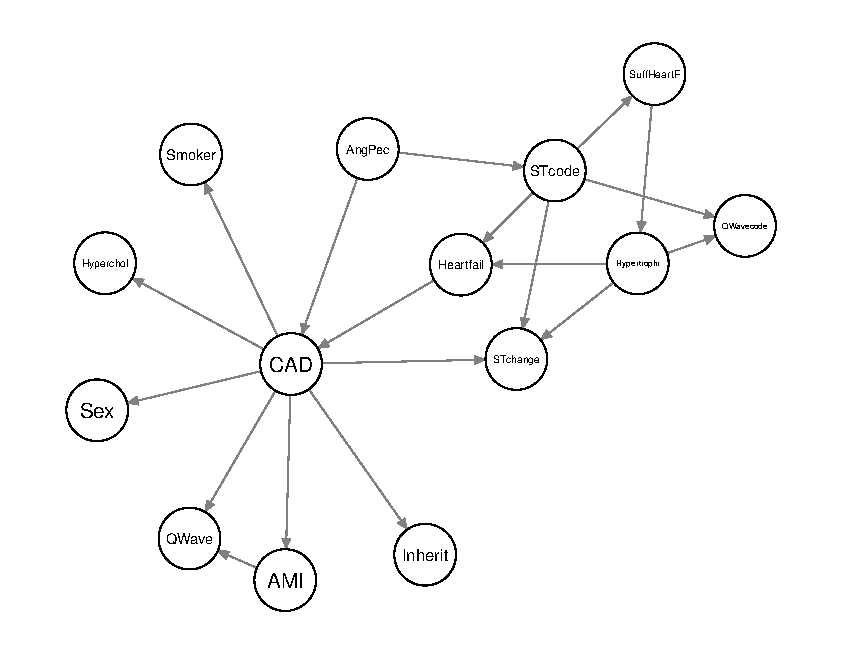
\includegraphics[scale=.7]{pics/cad_hc}
\end{center}
	It is important to incorporate prior knowledge. 
See \url{http://www.bnlearn.com/examples/whitelist/} for details.
\end{frame}

\begin{frame}{}
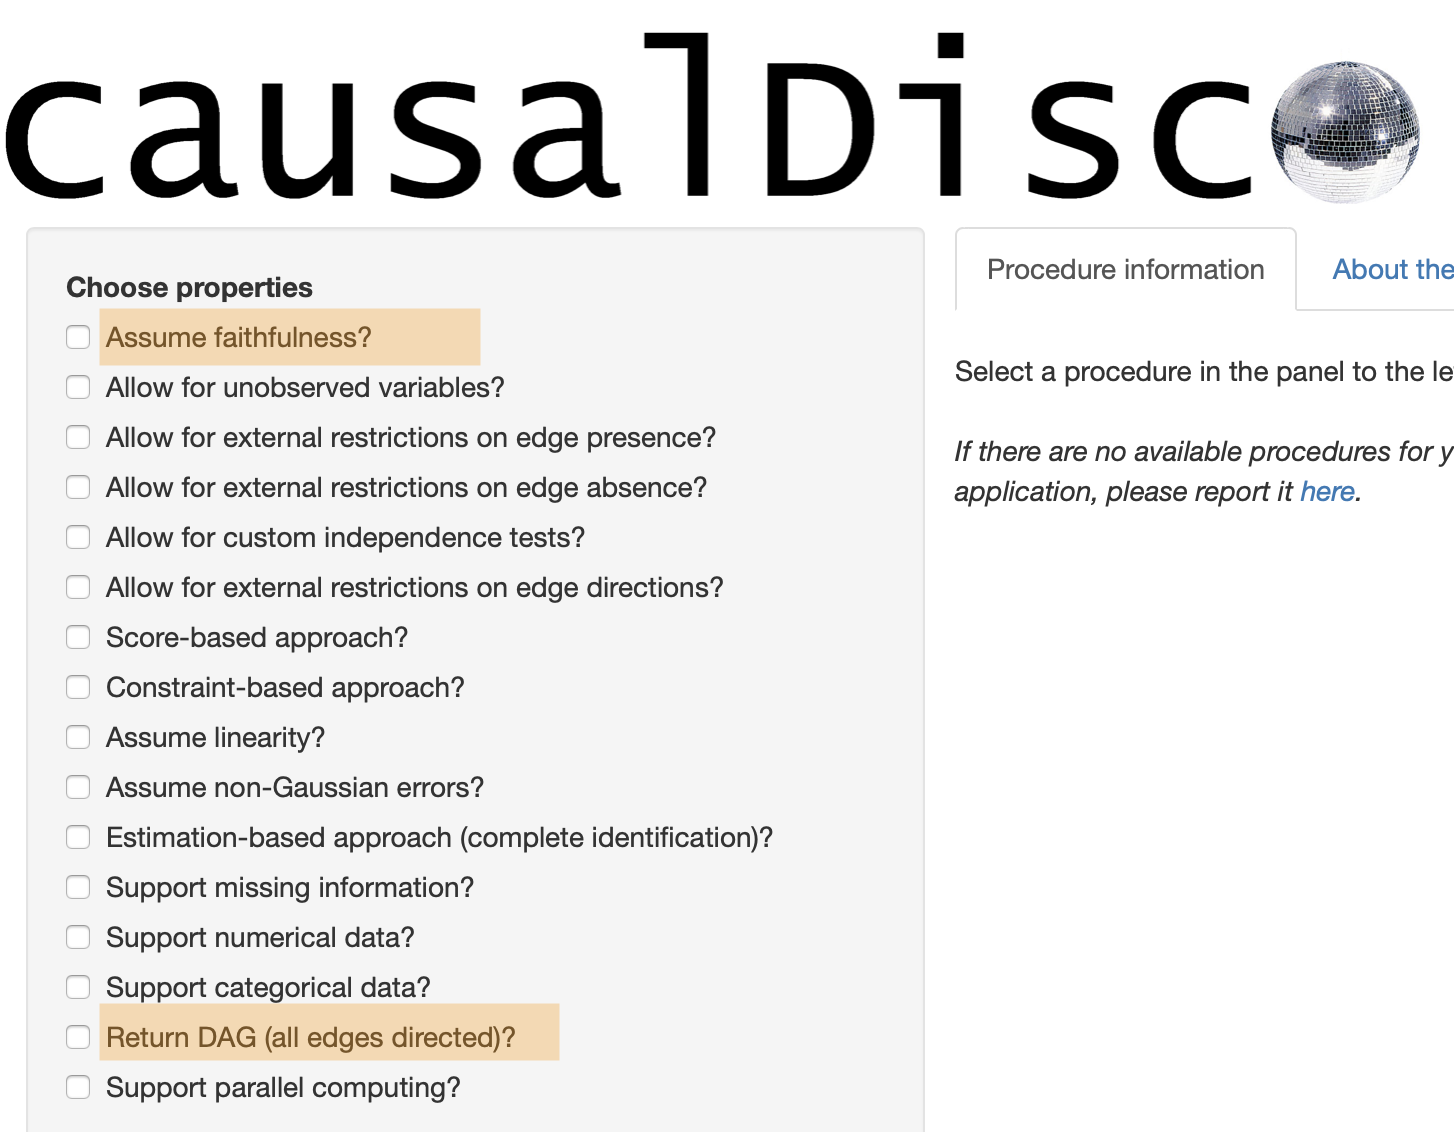
\includegraphics[scale=.4]{pics/causalDisco_marked}	
\end{frame}

\begin{frame}{Faithfulness}
	If $f$ factorizes with respect to the DAG $G$ then
	$$
	S \mbox{ d-separates }A \mbox{ and }B \mbox{ in }G \qquad\Longrightarrow\qquad A\indep B|S.
	$$
	At least in principle, $f$ may satisfy some additional conditional independence statements so the reverse implication may not hold. \\[.3cm]
	$f$ is \alert{faithful} to the DAG $G$ if 
	$$
	S \mbox{ d-separates }A \mbox{ and }B \mbox{ in }G \qquad\Longleftrightarrow\qquad A\indep B|S.
	$$
	\smallskip 
	
	This assumption is not entirely innocent:\\
	{\scriptsize Uhler, C., Raskutti, G., B\"{u}hlmann, P., \& Yu, B. (2013). Geometry of the faithfulness assumption in causal inference. The Annals of Statistics.}
\end{frame}

\begin{frame}{PC algorithm}
Currently one of the most popular algorithms.
	\begin{alertblock}{Stage one: Learn the skeleton.}
Use the fact that \qquad $u\not\sim v\quad\Longleftrightarrow\quad \exists S\subseteq V\mbox{ s.t. }u\indep v|S$.\\[.2cm]
 {\small Starting with the complete graph, conditional independences with an increasing order are tested and edges are removed.}
\end{alertblock}
	\begin{alertblock}{Stage two: Learn the edge directions.}
Several algorithms are implemented in \texttt{pcalg}
\end{alertblock}
\end{frame}

\begin{frame}[fragile]{Application for CAD data}
We use part of the CAD data to obtain a data set of binary variables.
	\begin{lstlisting}
library(pcalg); library(gRbase)
# use again the CAD dataset. remove one non-binary variable
cad <- data.matrix(cad1)-1; 
 \end{lstlisting}
Run the PC algorithm with the implemented discrete independence test.
	\begin{lstlisting}
suffStat <- list(dm=cad,nlev=rep(2,14)+diag(14)[2,],adaptDF=TRUE)
# m.max=4 because there is not enough data to set for bigger conditioning sets
cad.bn <- pc(suffStat,disCItest,alpha=0.1,labels=colnames(cad),m.max=4)
qgraph::qgraph(cad.bn)
 \end{lstlisting}
The package has also implemented testing CI for binary distributions (function \texttt{binCItest}) and also any external function can be called here.
\begin{itemize}
	\item may be important in case of small sample sizes as in the example above.
\end{itemize}
\end{frame}

\begin{frame}{Markov equivalence}
Only very rarely we can identify the underlying DAG from \textcolor{blue}{observational data}.\\[.2cm] 
\begin{beamercolorbox}[wd=\paperwidth,sep=5pt]{important}
	DAGs can be learned only up to some equivalence class.
\end{beamercolorbox}
\smallskip 
	e.g.\quad $\overset{1}{\bullet}\to \overset{2}{\bullet}$, $\overset{1}{\bullet}\leftarrow \overset{2}{\bullet}$, and $\overset{1}{\bullet}- \overset{2}{\bullet}$ all define the same model.\\[.2cm]
	
\begin{beamercolorbox}[wd=\paperwidth,sep=5pt]{result}	Two DAGs are \textbf{Markov equivalent} (define the same statistical model) if and only if they have the same skeleton and v-structures.
\begin{itemize}
	\item \alert{Essential graph} describes the Markov equivalence class. 
\end{itemize}
\end{beamercolorbox} 
\smallskip
\begin{beamercolorbox}[wd=\paperwidth,sep=5pt]{important}
	In certain scenarios there is a way around this, which we will discuss:
	\begin{itemize}
		\item Use interventions (experimental economics?)
		\item Instead of a DAG, assume an underlying Structural Causal Model.
	\end{itemize}
\end{beamercolorbox}
\end{frame}

\begin{frame}[fragile]{Visualize the essential graph}
\begin{lstlisting}
library(ggm)
qgraph::qgraph(as(essentialGraph(amat(chestdag)),"graphNEL"))
\end{lstlisting}
\begin{center}
	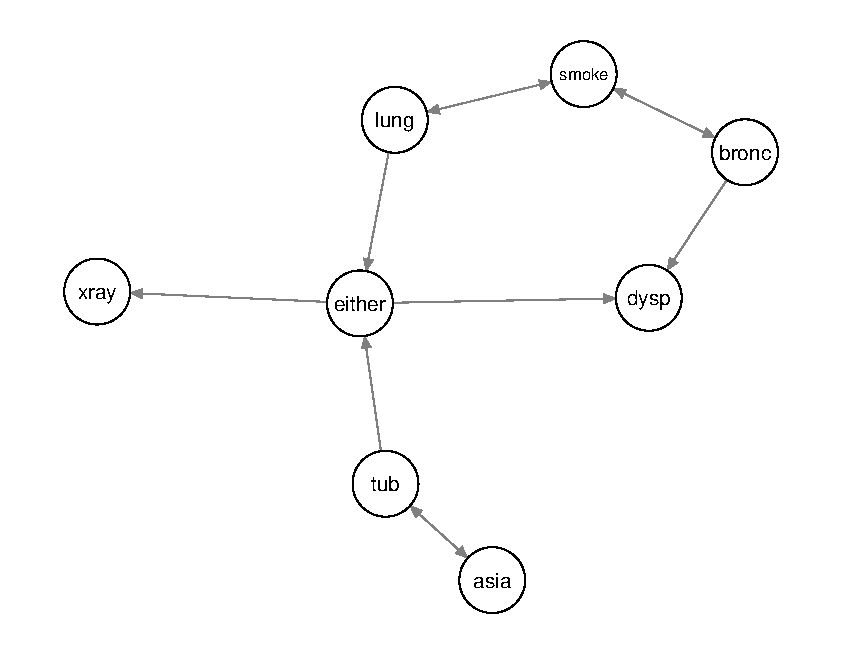
\includegraphics[scale=.6]{pics/chestdag_equiv}
\end{center}
\end{frame}

\subsection{Structural causal models}

\begin{frame}[plain,noframenumbering]{}
\begin{center}
	{\huge \textcolor{DarkRed}{3.2 Structural Causal Models}}
\end{center}
\end{frame}

\begin{frame}[fragile,label=SCM]{Structural Causal Models}
	A structural causal model (SCM) consists of a collection of $m$ structural assignments
	$$
	X_i\;:=\;f_i(\pa_i,\epsilon_i)\qquad\mbox{for }i=1,\ldots,m,
	$$
	where $\pa_i\subset \{X_1,\ldots,X_m\}\setminus \{X_i\}$ and all $\epsilon_i$ are independent of each other. \\[.2cm]
	The underlying graph $G$ of an SCM is defined in the obvious way.
	\begin{alertblock}{If $G$ is a DAG, sampling data from SCMs is easy}
		Sample from the SCM: $X_1=X_3^2+\epsilon_1$, $X_2=\sin(X_3)+\epsilon_2$, $X_3=\epsilon_3$, $X_4=X_2+e^{X_3+\epsilon_4}$, with $\epsilon_i$ having respectively normal, chi-squared, uniform, and normal distribution.  
		\begin{lstlisting}
set.seed(1); n <- 100
X3 <- runif(n)-0.5
X1 <- X3^2+rnorm(n)
X2 <- sin(X1)+rnorm(n)^2
X4 <- X2+exp(X3+rnorm(n))
X <- cbind(X1,X2,X3,X4)
\end{lstlisting}
	\end{alertblock}
\end{frame}

\begin{frame}[fragile]{Gaussian DAG models}
\begin{alertblock}{Linear Structural Equation models}
	Let $\varepsilon_1, \ldots,\varepsilon_m$ be independent variables. Consider a model
		$$
		X_i \;=\;\sum_{j\in {\rm pa}(i)}\lambda_{ij}X_j\;+\;\varepsilon_i.
		$$
\end{alertblock}
\begin{beamercolorbox}[wd=\paperwidth,sep=2pt]{important}
The \textcolor{SeaGreen}{Gaussian DAG models} are precisely the Linear Structural Equation models on DAGs, where $\epsilon_i$ are independent Gaussian variables.
\end{beamercolorbox} 
The function \texttt{fitDag} in the \textbf{ggm} package fits Gaussian DAGs.
	\begin{lstlisting}
> library(ggm)
> gdag1 <- DAG(LeanMeat~Meat13:Fat11:Fat12, Meat13~Meat11:Meat12,Fat12~Fat11,Fat13~Meat11:Meat12,Meat12~Meat11)
> qgraph::qgraph(as(gdag1,"graphNEL")).  # to visualize the DAG
> fdag1 <- fitDag(gdag1, S.carc,nrow(carcass))
> fdag1$dev. # the deviance is really large and the p-value is basically 0.
[1] 552.2726
	\end{lstlisting}
\end{frame}

\begin{frame}[fragile]{Interventions}
Recall: Typically impossible to identify the DAG from observational data. 	\\[.3cm]
Things are better if we can observe the system under \alert{intervention} or  include the domain knowledge.\\[.3cm]
We consider only the simplest way to intervene by fixing a value of a variable. 

\medskip
Consider the example on Slide~\ref{SCM} with $X_2 \leftarrow 1$
\begin{lstlisting}
set.seed(1); n <- 100
X3 <- runif(n)-0.5
X1 <- X3^2+rnorm(n)
X2 <- 1
X4 <- X2+exp(X3+rnorm(n))
X <- cbind(X1,X2,X4)
\end{lstlisting}

The distribution of $(X_1,X_3)$ did not change!
\end{frame}

\begin{frame}[fragile]{}
\begin{lstlisting}
scm = model2network("[X3][X1|X3][X2|X1][X4|X2:X3]")
bnlearn::dsep(scm, "X2", "X3","X1")	
qgraph::qgraph(essentialGraph(amat(scm)))
\end{lstlisting}
There are two DAGs Markov equivalent to the DAG of this SCM.
\begin{center}
	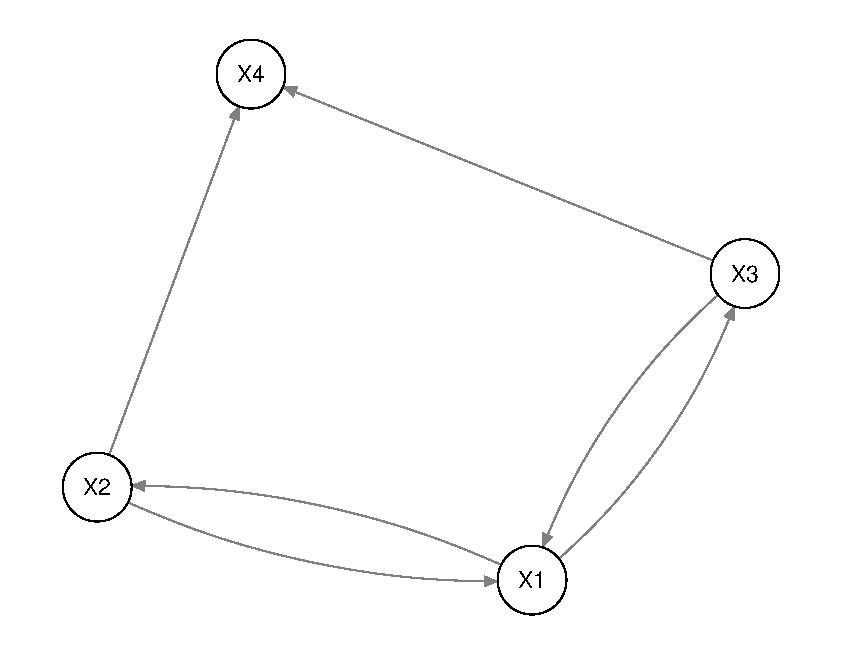
\includegraphics[scale=.4]{pics/scm_essential}
\end{center} 
In one of them the distribution of $X_1$ under $X_2\leftarrow 1$ changes. Intervening on $X_3$ allows us to pin down the original DAG. 
\end{frame}

%\begin{frame}{Topics we omit	}
%	Many different types of graphical models are used.
%	\begin{enumerate}
%		\item undirected graphical models (aka Markov random fields)
%		\item models of DAGs (aka Bayesian Networks)
%		\item chain graph models
%		\item mixed graph models
%		\item  
%	\end{enumerate}
%\end{frame}

%\subsection{Causality}

%\begin{frame}[plain,noframenumbering]{}
%\begin{center}
%	{\Huge \textcolor{DarkRed}{4. Causality}}
%\end{center}
%\end{frame}
%
%\begin{frame}{Association versus causation}
%	gg
%\end{frame}

\begin{frame}{More on learning the DAG}
\begin{beamercolorbox}[wd=\paperwidth,sep=5pt]{important}
If $X$ is induced by a Structural Causal Model with graph $G$ then $X$ satisfies the Markov properties with respect to $G$. The model is often strictly smaller	than the underlying DAG model, which allows for graph identification. 
\end{beamercolorbox}

Some cases when identification is possible:
\begin{itemize}
	\item In linear models if $\varepsilon$ are non-Gaussian, the DAG can be recovered. (\alert{LiNGAM})
	\item Additive noise models ($X_i=f_i(X_{\pa(i)})+\epsilon_i$)
\end{itemize}
\end{frame}

\begin{frame}[fragile]{LiNGAM in action}
	Package \texttt{CompareCausalNetworks} provides a unified interface for the estimation of causal networks that includes a handful of available methods (also LiNGAM).\\[.3cm]
		\begin{lstlisting}
library(CompareCausalNetworks)
# use again the CAD dataset. remove one non-binary variable
data(cad1,package='gRbase')
cad <- data.matrix(cad1)-1; 
g.cad <- getParents(cad, method="LINGAM") # learn the DAG
qgraph::qgraph(g.cad)
 \end{lstlisting}

\end{frame}

%\end{document}

\section{GMs with latent variables}

\begin{frame}[plain,noframenumbering]{}
\begin{center}
	{\Huge \textcolor{DarkRed}{4. GMs with latent variables}}
\end{center}
\end{frame}

%\begin{frame}{Idea}
%	Partial correlations allow to measure association between random variables with the effect of potentially confounding variables removed. \\
%	However, if the confounding variables are unobserved, or are simply not included the data set, this will not work. 
%\end{frame}

\begin{frame}{What is a hidden variable?}
	Random vector $Y=(X,H)$: $X$ observed, $H$ \alert{hidden/latent}. \\[.3cm]
	Observing $X$, we only get information about the marginal $p_X$.\\[.3cm]
	Since $p(x)=\sum_h p(h)p(x|h)$, sometimes $p(x)$ may be enough to recover $p(x,h)$.
	\begin{exampleblock}{Examples}
		Factor analysis models, hidden Markov models, Markov switching models, mixture models, latent tree models.
	\end{exampleblock}
\end{frame}


\begin{frame}{Simpson's paradox}
%	Two real-valued random variables  $X$ and $Y$ are \alert{positively associated} if ${\rm cov}\{f(X),g(Y)\}\geq 0$ for all $f$, $g$ which are non-decreasing.

%\pause

\alert{The Yule-Simpson paradox} says that we may have $X$ and $Y$ positively associated but $X$ and $Y$ negatively associated conditionally on a third variable $Z$. \\[.3cm]
\begin{center}
	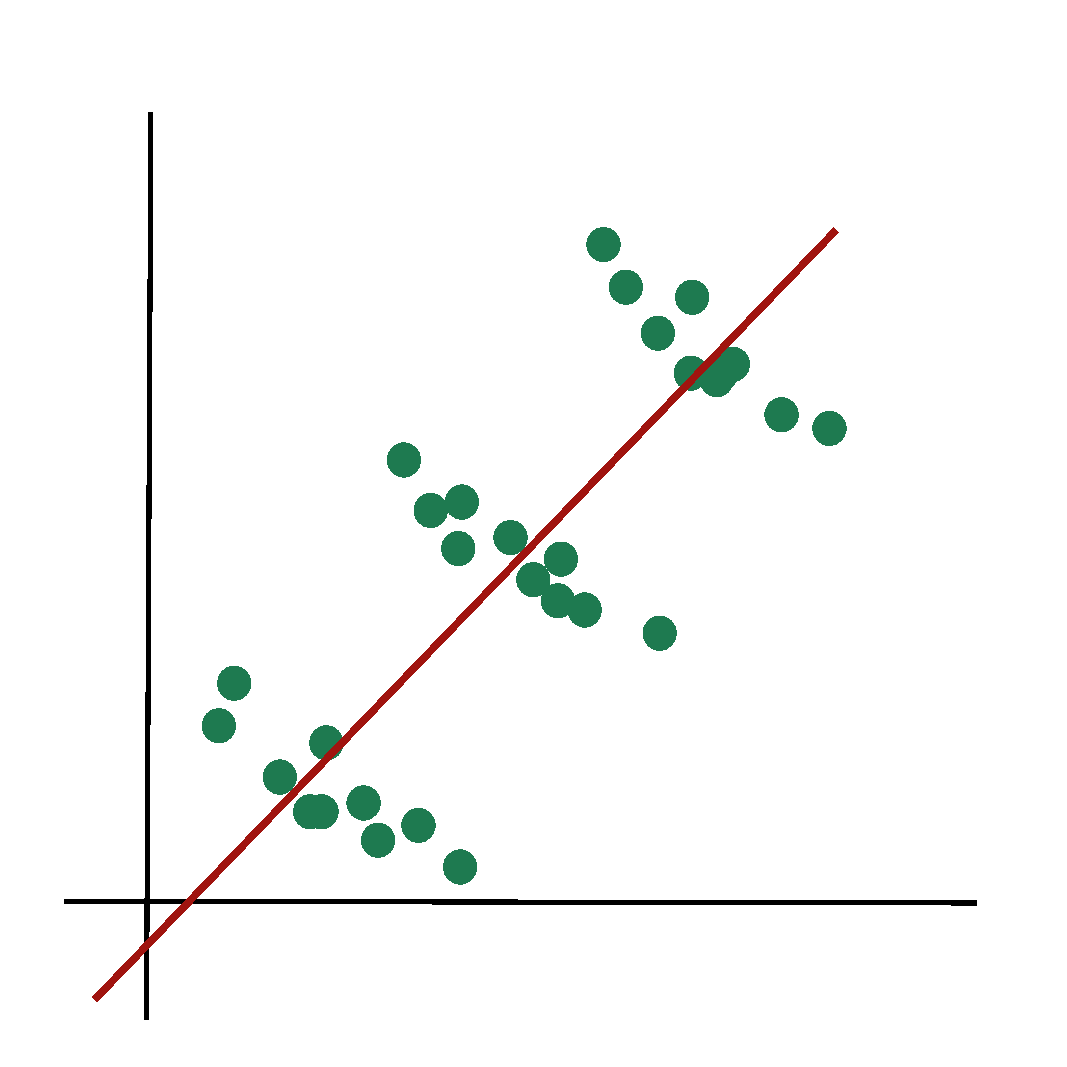
\includegraphics[scale=.2]{pics/simpson}
\end{center}
This together with examples on Slides~\ref{SP} and~\ref{SP2} shows how important is to observe all variables relevant for the causal analysis. \\[.2cm]
Often there is a way to tell that such a missing variable exists.
\end{frame}

\begin{frame}[fragile]{Fixed graph}
	If the graph is fixed then, at least in principle, estimation can be performed using the \alert{EM algorithm} (usual disadvantages).\\[.3cm]
	If the  graph is decomposable, the M-step is given in closed form.\\[.3cm]
	A typical example is the latent class model or the factor analysis model. Several R packages are available. 
%	\begin{lstlisting}
%		library(poLCA)
%	\end{lstlisting}
\end{frame}

\begin{frame}{Learning the graph structure}


Learning the graph structure in the presence of latent variables is hard:
\begin{itemize}
	\item The number of possible graphs is too large (in fact infinite).
	\item Estimation for each fixed graph is relatively complicated.
	\item Models with latent variables fail many regularity assumptions used in standard asymptotic statistics.
\end{itemize}
\begin{alertblock}{Latent tree models}
	Given the data $Y$ finding the maximal likelihood tree is done easily and efficiently (Chow-Liu algorithm).\\[.3cm] 
	The set of trees with leaves $X$ is finite.\\[.3cm] 
\end{alertblock}

\end{frame}

\subsection{Latent tree models}

\begin{frame}[plain,noframenumbering]{}
\begin{center}
	{\huge \textcolor{DarkRed}{4.1 Latent tree models}}
\end{center}
\end{frame}


\begin{frame}{Trees}
\begin{itemize}
\item \textbf{Definition}: \textcolor{blue}{Tree} $=$ undirected graph without cycles\\[.3cm]
\item a tree $T=(V,E)$: $V$ \textcolor{blue}{vertices},\quad $E$ \textcolor{blue}{edges}\\[.4cm]
\begin{minipage}{4cm}
\begin{center}
\tikzstyle{vertex}=[circle,fill=black,minimum size=5pt,inner sep=0pt]
\tikzstyle{hidden}=[circle,draw,minimum size=5pt,inner sep=0pt]
  \begin{tikzpicture}[scale=.7]
  \node[hidden] (1) at (-.7,.7)   {};
    \node[hidden] (2) at (-.7,-.7) {};
    \node[hidden] (3) at (1.1,.9) {};
    \node[hidden] (4) at (2.2,.9) {};
    \node[hidden] (5) at (4,0.7) {};
    \node[hidden] (6) at (4,-.7) {};
    \node[hidden] (a) at (0,0) {};
    \node[hidden] (b) at (1.1,0) {};
    \node[hidden] (c) at (2.2,0) {};
     \node[hidden] (d) at (3.3,0) {};
     \draw[line width=.3mm] (a) to (1);
    \draw[line width=.3mm] (a) to (2);
    \draw[line width=.3mm] (a) to (b);
    \draw[line width=.3mm] (b) to (3);
    \draw[line width=.3mm] (b) to (c);
    \draw[line width=.3mm] (c) to (4);
   \draw[line width=.3mm] (d) to (c);
   \draw[line width=.3mm] (d) to (5);
   \draw[line width=.3mm] (d) to (6);
  \end{tikzpicture}\\
  undirected
  \end{center}
\end{minipage}\hspace{1cm}
\begin{minipage}{4cm}
\begin{center}
\tikzstyle{vertex}=[circle,fill=black,minimum size=5pt,inner sep=0pt]
\tikzstyle{hidden}=[circle,draw,minimum size=5pt,inner sep=0pt]
  \begin{tikzpicture}[scale=.7]
  \node[hidden] (1) at (-.7,.7)   {};
    \node[hidden] (2) at (-.7,-.7) {};
    \node[hidden] (3) at (1.1,.9) {};
    \node[hidden] (4) at (2.2,.9) {};
    \node[hidden] (5) at (4,0.7) {};
    \node[hidden] (6) at (4,-.7) {};
    \node[hidden] (a) at (0,0) [label=above:$r$]{};
    \node[hidden] (b) at (1.1,0) {};
    \node[hidden] (c) at (2.2,0) {};
     \node[hidden] (d) at (3.3,0) {};
     \draw[->,-latex,line width=.3mm] (a) to (1);
    \draw[->,-latex,line width=.3mm] (a) to (2);
    \draw[->,-latex,line width=.3mm] (a) to (b);
    \draw[->,-latex,line width=.3mm] (b) to (3);
    \draw[->,-latex,line width=.3mm] (b) to (c);
    \draw[->,-latex,line width=.3mm] (c) to (4);
   \draw[->,-latex,line width=.3mm] (c) to (d);
   \draw[->,-latex,line width=.3mm] (d) to (5);
   \draw[->,-latex,line width=.3mm] (d) to (6);
  \end{tikzpicture}\\
  \textcolor{blue}{rooted}
  \end{center}
\end{minipage}
\end{itemize}
\vspace{.5cm}
\begin{minipage}{6cm}
\begin{itemize}
\item rooted tree often depicted as\ldots\\[.3cm]
\item \textcolor{blue}{leaves}=degree one nodes\\[.3cm]
\item \textcolor{blue}{inner nodes}=degree $\geq 2$ nodes
\end{itemize}
\end{minipage}
\begin{minipage}{4cm}
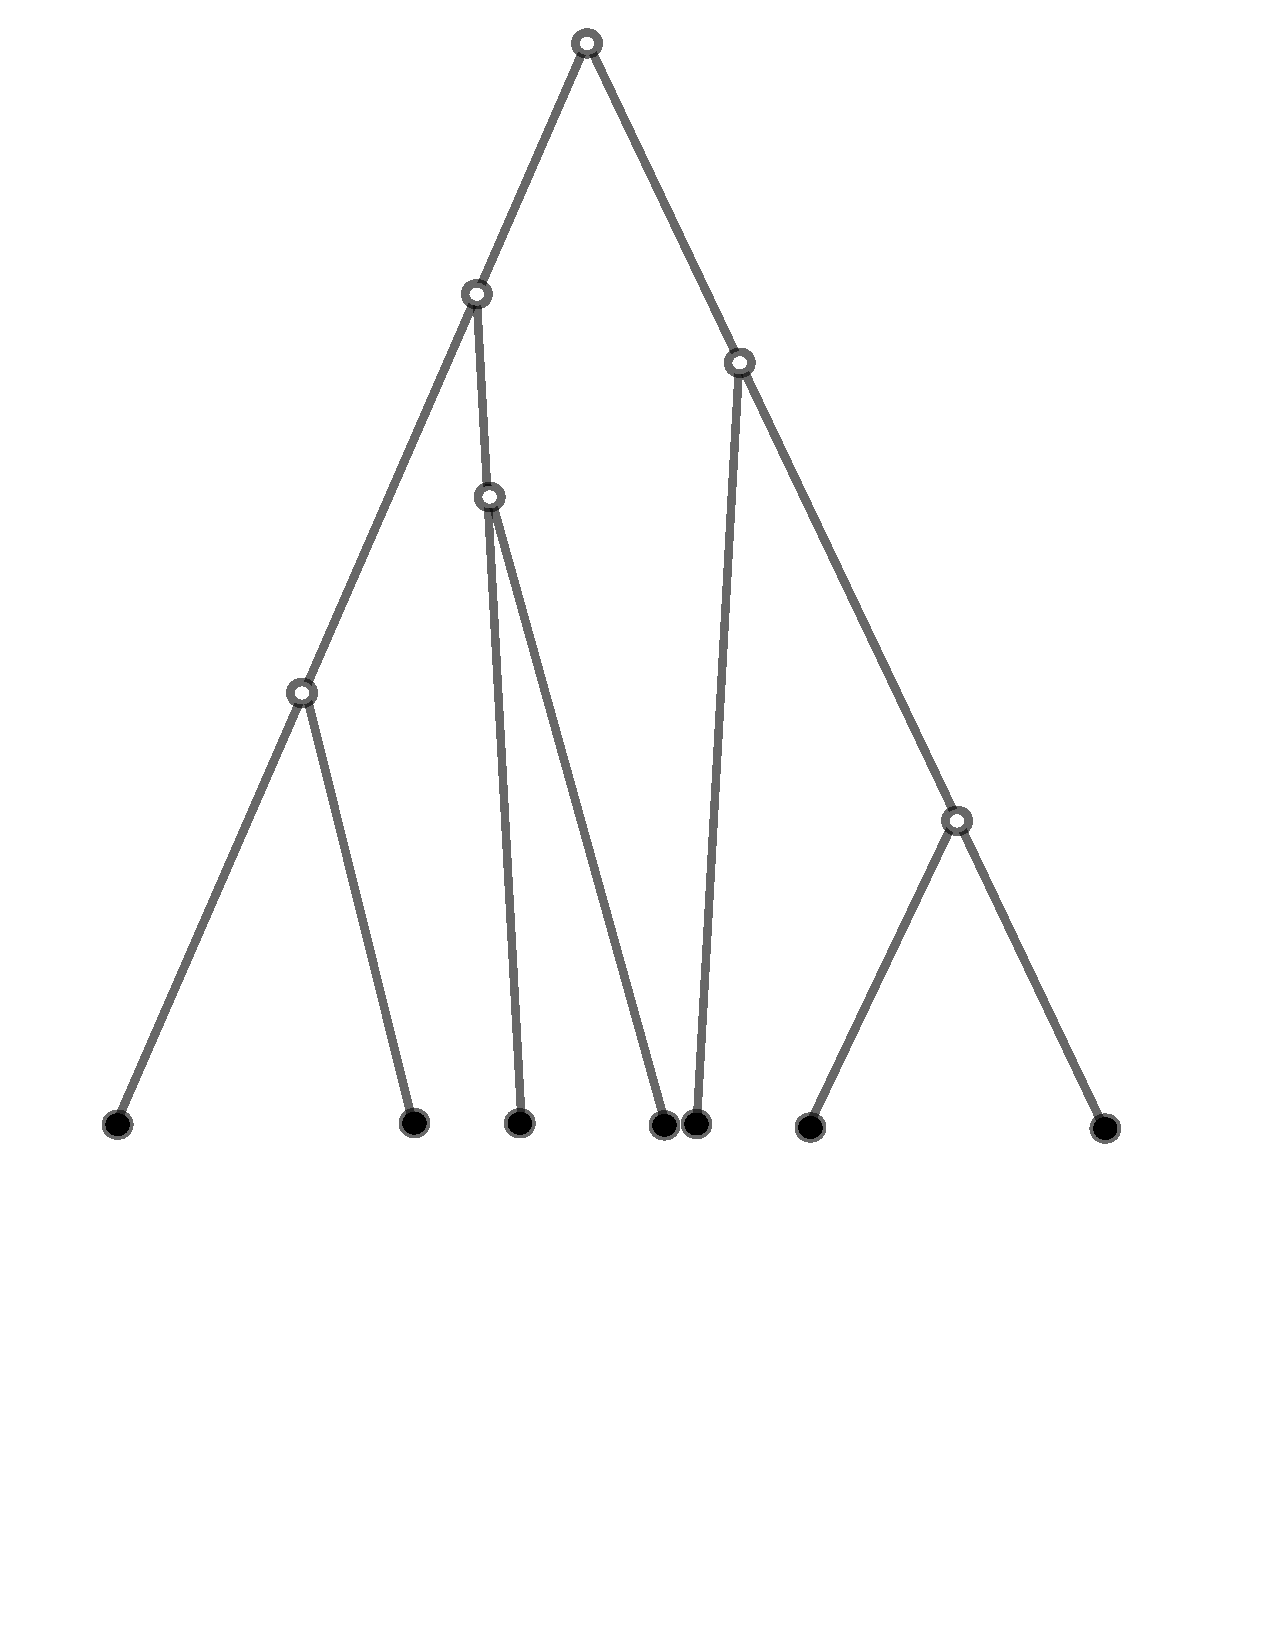
\includegraphics[scale=.15]{./pics/rtree}
\end{minipage}
\end{frame}



\begin{frame}{Latent tree models}
		\begin{alertblock}{One step away from tree models}
\begin{itemize}
\item Graphical models on trees have many nice properties: 
\begin{itemize}
\item exponential families with explicit formulas for the MLE,
\item dynamic programming for efficient computations of various probabilistic quantities.
\end{itemize}
\item Making some of the variables hidden gives greater flexibility.\end{itemize}
	\end{alertblock}
	\begin{alertblock}{Naive definition of latent tree models}
\begin{itemize}
\item \textcolor{blue}{Tree-decomposable distribution} a marginal distribution of a tree distribution.
\item Discussed by J. Pearl as a natural extension of star-decomposable distributions (mixture model, naive Bayes model, latent class model)
\end{itemize}
	\end{alertblock}
	{\tiny Judea Pearl, \textit{Fusion, Propagation, and Structuring in Belief Networks}, Artificial Inteligence, 1986.
	}
\end{frame}


\begin{frame}{Motivation}
	\begin{alertblock}{Statistical motivation}
	\begin{itemize}
	\item Applications in: 
	\begin{itemize}
	\item phylogenetics and linguistics -- to model evolutionary processes,
	\item hierarchical clustering,
	\item image processing and network tomography.
	\end{itemize}
	\item Important concept in causality.
	\item Many well known statistical models are submodels:
	\begin{itemize}
	\item hidden Markov models and naive Bayes models,
	\item phylogenetic models of evolution.
	\end{itemize}
	\end{itemize}
	\end{alertblock}\vspace{-.3cm}
\begin{alertblock}{Mathematical motivation}
\begin{itemize}
\item Understand models with hidden data:
\begin{itemize}
\item identifiability, model constraints, 
\item geometry of the likelihood function.
\end{itemize}
\end{itemize}
\end{alertblock}
	{\tiny 	Alan S. Willsky, \textit{Multiresolution Markov Models for Signal and Image Processing}, 2002.\\
	Martin J. Wainwright, Michael I. Jordan, \textit{Graphical Models, Exponential Families, and Variational Inference}, 2008.\\
	}

\end{frame}



\subsection{High-dimensional Gaussian graphical models}

\begin{frame}[plain,noframenumbering]{}
\begin{center}
	{\huge \textcolor{DarkRed}{4.2 High-dimensional Gaussian graphical models}}
\end{center}
\end{frame}

\begin{frame}{Learning the graph in high-dimensions}
Let $Y=(X,H)$ be a \alert{Gaussian} vector.
\begin{alertblock}{Low-Rank Plus Sparse estimator}
 Then using standard matrix algebra
	$$
	(\Sigma_{XX})^{-1}=K_{XX}-K_{XH}K_{HH}^{-1}K_{HX}.
	$$
	If the underlying graph of $Y$ is sparse then $K$ (and so also $K_{XX}$) is a sparse matrix. \\[.3cm]
	If the length of $H$ is relatively small compared to $X$ then $K_{XH}K_{HH}^{-1}K_{HX}$ has small rank. \\[.3cm]
	In that case $(\Sigma_{XX})^{-1}$ can be written as $S+L$, where $S$ is \textcolor{SeaGreen}{sparse} and $L$ is \textcolor{SeaGreen}{low rank}.
	\end{alertblock}	
\end{frame}

\begin{frame}{}
	Assuming that $(\Sigma_{XX})^{-1}=S+L$ where $S$ is sparse and $L$ has low rank, we can try to recover $S$ and $L$ using convex optimization techniques.  
	$$
	\mbox{maximize} \;\;\;\log\det(S+L)-{\rm tr}(W(S+L))\;+\;\lambda \|S\|_1\;+\;\gamma\|L\|_*,
	$$
where $W$ is the sample covariance matrix, $\lambda, \gamma$ are positive constants, and $\|L\|_*=\sum_i \sigma_i(L)$ denotes the \alert{nuclear} norm of $L$. \\[.2cm]


The nuclear norm is a convex envelope of the rank function restricted to matrices with operator norm $\leq 1$. ({\footnotesize Details in the PhD thesis of Maryam Fazel ``Matrix rank minimization with applications'' (1300 Google citations)})
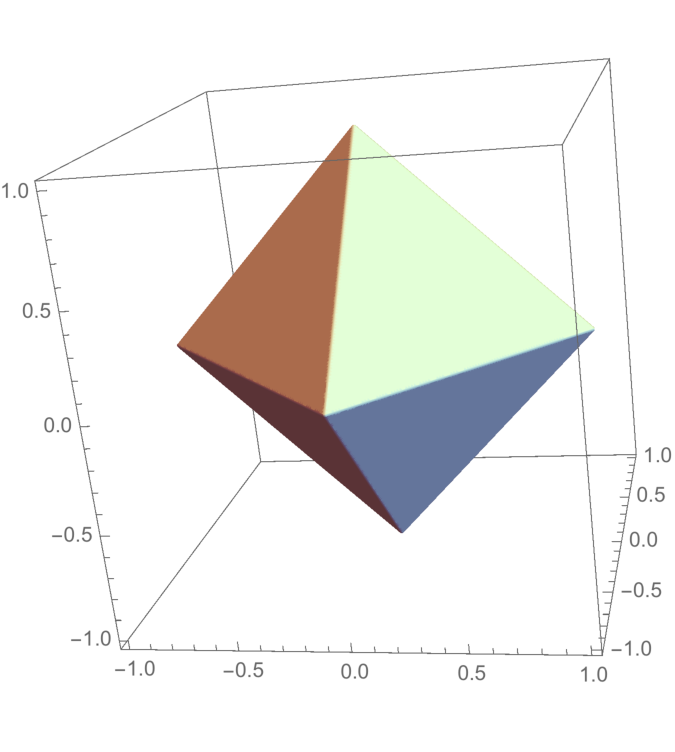
\includegraphics[scale=.3]{pics/lasso_ball}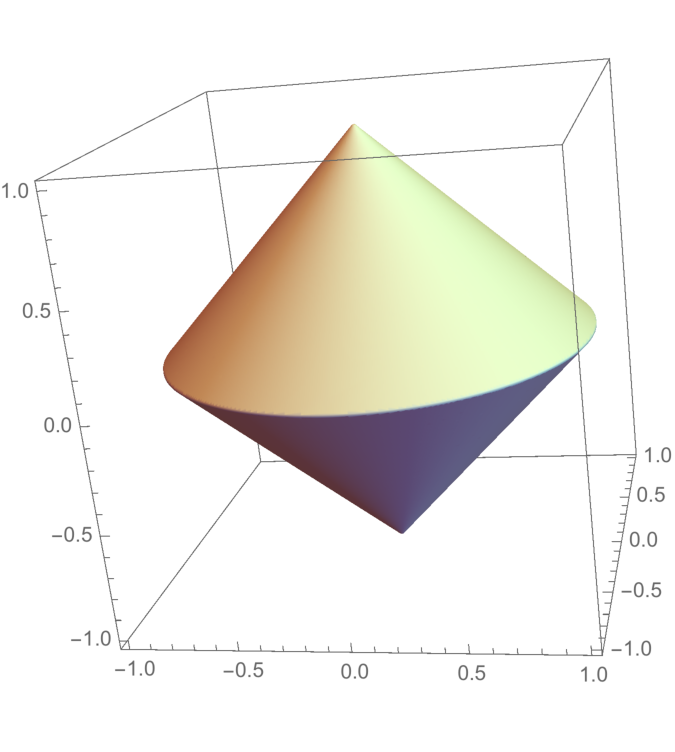
\includegraphics[scale=.3]{pics/glasso_ball}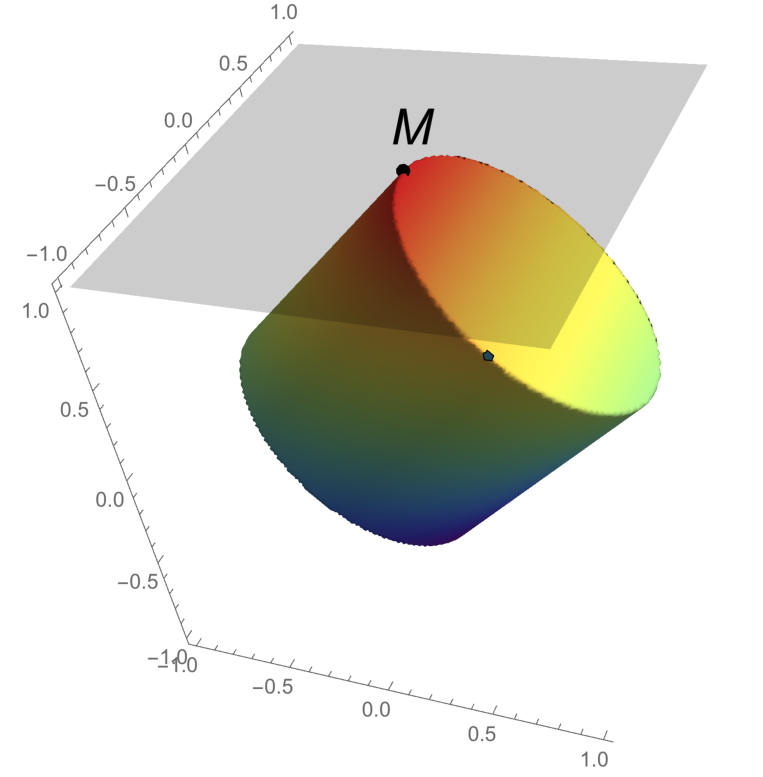
\includegraphics[scale=.25]{pics/nuclear}
\end{frame}

\begin{frame}[fragile]{Using an R implementation}
As an example study the personality traits data on Slide~\ref{pers_lasso}.
	\begin{lstlisting}
install.packages("devtools"); library(devtools)
install_github("benjaminfrot/lrpsadmm")
library(lrpsadmm)
gammas <- c(0.1, 0.15, 0.2)
cvpath <- lrpsadmm.cv(x[,1:80], gammas = gammas,
                         lambda.ratio = 1e-02, n.lambdas = 30, verbose = TRUE)
best.gamma <- cvpath$best.gamma
best.lambda <- cvpath$best.lambda
best.fit <- cvpath$best.fit$fit
Khat <- -cov2cor(solve(best.fit$S)); diag(Khat) <- 1; rownames(Khat) <- colnames(Khat) <- colnames(x[,1:80])
qgraph::qgraph(Khat,layout="spring",threshold=1e-2)
sum(abs(eigen(best.fit$L)$values)>1e-10) # gives that the rank of L is 11.
# to get more information about the stocks
> which(stockdata$info[,1]=="COG")
[1] 70
> stockdata$info[70,]
               V1                V2                V3 
            "COG"          "Energy" "Cabot Oil & Gas" 
	\end{lstlisting}
	Some extensions to generalized linear models are forthcoming.
\end{frame}

\begin{frame}{}
	\begin{center}
		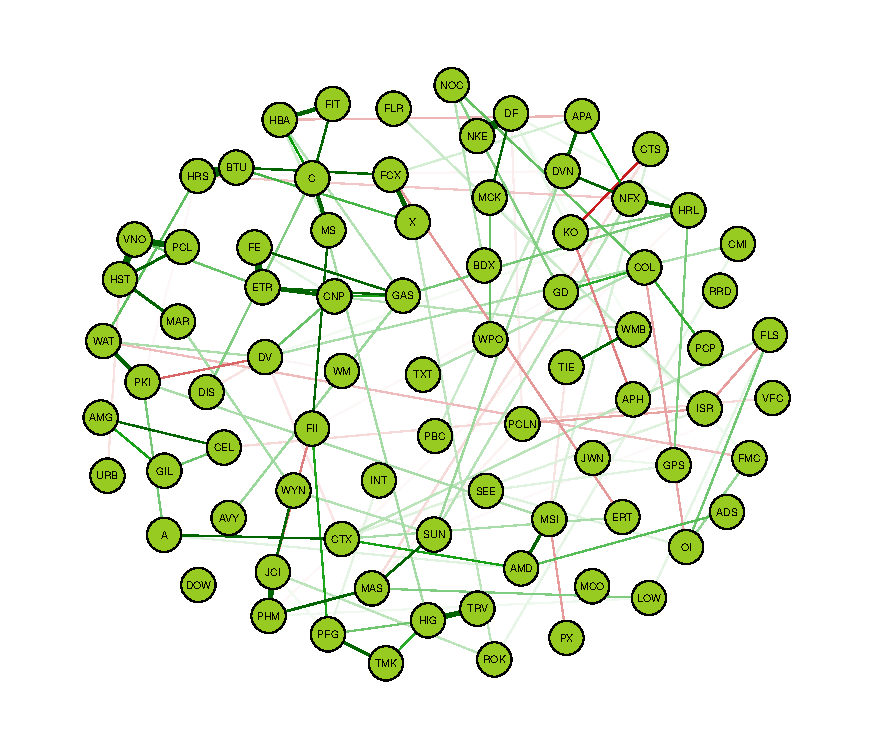
\includegraphics[scale=.9]{pics/stocks_latent}
	\end{center}
\end{frame}

\begin{frame}{}
Thresholding partial correlations $<0.05$ gives a very sparse graph.
	\begin{center}
		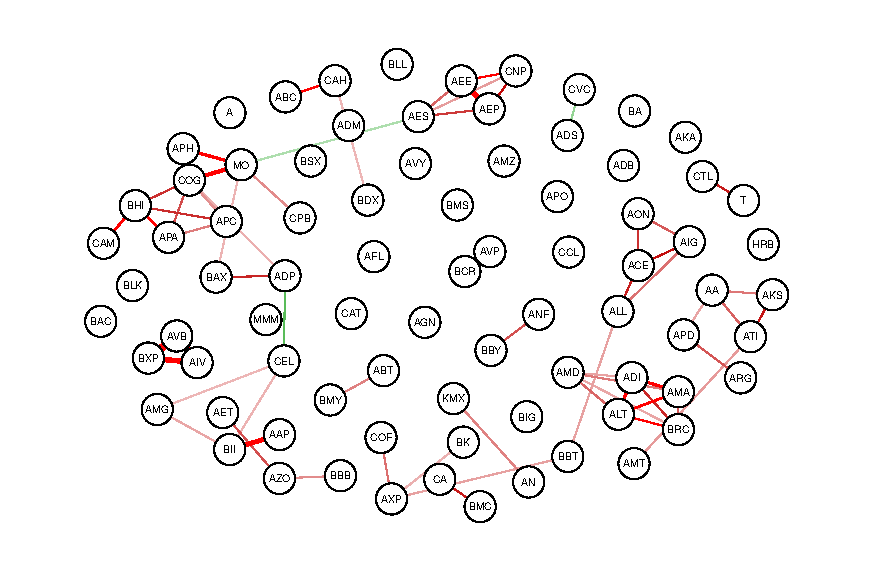
\includegraphics[scale=.9]{pics/stocks_latent2}
	\end{center}
\end{frame}


\begin{frame}{Other interesting models/packages}
\texttt{mgm} - Estimation of k-Order time-varying Mixed Graphical Models and mixed VAR(p) models via elastic-net regularized neighborhood regression.\\[.2cm]
	\texttt{mixggm} - Mixtures of Gaussian graphical models for model-based clustering with sparse covariance and concentration matrices.\\[.2cm]
	\texttt{NetworkChange} - Network changepoint analysis for undirected network data.\\[.2cm]
	\texttt{graphicalVAR} - Estimates within and between time point interactions  using the Graphical VAR model in combination with regularization.\\[.2cm]
	\texttt{mlVAR} - Estimates the multi-level vector autoregression model on time-series data. Three network structures are obtained: temporal networks, contemporaneous networks and between-subjects networks.\\[.2cm]

\texttt{SparseTSCGM} - Computes sparse autoregressive coefficient and precision matrices for time series chain graphical models(TSCGM).\\[.3cm]
	\begin{beamercolorbox}[wd=\paperwidth,sep=5pt]{important}
	Related articles are on our reading list.	
	\end{beamercolorbox}

\end{frame}


%\begin{frame}{Extensions to generalized linear models}
%	Amnir Taeb
%\end{frame}


%\section{Models for temporal data}
%\begin{frame}[plain,noframenumbering]{}
%\begin{center}
%	{\Huge \textcolor{DarkRed}{Part 5: Models for temporal data}}
%\end{center}
%\end{frame}

%\begin{frame}{Package \texttt{mgm}}
%	Estimation of k-Order time-varying Mixed Graphical Models and mixed VAR(p) models via elastic-net regularized neighborhood regression.
%\end{frame}


\section{Positive association}
\begin{frame}[plain,noframenumbering]{}
\begin{center}
	{\Huge \textcolor{DarkRed}{Part 6: Positive association}}
\end{center}
\end{frame}




\begin{frame}[plain,noframenumbering]{}
\begin{center}
	{\huge \textcolor{DarkRed}{6.1 Basic concepts}}
\end{center}
\end{frame}


%\begin{frame}{Notation}
%%\begin{block}{}
%\begin{itemize}
%\item  $X=(X_{1},\ldots,X_{m})$,\quad $V:=\{1,\ldots,m\}$\\[.5cm]
%\item state space: $\cX=\prod_{i\in V} \cX_{i}$
%\begin{itemize}
%\item discrete case $\cX_{i}=\{0,\ldots,r_{i}-1\}$, or
%\item Gaussian case $\cX=\R^{m}$.\\[.5cm]
%\end{itemize}
%\item For $x,y\in \cX$ denote:
%\begin{itemize}
%\item \textcolor{blue}{$x\geq y$} \quad if $x_{i}\geq y_{i}$ for all $i=1,\ldots,m$,
%\item \textcolor{blue}{$x\wedge y$} \;\;=\;\; coordinatewise minimum
%\item \textcolor{blue}{$x\vee y$} \;\;=\;\; coordinatewise maximum
%\end{itemize}
%\end{itemize}
%%\end{block}
%%\begin{alertblock}{}
%%\begin{itemize}
%%\item probability \textcolor{blue}{density} function $p(x)$ on $\cX$
%%%\item in the discrete case $p\in \R^{\cX}=\R^{r_{1}\times \cdots\times r_{m}}$ is a \textcolor{blue}{tensor}
%%\begin{itemize}
%%\item sometimes \,\, \textcolor{blue}{$p_{x}$} \,\,for $p(x)$ if $\cX$ discrete
%%\item the underlying measure is a product measure.
%%\end{itemize}
%%\end{itemize}
%%\end{alertblock}
%\end{frame}


\begin{frame}
\frametitle{Definition}
	\begin{itemize}
\item $X=(X_{1},\ldots,X_{m})$, $\cX=\prod_{i=1}^m\cX_i\subset \R^m$, density $p$.\\[.7cm]
\item A function $p$  is \alert{$\mtp$} if:
$$
p(x)\,p(y)\;\;\leq\;\; p(x\wedge y)\,p(x\vee y)\qquad\mbox{for all }x,y\in \cX.
$$
\vspace{-.5cm}
\begin{itemize}
\item e.g. $p(1,1,0)p(0,0,1)\leq p(0,0,0)p(1,1,1)$\\[.7cm]
 \end{itemize}
% \item $X=(X_{1},\ldots,X_{m})$ is $\mtp$ if its distribution is.\\[.7cm] 
 \item If $p>0$ the condition simplifies.\\[.2cm]
\begin{itemize}
\item e.g. $p(1,1,0)p(0,1,1)\leq p(0,1,0)p(1,1,1)$\\[.7cm]
 \end{itemize}
 \end{itemize}
%\pause
\end{frame}

\begin{frame}{Original motivation}
	\begin{itemize}
\item $X=(X_{1},\ldots,X_{m})$ is \alert{positively associated} if for any two \textit{non-decreasing} functions $\phi,\psi:\R^m\to \R$
$${\rm corr}\{\phi(X),\psi(X)\}\geq 0.$$
\end{itemize}	
\vspace{.5cm}
\begin{alertblock}{Theorem[FKG inequality]}
	\qquad $\mtp$\qquad $\Longrightarrow$\qquad positively associated.	
\end{alertblock}
	\begin{itemize}
\item e.g. ferromagnetic Ising models
\end{itemize}
{\scriptsize Fortuin, Kasteleyn, Ginibre, \textit{Correlation inequalities on some partially ordered sets}, 1971.}

\end{frame}

\begin{frame}
\frametitle{Basic properties}
If $X=(X_{1},\ldots,X_{m})$ is $\mtp$, then\\[.3cm]
\begin{itemize}
\item[(i)] any \textbf{marginal} distribution is $\mtp$;\\[.3cm]
\item[(ii)] any  \textbf{conditional} distribution is $\mtp$,
\end{itemize}
\vspace{.7cm}
{\footnotesize S. Karlin, Y. Rinott, \textit{Classes of orderings of measures and related correlation inequalities. I. Multivariate totally positive distributions}, JMVA, 1980.}
\bigskip

\alert{There is no Yule-Simpson paradox!}
%\pause
%\pause
%\begin{itemize}
%	\item Independence structure for $\mtp$ vector $X=(X_1,\ldots,X_m)$
%\begin{itemize}
%\item $X_{i}\indep X_{j}$ if and only if ${\rm cov}(X_{i},X_{j})=0$.
%\item $X$ can be split into independent blocks and within each block all covariances are \alert{strictly} positive.
%\end{itemize}
%\vspace{.2cm}
%%\pause
%\item Conditional independence structure: for example \alert{upward stability} 
%\begin{itemize}
%\item $X_{A}\indep X_{B}|X_{C}$ implies $X_{A}\indep X_{B}|X_{C\cup \{k\}}$
%\item see also: K. Sadeghi, \textit{Faithfulness of Probability Distributions and Graphs}, JMLR 2017.  
%\end{itemize}
%\end{itemize}
 \end{frame}



%\begin{frame}{Conditional independence structure}
%\begin{block}{}
%In [\alert{\small S. Fallat, et al, Total positivity in Markov structures, AoS,  2017}] we studied Markov structures of $\mtp$ distributions.
%\end{block}
%
%	\begin{itemize}
%	\item Independence structure
%\begin{itemize}
%\item ${\rm cov}(X_{i},X_{j})=0$ implies that $X_{i}$ independent of $X_{j}$.
%\item $X$ can be split into independent blocks and within each block all covariances are \alert{strictly} positive.
%\end{itemize}
%\vspace{.2cm}
%%\pause
%\item Conditional independence structure: for example \alert{upward stability} 
%\begin{itemize}
%\item $X_{A}\indep X_{B}|X_{C}$ implies $X_{A}\indep X_{B}|X_{C\cup \{k\}}$
%\item see also: K. Sadeghi, \textit{Faithfulness of Probability Distributions and Graphs}, JMLR 2017.  
%\end{itemize}
%\end{itemize}
%\end{frame}


%\begin{frame}[plain,noframenumbering]{}
%\begin{center}
%	{\huge \textcolor{DarkRed}{Gaussian $\mtp$}}
%\end{center}
%\end{frame}

\subsection{Elementary examples}

\begin{frame}[plain,noframenumbering]{}
\begin{center}
	{\huge \textcolor{DarkRed}{4.2 Elementary examples}}
\end{center}
\end{frame}


\begin{frame}{Example 1: Three binary variables}
	Example: $X=(X_{1},X_{2},X_{3})\in \{0,1\}^{3}$
		{\small
		\begin{equation*}
\label{eq:super222}
\begin{matrix}
{p_{001} p_{110} \leq p_{000} p_{111}}&& 
{p_{010} p_{101} \leq p_{000} p_{111}}&&
{p_{100} p_{011} \leq p_{000} p_{111}}\\ 
p_{011} p_{101} \leq p_{001} p_{111}&&
p_{011} p_{110} \leq p_{010} p_{111}&&
p_{101} p_{110} \leq p_{100} p_{111} \\
p_{001} p_{010}\leq p_{000} p_{011} &&
p_{001} p_{100}\leq p_{000} p_{101} &&
p_{010} p_{100}\leq p_{000} p_{110} 
\end{matrix}
\end{equation*}}

Note: If $p>0$ then the first row is implied by the other two: 
$$
(p_{011} \alert{p_{101}})(p_{001} \alert{p_{010}})\leq (p_{001} \alert{p_{111}})(\alert{p_{000} }p_{011})
$$
Boundary points satisfy \textcolor{SeaGreen}{context specific independence}:
$$
p_{011} p_{101} = p_{001} p_{111}\qquad\Longleftrightarrow \qquad X_1\indep X_2|\{X_3=1\}
$$
\end{frame}
\begin{frame}{}
\begin{alertblock}{There are various useful reformulations:}
All conditional covariances are nonnegative:
	$$p_{01k} p_{10k} \leq p_{00k} p_{11k}\qquad\Longleftrightarrow\qquad \cov(X_1,X_2|\{X_3=k\})\geq 0.$$
	Equivalently all conditional log-odds ratios are nonnegative:
	$$p_{01k} p_{10k} \leq p_{00k} p_{11k}\qquad\Longleftrightarrow\qquad \log\left(\tfrac{p_{00k} p_{11k}}{p_{01k} p_{10k}}\right)\geq 0.$$	
\end{alertblock}
\begin{beamercolorbox}[wd=\paperwidth,sep=5pt]{important}
Equivalently, $X_1\indep X_2\indep X_3|H$,\;\; $H$ binary, $\cov(X_i,H)\geq 0$.\\	
%{\tiny For details see \cite{LTbook}.}	
\end{beamercolorbox}
%All covariances are nonnegative:
%	$$
%	\cov(X_1,X_1)\;=\;p_{00+}p_{11+}-p_{01+}p_{10+}\;\geq \;0
%	$$
%	(the marginal distribution is $\mtp$)\\[.5cm]
\end{frame}
\begin{frame}{Example 2: Gaussian distribution}
${\rm PD}_{m}=$ symmetric $m\times m$ positive definite matrices \\[.2cm]
{Gaussian distribution} with mean $\mu\in \R^m$ and covariance $\Sigma\in {\rm PD}_{m}$ \\[.2cm]
\alert{concentration matrix} $K:=\Sigma^{-1}$\\[.2cm]
$$p(x;K)\;=\;\tfrac{1}{(2\pi)^{m/2}}(\det K)^{1/2}\exp\{-\tfrac{1}{2}(x-\mu)^TK(x-\mu)\}$$
\bigskip

\begin{beamercolorbox}[wd=\paperwidth,sep=5pt]{important}	
Gaussian $X$ is $\mtp$ if and only if $K_{ij}\leq 0$ for all $i\neq j$.
\begin{itemize}
	\item {\small Equivalently, $K$ is an \textcolor{SeaGreen}{M-matrix} (aka Stieltjes matrix).}
\end{itemize}
 \end{beamercolorbox}
%{\small See \cite{B} and  \cite{karlinGaussian}.}
\end{frame}

\begin{frame}{}
	Recall: The partial correlations satisfy
	$$
	\rho_{ij|V\setminus \{i,j\}}\;=\;-\tfrac{K_{ij}}{\sqrt{K_{ii}K_{jj}}}\;\geq \; 0.
	$$
	\begin{beamercolorbox}[wd=\paperwidth,sep=5pt]{important}	
		For Gaussians partial and conditional correlations are equal.
	\end{beamercolorbox}
	Closure of the $\mtp$ property under marginalization gives:
	$$
	\cov(X_i,X_j|X_{C})\;\geq \;0\qquad \mbox{for every }C\subseteq V\setminus \{i,j\}.
	$$
\smallskip

	\begin{beamercolorbox}[wd=\paperwidth,sep=5pt]{goldbox}	
	The set of M-matrices is \alert{convex} (in $K$). Its boundary is given by some $K_{ij}=0$ (or equivalently $X_i\indep X_j|X_{V\setminus \{i,j\}}$).		
	\end{beamercolorbox}
\end{frame}

\begin{frame}{Binary Ising model}
		The p.m.f. for $x\in \mathcal X=\{-1,1\}^m$ satisfies
$$\log p(x;h,J)\;\;=\;\;h^T x\;+\;\tfrac{1}{2}x^T \!J\,  x\;-\;A(h,J ),	$$
with $h\in \R^m$ and $J\in \R^{m\times m}$ symmetric with zeros on the diagonal.\\[.2cm]
(a log-linear model with only second order interactions)\\[.3cm]
\begin{beamercolorbox}[wd=\paperwidth,sep=7pt]{important}	
Binary Ising model is $\mtp$ if and only if $J_{ij}\geq 0$ for all $i\neq j$. \end{beamercolorbox}

	Similar to the Gaussian case, the hypothesis is convex (in $J$) and:
	$$
	J_{ij}=0\quad\Longleftrightarrow\quad X_i\indep X_j|X_{V\setminus \{i,j\}}.
	$$
\end{frame}


%\begin{frame}{Graphical models}
%	Given a graph $G$ over $V$, the corresponding graphical model $M(G)$ for $X$ is the set of distributions satisfying \textcolor{SeaGreen}{pairwise Markov properties}: if $i$, $j$ not connected by an edge then $X_i\indep X_j|X_{V\setminus \{i,j\}}$.
%	\begin{itemize}
%		\item Gaussian distributions: support of $K=\Sigma^{-1}$.
%		\item Binary Ising models: support of $J$. 
%	\end{itemize}
%\end{frame}
\subsection{Modelling}
\begin{frame}[plain,noframenumbering]{}
\begin{center}
	{\huge \textcolor{DarkRed}{4.3 Modelling}}
\end{center}
\end{frame}


\begin{frame}
\frametitle{A restrictive condition?}
\begin{itemize}
\item $\mtp$ contraints appear to be \textit{restrictive}:
\begin{itemize}
\item  $3$-dim Gaussian: about $5\%$ of distributions are $\mtp$,
\item  $4$-dim Gaussian: about $0{.}09\%$ of distributions are $\mtp$.\\[.4cm]
\end{itemize}
%\item $\mtp$ distributions are \textit{abundant} in real data
\item Less restrictive under additional Markov structure.\\[.4cm]
\item In the $3$-dim case
\begin{itemize}
\item if $1\indep 2|3$  then $25\%$ are $\mtp$
\item if, in addition, $1\indep 3|2$ then $50\%$ are $\mtp$
\item if $1\indep 2\indep 3$  then everything is $\mtp$\\[.4cm]
\end{itemize}
\end{itemize}
Informally: In sparse structures $\mtp$ is more likely.\\[.1cm]
%{\tiny(*)}{\TINY It is more likely to see $\mtp$ distribution in sparse structures especially in settings where total positivity is expected. }
\end{frame}

\begin{frame}
\frametitle{Example 1: EPH-gestosis}
{\footnotesize \begin{itemize}
	\item Dataset collected 45 years ago in a study on ``Pregnancy and Child Development'' %by the German Research Foundation  
\item {EPH-gestosis (pre-eclampsia):} disease \textbf{syndrome} for pregnant women; three \textbf{symptoms} (high body water retention, high amounts of urinary proteins, elevated blood pressure)
%\begin{itemize}
%\item edema (high body water retention)
%\item proteinuria (high amounts of urinary proteins) 
%\item hypertension (elevated blood pressure)
%\end{itemize}	
\item A {syndrome} is a set of medical signs and symptoms that are {correlated} with each other and, often, with a particular disease or disorder. 
%The word derives from the Greek and means \textbf{"concurrence"}. (Wikipedia)
\end{itemize}	}

\begin{beamercolorbox}[wd=\paperwidth,sep=5pt]{result}
	%	\begin{itemize}
%		\item Observed counts:
%\vspace{-.2cm}
{\footnotesize The sample distribution$$
\left[\begin{array}{cccc}
\hat p_{000} & \hat p_{010} & \hat p_{001} & \hat p_{011} \\
\hat p_{100} & \hat p_{110} & \hat p_{101} & \hat p_{111} 
\end{array}\right]= \tfrac{1}{4649}\left[\begin{array}{cccc}
3299 & 107 & 1012 & 58 \\
78 & 11 & 65 & 19
\end{array}\right]
$$
is already $\mtp$. \underline{Equivalently}, $X_1\indep X_2\indep X_3|H$ for a latent binary $H$.}
\end{beamercolorbox}
%\item This sample distribution is $\mtp$.
%\begin{itemize}
%\item \alert{equivalently}: $X_1\indep X_2\indep X_3|H$ for some binary $H$
%	\end{itemize}
%	\end{itemize}
\end{frame}

\begin{frame}{Example 2: Financial time series.}
	Monthly correlations of global stock markets
	{\footnotesize$$
S = \bordermatrix{~ & Nasdaq & Canada & Europe & UK &Australia \cr
              Nasdaq &    1.000 & 0.606 & 0.731 & 0.618 &0.613\cr
              Canada &    0.606 & 1.000 & 0.550 & 0.661 &0.598\cr
              Europe &    0.731 & 0.550 & 1.000 & 0.644 &0.569\cr
              UK &        0.618 & 0.661 & 0.644 & 1.000 &0.615\cr
              Australia & 0.613 & 0.598 & 0.569 & 0.615 &1.000\cr
              }
$$}
{\footnotesize$$
S^{-1} = \bordermatrix{~ & Nasdaq & Canada & Europe & UK &Australia \cr
              Nasdaq &    2.629 & -0.480 & -1.249 & -0.202 &-0.490\cr
              Canada &    -0.480 & 2.109 & -0.039 & -0.790 &-0.459\cr
              Europe &    -1.249 & -0.039 & 2.491 & -0.675 &-0.213\cr
              UK &        -0.202 & -0.790 & -0.675 & 2.378 &-0.482\cr
              Australia & -0.490 & -0.459 & -0.213 & -0.482 &1.992\cr
              }
$$}
Sampled uniformly this happens with prob. $<10^{-6}$!
\end{frame}

\begin{frame}{Example 3: Math grades}
Data:  grades of 88 students in
\texttt{Mechanics, Vectors, Algebra, Analysis, Statistics}
%\vspace{-.2cm}
%\begin{scriptsize}
{\footnotesize$$
S = \bordermatrix{~ & mechanics & vectors & algebra & analysis & statistics \cr
              mechanics &    305.7680 & 127.2226 &101.5794 & 106.2727  & 117.4049\cr
              vectors &    127.2226 & 172.8422 & 85.1573  & 94.6729   & 99.0120\cr
              algebra &    101.5794  & 85.1573 & 112.8860 & 112.1134  & 121.8706\cr
              analysis &        106.2727&  94.6729& 112.1134& 220.3804&  155.5355\cr
              statistics & 117.4049&  99.0120 & 121.8706& 155.5355&  297.7554 \cr
              }
$$}
{\footnotesize$$
S^{-1} = \bordermatrix{~ & mechanics & vectors & algebra & analysis & statistics \cr
              mechanics &    5.2446& -2.4351& -2.7395&  \textcolor{Important}{0.0116}& -0.1430\cr
              vectors &    -2.4351 & 10.4268 &-4.7078 &-0.7928 & -0.1660\cr
              algebra &    -2.7395 &-4.7078 & 26.9548 &-7.0486 &-4.7050\cr
              analysis &        \textcolor{Important}{0.0116} &-0.7928 &-7.0486&  9.8829& -2.0184 \cr
              statistics & -0.1430 & -0.1660 & -4.7050 &-2.0184 & 6.4501\cr
              }
$$}
\end{frame}


\begin{framefont}{\scriptsize}
\begin{frame}{$\mtp$ constraints are often explicit}
\vspace{-.5cm}\begin{center}
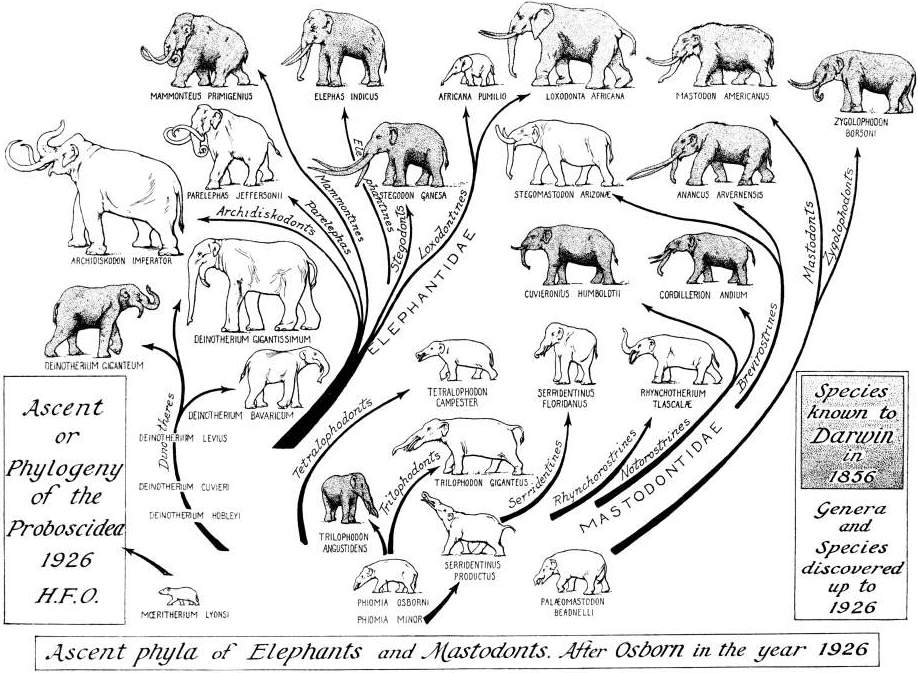
\includegraphics[scale=.25]{pics/phylo_elephants}	
\end{center}\vspace{-.3cm}
	\begin{minipage}{6cm}
		$X$ is $\mtp$ in:
		\begin{itemize}
			\item ferromagnetic Ising models
			\item Markov chains with $\mtp$ transitions
			\item order statistics of \emph{iid} variables
			\item Brownian motion tree model
		\end{itemize}
	\end{minipage}\begin{minipage}{6cm}
		$|X|$ is $\mtp$ in:
		\begin{itemize}
			\item Gaussian/binary tree models
			\item Gaussian/binary latent tree models
			\begin{itemize}
			\item binary latent class models
			\item single factor analysis models
			\end{itemize}
		\end{itemize}
	\end{minipage}
\end{frame}
\end{framefont}

%
%
%\begin{frame}
%\frametitle{Signed $\mtp$ distributions}
%\begin{itemize}
%\item Definition: A Gaussian r.v. $X=(X_1,\ldots,X_m)$ has a \alert{signed $\mtp$} distribution if there exists a diagonal matrix $D\in \{-1,+1\}^m$ such that $DX$ has an $\mtp$ distribution.
%\end{itemize}
%\begin{alertblock}{Theorem (LUZ 2016):}
%	\begin{itemize}
%	\item  Every Gaussian \alert{model on a tree} is signed $\mtp$.
%	\item Signed $\mtp$ property is preserved under taking margins.
%	\begin{itemize}
%		\item single factor analysis models, Gaussian latent tree models, binary latent class models, and binary latent tree models 
%	\end{itemize}
%	\end{itemize}
%	\end{alertblock}
%	\pause
%	\begin{block}{}
%	\begin{itemize}
%		\item Most of the results that I am going to present directly extend from $\mtp$ to signed $\mtp$ distributions.
%	\end{itemize}
%	\end{block}
%\end{frame}
%
%




%\begin{frame}
%\frametitle{Exponential family}
%\begin{itemize}
%\item  
%$p(x;\theta)=g(x)\exp(\langle \theta,T(x)\rangle -A(\theta))$, \quad $\theta\in C\subseteq \R^{d}$, $x\in \cX$.
%\begin{itemize}
%\item (sufficient statistics) $T:\,\cX\to \R^{d}$
%\item (\alert{canonical parameters}) $C=\{\theta:\, \int \exp(\langle \theta,T(x)\rangle)\nu({\rm d}x)<\infty\}$
%\end{itemize}
%\item $C$ is convex and $A(\theta)$ is strictly convex in $C$
%\end{itemize}
%\pause 
%\begin{itemize}
%\item $x^{(1)},\ldots,x^{(n)}\in \cX$ independent sample;\quad $\bar T:=\tfrac{1}{n} \sum_i T(x^{(i)})$
%\item the log-likelihood function:\quad $\ell(\theta)=n\langle \theta,\bar T\rangle -nA(\theta)$
%\item $\ell$ strictly concave in $C$ and so the MLE is unique (if exists) 
%\end{itemize}
%\pause
%\begin{itemize}
%\item \textbf{Theorem (LUZ)}:  The set of all $\theta\in C$ such that $p(x;\theta)$ is $\mtp$ is an intersection of $C$ with a closed \textcolor{Important}{convex} set $\Gamma$. For graphical models $\Gamma$ is a \alert{non-empty polyhedral}    cone.
%\begin{itemize}
%\item the MLE is unique
%\item the boundary decomposes into smaller $\mtp$ exponential families
%\end{itemize}
%\end{itemize}
%\end{frame}

%\begin{frame}
%\frametitle{The maximum likelihood estimator}
%%\begin{itemize}
%\item  $p(x)=g(x)\exp(\langle \theta,T(x)\rangle -A(\theta))$, $\theta\in C\subseteq \R^{d}$, $x\in \cX$.
%\end{itemize}
%%%\begin{itemize}
%\item $x^{(1)},\ldots,x^{(n)}\in \cX$ independent data;\quad $\bar T:=\tfrac{1}{n} T(x^{(i)})$
%\item the log-likelihood function:\quad $\ell(\theta)=n\langle \theta,\bar T\rangle -nA(\theta)$
%\item $\ell$ strictly concave in $C$ and so the MLE is unique (if exists) 
%\end{itemize}
%%%\begin{itemize}
%\item MLE exists \quad if and only if \quad$\bar T\in {\rm int}(K)$.
%\item It is given by the unique point in the preimage of $-\nabla A(\theta)$.
%\end{itemize}
%%\end{frame}

%\begin{frame}
%\frametitle{$\mtp$ exponential family}
%%\begin{itemize}
%\item Describe all $\theta\in C$ such that $p(x;\theta)$ is $\mtp$.
%\item \textbf{Proposition}: It is an intersection of $C$ with a relatively closed convex set $\Gamma$.
%\begin{itemize}
%\item Remark: Typically $\Gamma$ is a cone. 
%\end{itemize}
%\end{itemize}
%%%Proof sketch:
%\begin{itemize}
%\item check $\Delta(x,y;\theta)=\log\left(\tfrac{p(x\wedge y;\theta)p(x\vee y;\theta)}{p(x;\theta)p(y;\theta)}\right)\geq 0$ for all $x,y$
%\item $\Delta(x,y;\theta)$ is linear in $\theta$
%\end{itemize}
%%%\begin{itemize}
%\item \textbf{Theorem}: For graphical models $\Gamma$ is non-empty and polyhedral.
%\end{itemize}
%%{\tiny joint work with Steffen Lauritzen and Caroline Uhler; soon to be on arXiv}
%\end{frame}
%
%\begin{frame}
%\frametitle{Quadratic families}
%%\begin{itemize}
%\item $p(x)=\exp(-\sum_{i,j=1}^{m}\theta_{ij}x_{i}x_{j}-A(\theta))$
%\end{itemize}
%%%\begin{itemize}
%\item Proposition: A quadratic exponential family is $\mtp$ if and only if $\theta_{ij}\leq 0$ for all $i\neq j$.
%\item The parameter space is the negative orthant.
%\item The boundary corresponds to some sparse submodels.
%\end{itemize}
%%%\begin{itemize}
%\item Theorem: The maximum likelihood exists as long as the sample size $\geq 2$. In particular, the MLE estimator makes sense also in the high dimensional setting. 
%\end{itemize}
%%\end{frame}
%
%



%\begin{frame}
%\frametitle{Example: Gaussian $\mtp$ distributions}
%%\begin{itemize}
%\item ${\rm PD}_{m}=$ symmetric $m\times m$ positive definite matrices 
%\item $m$-dimensional \alert{Gaussian distribution} with covariance $\Sigma\in {\rm PD}_{m}$ 
%\item concentration matrix $K:=\Sigma^{-1}$
%\item Gaussian $X$ is $\mtp$ if and only if $K_{ij}\leq 0$ for all $i\neq j$
%\end{itemize}
%%%\begin{itemize}
%\item \textit{i.i.d.} data: $x^{(1)},\ldots,x^{(n)}\in \R^{m}$
%\item sample covariance matrix: $S=\tfrac{1}{n}\sum_{i} x^{(i)}(x^{(i)})^{T}$
%\item the \alert{log-likelihood function}: $\ell(K)=\log\det K-{\rm tr}(SK)$
%\end{itemize}
%%\end{frame}

%\begin{frame}[plain,noframenumbering]{}
%\begin{center}
%	{\huge \textcolor{DarkRed}{Sparse structures}}
%\end{center}
%\end{frame}

\begin{frame}{Recall: Two special cases}
\begin{beamercolorbox}[wd=\paperwidth,sep=5pt]{result}
	\alert{Gaussian model}: $f(x)\;=\;\tfrac{1}{(2\pi)^{p/2}}\sqrt{\det K}\exp(-x^T\!K\,x/2)$\\[.2cm]
$\mtp$ \quad$\Longleftrightarrow$\quad $K=\Sigma^{-1}$ satisfies $K_{ij}\leq 0$ for all $i\neq j$.
%\medskip
%\begin{itemize}
%	\item $K_{ij}\leq 0$ if and only if ${\rm corr}(X_i,X_j|X_{V\setminus \{i,j\}})\geq 0$.\\[.3cm]
%	\item ${\rm corr}(X_i,X_j|X_{A})\geq 0$ for every $A\subseteq V\setminus \{i,j\}$.
%\end{itemize}	
\end{beamercolorbox}
\medskip
\begin{beamercolorbox}[wd=\paperwidth,sep=5pt]{result}
	\alert{Binary Ising model}: $f(x)\;=\;\tfrac{1}{Z(h,J)}\exp(h^Tx+x^T\!J\,x/2)$\\[.2cm]
$\mtp$ \quad$\Longleftrightarrow$\quad $J_{ij}\geq 0$ for all $i\neq j$.
%\medskip
%\begin{itemize}
%	\item $K_{ij}\leq 0$ if and only if ${\rm corr}(X_i,X_j|X_{V\setminus \{i,j\}})\geq 0$.\\[.3cm]
%	\item ${\rm corr}(X_i,X_j|X_{A})\geq 0$ for every $A\subseteq V\setminus \{i,j\}$.
%\end{itemize}	
\end{beamercolorbox}

\bigskip
Convex constraint on the space of the (canonical) parameters with the boundary given by zeros. \\[.3cm]
Informally: In estimation $\mtp$ leads to sparsity.
\end{frame}


\begin{frame}[plain,noframenumbering]{}
\begin{center}
	{\huge \textcolor{DarkRed}{4.2 Gaussian models and finance}}
\end{center}
\end{frame}



\begin{frame}
\frametitle{MLE for Gaussian models}
\begin{itemize}
\item ${\rm maximize}\{\log\det K-{\rm tr}(SK)\}$ over $K\in \mtp$.\\[.5cm]
%\item Dual:  maximize \alert{$\log\det \Sigma$} subject to:
%\begin{itemize}
%\item $\Sigma_{vv}=S_{vv}$ for all $v\in V$
%\item $\Sigma_{uv}\geq S_{uv}$ for all $u\neq v$
%\item $\Sigma\in {\rm PD}_m$
%\end{itemize}
\item The MLE exists iff there exists $\,\Sigma\in {\rm PD}_m$ with $\Sigma\geq S$. \\[.5cm]
\item It is the unique element $\,\hat K = \hat{\Sigma}^{-1}\in {\rm PD}_m$ that satisfies
\begin{itemize}
\item \alert{Primal feasibility:} \;$\hat K_{ij}\leq0\;\; \forall i\neq j,$
\item \alert{Dual feasibility:} \quad $\hat\Sigma_{ii}=S_{ii}\;\; \forall i, \quad \hat\Sigma_{ij}\geq S_{ij}\;\; \forall i\neq j$
%\item[(c)] \alert{Stationarity of Lagrangian:} \, $\tr(S\hat\theta)= m$,
\item \alert{Complimentary slackness:} \;\; $(\hat\Sigma_{ij}-S_{ij}) \,\hat K_{ij}= 0 \;\; \forall i\neq j$.
\end{itemize}
\end{itemize}
\begin{block}{}
	Note: \,\,\, We get zeros in $\hat K$ for free.
\end{block}
\end{frame}


%\begin{frame}{Single-linkage matrix}
%Let $S$ be the sample \emph{correlation} matrix. Assume $S_{ij}\geq 0$ for all $i\neq j$. \\[.5cm]
%	Given the weighted graph of $S$, the single-linkage matrix $Z$ is
%	$$
%	Z_{ij}\;=\;\max_{P\in \mathcal P(i,j)}\min_{uv\in P} S_{uv}\qquad\mbox{for }i\neq j.
%	$$
%	\vspace{-.6cm}
%	\begin{block}{}
%	$\bullet$\;\;	$Z$ is both primarly and dually feasible.
%	\end{block}
%	The fact that $Z\geq S$ (dual feasibility) is easy to establish.\\[.5cm]
%	The fact that $Z^{-1}$ is an M-matrix (primal feasibility) uses the connection to ultrametric matrices:
%	\begin{itemize}
%		\item Proposition: If $S_{ij}<1$ for all $i\neq j$, then $Z$ is non-singular and $Z^{-1}$ is an M-matrix.
%		\item see also: Dellacherie, Martinez, San Martin, \textit{Inverse M-matrices and ultrametric matrices}, Springer,  2014.
%	\end{itemize} 
%\end{frame}
%
%\begin{frame}{Example}
%	Suppose that 
%	$$
%	S\;=\;\begin{bmatrix}
%		1 &-0.5 &0.5 &0.6 \\
%		 -0.5&1 &0.4 &-0.1 \\
%		 0.5& 0.4& 1& 0.2\\
%		 0.6&-0.1 & 0.2&1 		
%	\end{bmatrix}
%	$$
%	Then $Z$ is given by	
%
%\qquad\qquad\begin{minipage}{0.4\textwidth}
%\begin{tikzpicture}[auto, node distance=2cm, every loop/.style={},
%                    main node/.style={circle,draw,font=\large}]
%
%  \node[main node] (1) {1};
%  \node[main node] (2) [below left of=1] {2};
%  \node[main node] (3) [below right of=2] {3};
%  \node[main node] (4) [below right of=1] {4};
%
%  \path[every node/.style={}]
%    (1) edge node [right] {0.6} (4)
%        edge [right] node[left] {0.5} (3)
%    (2) edge [right] node[left] {0.4} (3)
%    (3) edge [right] node[right] {0.2} (4);
%\end{tikzpicture}
%\end{minipage} 
%\begin{minipage}{0.3\textwidth}
%$$
%	Z\;=\;\begin{bmatrix}
%		1 &0.4 &0.5 &0.6 \\
%		 0.4&1 &0.4 &0.4 \\
%		 0.5& 0.4& 1& 0.5\\
%		 0.6&0.4 & 0.5&1 		
%	\end{bmatrix}.
%	$$
%\end{minipage}
%\smallskip
%
%%\begin{beamercolorbox}[wd=\paperwidth,sep=9pt]{notabene}	
%%The maximum cost spanning tree of $S$ plays an important role here. 
%%\end{beamercolorbox}
%\end{frame}


%\begin{frame}
%\frametitle{Example: Carcass data}
%\begin{itemize}
%\item data: thickness of meat and fat layers at different locations on the back of a slaughter pig on each of 344 carcasses 
%\end{itemize}
%$$
%S=\begin{blockarray}{ccccccc}
%\textrm{Fat11} & \textrm{Meat11} & \textrm{Fat12} & \textrm{Meat12} & \textrm{Fat13}&\textrm{Meat13} \\
%\begin{block}{(rrrrrr)l}
%1 & 0.04 & \colorbox{blue!20!white}{0.84} & 0.08 & 0.82 & \textcolor{Important}{-0.03}&\textrm{Fat11}\\ 
%\cdot & 1 & 0.04 & \colorbox{blue!20!white}{0.87} & \colorbox{blue!20!white}{0.13} & 0.86& \textrm{Meat11} \\
%\cdot& \cdot & 1 & 0.01 & \colorbox{blue!20!white}{0.83} & \textcolor{Important}{-0.03}&\textrm{Fat12}\\
%\cdot & \cdot & \cdot & 1 & 0.11 & \colorbox{blue!20!white}{0.90}& \textrm{Meat12} \\
%\cdot & \cdot & \cdot & \cdot & 1& 0.02&\textrm{Fat13} \\
%\cdot & \cdot & \cdot & \cdot & \cdot & 1&\textrm{Meat13} \\
%\end{block}
%\end{blockarray}
%$$
%\begin{itemize}
%	\item Spanning tree: Fat11---Fat12---Fat13---Meat11---Meat12---Meat13
%\end{itemize}
%\end{frame}
%
%
%\begin{frame}
%\frametitle{Example: Carcass data (2)}
%\begin{center}
%\includegraphics[width=4.2cm]{Carcass_MTP2_graph2.pdf}
%\begin{center}
%$\mtp$ constraint
%\end{center}
%\end{center}
%\begin{itemize}
%	\item Only one non-edge satisfies $S_{ij}\geq \prod_{uv\in \overline{ij}}S_{uv}$.
%\end{itemize}
%\end{frame}

\begin{frame}
\frametitle{Existence of the MLE}
Learning sparse structures in high dimensions was the main motivation of {\scriptsize [\alert{Slawski, Hein, \textit{Estimation of positive definite M-matrices and structure learning for attractive Gaussian Markov random fields}, 2015}]}.	\\[.5cm]

\textbf{Theorem (Slawski,Hein(2015))}: The MLE exists with \textit{probability one} for sample size $n\geq 2$.\\[.2cm]
{\small  our proof gives an explicit point that is both primal and dual feasible, it  establishes links to single-linkage clustering, and ultrametrics.}\\[.3cm]
\begin{itemize}
\item Similar results for binary distributions.
\item We provide IPS-type algorithms to fit the model.
\end{itemize}
\end{frame}


\begin{frame}{Fitting the model}
	Give the code
\end{frame}

\begin{frame}{Optimal Markowitz Portfolio}
	Global minimum variance portfolio:\\[.2cm] 
	\hspace{1cm}minimize $w^T\Sigma_t^*w$ subject to $w^T\bs 1=1$.\\[.2cm]
	Replacing the unknown true covariance matrix of returns $\Sigma^*_t$ by some estimator $\hat\Sigma_t$  yields the following analytical solution
	$$
	\hat w\;=\;\tfrac{\hat\Sigma_t\bs 1}{\bs 1^T\hat\Sigma_t\bs 1}
	$$
	In this setting, estimating $\Sigma^*_t$ becomes the main problem.
\end{frame}

\begin{frame}{Covariance matrix estimators}
	Sample covariance is typically a bad estimator of $\Sigma^*_t$.\\[.2cm] 
	Structural assumptions give lower variance (higher bias). 
	\begin{itemize}
		\item Dynamic factor models: Returns for day $t$ are given by a linear combination of a (small) collection of latent factors. \\[.3cm]
		\item Static factor models: As above but $\Sigma_t$ does not depend on $t$. \\[.3cm]
		\item Shrinkage of eigenvalues.\\[.3cm]
		\item Regularization of the precision matrix: graphical lasso, CLIME.
	\end{itemize}
	\end{frame}
	
	\begin{frame}{Exploiting total positivity}
		$\mtp$ constraint gives a natural regularizer.\\[.3cm]
				
		Particularly so when applied to finance:
		\begin{itemize}
			\item \alert{capital asset pricing model (CAPM)} (one factor model with positive loadings) is $\mtp$.  
			\item latent tree models used for unsupervised learning tasks (e.g. clustering similar stocks).
		\end{itemize}
	\bigskip
	
	Data analysis suggests that $\mtp$ regularization performs well where CAPM underfits. It outperforms other methods.
			\end{frame}

\begin{frame}{Extensions to heavy-tailed distributions}
Typically the stocks data  are log-transformed.\\[.4cm]
The log-transformed data may still	be heavy-tailed.\\[.4cm]
With small modifications, similar approach works for elliptical distributions, or more generally, for for \alert{trans-elliptical distributions}.

\begin{beamercolorbox}[wd=\paperwidth,sep=5pt]{goldbox}
	\textbf{Theorem: } If $X$ is $\mtp$ and transelliptical (so that $f(X)$ is elliptical) then $\Sigma^{-1}_f$ is an M-matrix.	
	\end{beamercolorbox}
	The other direction not true, e.g. \alert{no} t-distribution is $\mtp$.
		\begin{beamercolorbox}[wd=\paperwidth,sep=5pt]{important}
		Assuming $\Sigma^{-1}_f$ is an M-matrix we relax the $\mtp$ assumption.
	\end{beamercolorbox}
	\medskip

\end{frame}


%\begin{frame}{Sparsistency}
%Does such a procedure lead to a consistent estimation of the underlying graph? \alert{Of course not.}\\[.3cm]
%
%%For example if the true graph has no edges, the estimated graph will typically not be even very sparse. \\[.3cm]
%
%	Some regularization is needed, see also:
%	{\small
%	\begin{itemize}
%		\item Slawski, Hein, \textit{Estimation of positive definite M-matrices and structure learning for attractive Gaussian Markov random fields}, LAA, 2015. 
%		\item Egilmez, Pavez, Ortega, \textit{Graph Learning from Data under
%Structural and Laplacian Constraints}, 2017.
%%\item Egilmez, Pavez, Ortega, \textit{Learning Graphs with Monotone Topology
%%Properties and Multiple Connected Components}, 2018.\\[.5cm]
%	\end{itemize} }
%	\vspace{-.5cm}
%	\begin{block}{}
%		\textbf{Proposition}: M-matrices are closed under thresholding.
%	\end{block}
%\end{frame}



%\begin{frame}[plain,noframenumbering]{}
%\begin{center}
%	{\huge \textcolor{DarkRed}{Ferromagnetic Ising model}}
%\end{center}
%\end{frame}
%

%\begin{frame}{$\mtp$ exponential families}
%\begin{itemize}
%\item  
%$p(x;\theta)=g(x)\exp(\langle \theta,T(x)\rangle -A(\theta))$\\[.1cm]
%\begin{itemize}
%\item $T:\,\cX\to \R^{d}$\\[.1cm]
%\item $\cK=\{\theta:\, \int \exp(\langle \theta,T(x)\rangle)\nu({\rm d}x)<\infty\}$\\[.6cm]
%\end{itemize}
%%\item The following sets are convex
%%\begin{itemize}
%%\item $C$ = the set of canonical parameters
%%\item $K={\rm conv}(T(\cX))$ = the set of mean parameters  
%%\end{itemize}
%\item $\cK$ is convex and $A(\theta)$ is strictly convex in $\cK$
%\end{itemize}
%\vspace{-.1cm}
%%\pause
%\begin{block}{}
%\textbf{Theorem}:  The set of all $\theta\in \cK$ such that $p(x;\theta)$ is $\mtp$ is a relatively closed \textcolor{red}{convex} subset of $\cK$. 
%%In many interesting cases $\cC$ is a \textcolor{blue}{polyhedral}    cone.
%\end{block}
%%Proof of the first statement:	Let $\theta=(1-t)\theta_1+t\theta_2$, where $\theta_1,\theta_2$ lead to $\mtp$ distributions. Then\\[.2cm]
%%	$p(x;\theta)=\left( p(x;\theta_1)\right)^{1-t}\left( p(x;\theta_2 )\right)^{t}\exp\{(1-t)A(\theta_1)+tA(\theta_2 ) -A(\theta )\}$	
%%Proof: Define $\Delta_{x,y}(\theta)=\log\left(\tfrac{p(x\vee y;\theta) p(x\wedge y;\theta)}{p(x;\theta)p( y;\theta)}\right)$, then
%%$$
%%\Delta_{x,y}(\theta)=\langle\theta,T(x\vee y)+T(x\wedge y)-T(x)-T(y)\rangle+{\rm const}.
%%$$
%%So $\Delta_{x,y}(\theta)\geq 0$ for all $x,y$ defines a convex subset of $\cK$.
%\end{frame}

%\begin{frame}{$\mtp$ exponential families}
%\end{frame}

%\begin{frame}{Dependence on $g(x)$}
%\begin{block}{}
%\begin{itemize}
%	\item Proposition: The $\mtp$ property does not depend on the base measure. The counting/Lebesgue measure can be replaced by any other \alert{product} measure.  
%\end{itemize}	
%\end{block}
%\begin{itemize}
%	\item Remark: If the exponential family contains a product distribution then it can be chosen to be the base measure. \begin{itemize}
%	\item $\theta\in \cK$ is $\mtp$ if and only if  $F(x)=  -\langle\theta,T(x)\rangle$ is submodular.
%	\item also \alert{$\cC$ is a cone}.\\[.4cm]
%	\end{itemize}
%	\item If $F$ is twice differenciable then equivalently: $$\left\langle \theta,\tfrac{\partial^2 T}{\partial x_i\partial x_j}\right\rangle \geq 0\mbox{ and all } i\neq j, x\in \cX.$$
%\end{itemize}
%\end{frame}



%\begin{frame}{Maximum likelihood estimation}
%\begin{block}{}
%	\begin{itemize}
%\item $x^{(1)},\ldots,x^{(n)}\in \cX$ independent sample;\quad $\bar T:=\tfrac{1}{n} \sum_i T(x^{(i)})$\\[.4cm]
%\item the log-likelihood function:\quad $\ell(\theta)=n\langle \theta,\bar T\rangle -nA(\theta)$\\[.4cm]
%\item $\ell$ strictly concave in $\cK$ and so the MLE is unique (if exists) 
%\end{itemize}
%\end{block}
%\begin{itemize}
%	\item Hence, $\mtp$ distributions also admit a unique maximizer.\\[.4cm] 
%	\item The MLE usually exists under \emph{much} weaker conditions on $n$. 
%\end{itemize}
%\end{frame}

%\begin{frame}{Geometry of the MLE}
%	\begin{itemize}
%		\item Let $\mathcal{S}$ denote the interior of $\textrm{conv}(T(\mathcal{X}))$.
%		\item The MLE exists in the EF if and only if $\bar T=\tfrac{1}{n} \sum_i T(x^{(i)})\in\mathcal{S}$.
%		\item Let $\cK_2=\cK\cap \cC$ and define $\cS_2=\cS+\cC^\vee$
%	\end{itemize}
%	\begin{block}{}
%		Theorem: The MLE of $\theta$ based on $\bar T$ exists in the $\mtp$ model if and only if $\bar T\in\mathcal{S}_2$. It is then equal to the unique element $\hat\theta = \nabla A (\hat{\sigma}) $ that satisfies
%\begin{enumerate}
%\item[(a)] Primal feasibility: \;$\hat\theta\in\mathcal{K}_2$
%\item[(b)] Dual feasibility: \quad$ \hat{\sigma}\in\mathcal{S}$ with $\bar T - \hat\sigma\in\mathcal{C}^\vee,$
%%\item[(c)] \alert{Stationarity of Lagrangian:} \, $\tr(S\hat\theta)= m$,
%\item[(c)] Complimentary slackness: \;\; $\langle \bar T - \hat{\sigma},\,\hat\theta\rangle= 0$.
%\end{enumerate}
%	\end{block}
%	\begin{itemize}
%		\item We do not need $\bar T\in \cS$. Enough that $\bar T- u\in \cS$ for some $u\in \cC^\vee$.
%	\end{itemize}
%\end{frame}
%
%\begin{frame}{Binary distributions}
%	\begin{itemize}
%	\item Consider distributions $p(x)$ for $x\in \cX=\{0,1\}^n$.
%%		\item Canonical parameters: $\theta(x)=\log p(x)-\log p(\bs 0)$ .
%%		\item Sufficient statistic: For $x\in \cX$, define a vector $T(x)\in \{0,1\}^{\cX}$ such that $T(x)(y)=1$ if $x=y$ and it is zero otherwise.
%%		\item $\langle \theta,T(x)\rangle=\sum_{y\in\cX} \theta(y)T(x)(y)$.
%	\end{itemize}
%	\begin{itemize}
%		\item $\cS$ is the interior of the probability simplex so the MLE for binary distributions exists if and only if $\hat p(x)>0$ for all $x$. 
%	\end{itemize}
%	\vspace{-.3cm}
%	%\pause
%	\begin{block}{}
%		The MLE for $\mtp$ binary distributions if and only if both $\mathbf 0$ and $\mathbf 1$ are observed at least once, or in other words, 
%$$
%\mathcal S_2=\{p\in \Delta:\, p(\mathbf 0)>0, p(\mathbf 1)>0\}.
%$$
%Therefore, whenever $n\geq 2$, the MLE exists with a positive probability probability
%$$
%1-(1-p_{\mathbf 0})^n-(1-p_{\mathbf 1})^n+(1-p_{\mathbf 0}-p_{\mathbf 1})^n.
%$$	
%	\end{block}
%\end{frame}

%\begin{frame}{Pairwise interaction models}
%\begin{itemize}
%\item \textcolor{blue}{Pairwise interaction model} for a graph $G=(V,E)$
%$$
%p(x)=\tfrac{1}{Z}\prod_{i\in V}\psi_{i}(x_{i})\prod_{(i,j)\in E}\psi_{ij}(x_{i},x_{j})\quad\mbox{for all }x\in \cX.
%$$
%\end{itemize}
%\begin{block}{}
%\textbf{Proposition}: $p$ is $\mtp$ iff $\psi_{ij}$ are $\mtp$ functions.
%\end{block}
%\begin{itemize}
%\item e.g. ferromagnetic Ising model
% $$\psi_{ij}(x_i,x_j)=\exp(J_{ij}x_i x_j),\qquad J_{ij}\geq 0.$$
%% \item Gaussian graphical models $\theta_{ij}=K_{ij}$ with $K_{ij}\leq 0$
%\end{itemize}
%\end{frame}

%\begin{frame}{Symmetric Ising model}
%	The Ising model \emph{with no external field} 
%	$$
%	p(x)\;=\;\tfrac{1}{Z(J)}\exp\left(\sum_{uv\in E} J_{uv}x_ux_v\right)\quad x\in \{-1,1\}^{V}.
%	$$
%	\begin{block}{}
%	\begin{itemize}
%		\item Ferromagnetic if $J\geq 0$.
%		\item The covariance not necessarily an inverse  M-matrix.
%	\end{itemize}
%	\end{block}
%\end{frame}

%\begin{frame}{The normalizing constant}
%$$
%Z(J)\;=\;\sum_{x\in \cX} \prod_{uv\in E}\exp(J_{uv}x_u x_v)
%$$
%Useful identity
%$$
%\exp(J_{uv}x_u x_v)\;=\;\cosh(J_{uv})\Big(1+x_u x_v \tanh(J_{uv})\Big)
%$$
%and the fact that $x_v^{2}=1$ give
%$$
%Z(J)\;=\;2^{|V|}\prod_{uv\in E}\cosh(J_{uv})\sum_{E'\subset {\rm even}(G)}\prod_{uv\in E'}\tanh(J_{uv})
%$$
%\end{frame}
%
%\begin{frame}{Two special cases}
%	\begin{block}{}{\small
%		$$
%Z(J)\;=\;2^{|V|}\prod_{uv\in E}\cosh(J_{uv})\sum_{E'\subset {\rm even}(G)}\prod_{uv\in E'}\tanh(J_{uv}).
%$$}
%	\end{block}
%	\begin{itemize}
%		\item $G$ tree; ${\rm even}(G)=\{\emptyset\}$ $$Z(J)=2^{|V|}\prod_{uv\in E}\cosh(J_{uv})$$
%		\item $G$ n-cycle; ${\rm even}(G)=\{\emptyset,G\}$ $$Z(J)=2^{|V|}\prod_{uv\in E}\cosh(J_{uv})\Big(1+\prod_{uv\in E}\tanh(J_{uv})\Big)$$
%	\end{itemize}
%\end{frame}
%
%
%\begin{frame}{Edge covariances}
%Standard exponential families theory gives
%	$$\Sigma_{ij}\;=\;\E X_i X_j\;=\;\tfrac{\partial}{\partial J_{ij}}\log Z(J)$$
%	\vspace{.5cm}
%	
%	For example, if $G$ is an n-cycle
%$$
%\Sigma_{ij}\;=\;\tfrac{\tanh(J_{ij})+\prod_{uv\neq ij}\tanh(J_{uv})}{1+\prod_{uv\in E}\tanh(J_{uv})}
%$$
%\end{frame}
%
%\begin{frame}{Other covariances}
%\textbf{Proposition}:	If $G$ is an n-cycle 
%$$
%\Sigma_{ij}\;=\;\tfrac{\prod_{uv\in P_1}\tanh(J_{uv})+\prod_{uv\in P_2}\tanh(J_{uv})}{1+\prod_{uv\in E}\tanh(J_{uv})}
%$$
%\vspace{.5cm}
%
%This suggests some determinental representation.
%\end{frame}


%\begin{frame}{Treewidth $\leq 2$ graphs}
%	\textbf{Theorem} [Wermuth,Marchetti]: If $\Sigma$ is a covariance matrix in a symmetric Ising model over $G$ with treewidth $\leq 2$, then $(\Sigma^{-1})_{ij}=0$ for all $ij\notin E(G)$. \\[.3cm]
%	\begin{block}{}
%	Partial correlations \quad$\equiv$\quad conditional correlations		
%	\end{block}\vspace{.5cm}
%	\textbf{Theorem}: If $G$ has treewidth $\leq 2$ then for any $\mtp$ distribution in the corresponding symmetric Ising model $\Sigma$ is an inverse M-matrix. 
%\end{frame}
\begin{frame}[plain,noframenumbering]{}
\begin{center}
	{\huge \textcolor{DarkRed}{4.3 The binary Ising model}}
\end{center}
\end{frame}




\begin{frame}{Two psychological disorders, continued}
positive sample correlations but not $\mtp$
\begin{center}
\only<1>{The sample correlation:\\[.3cm]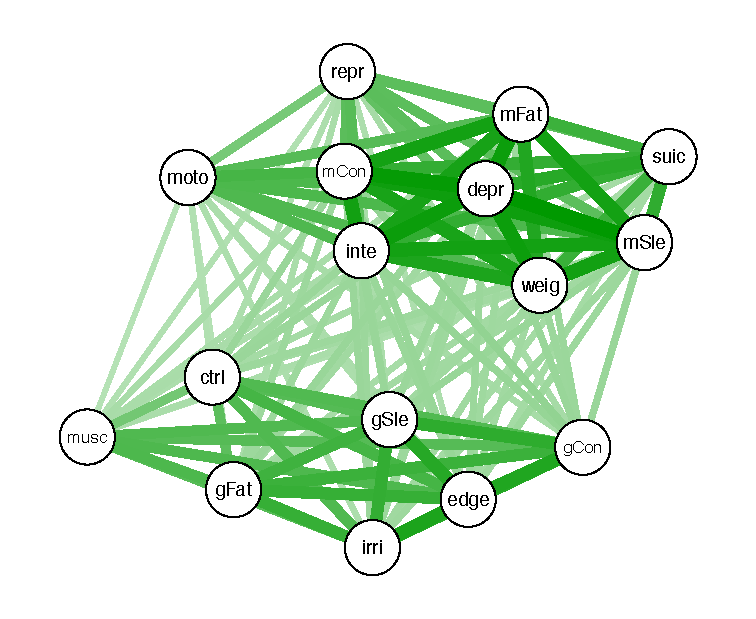
\includegraphics[scale=.6]{pics/scorrdepr}.}\only<2>{The $\hat J$ matrix:\\[.3cm]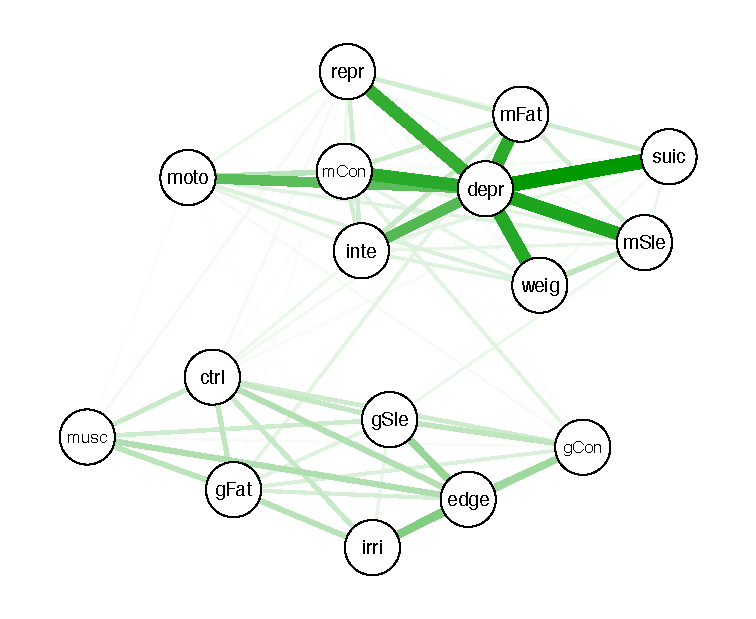
\includegraphics[scale=.6]{pics/Jdepr}}	
\end{center}
\vspace{-.6cm}
\only<1>{{\footnotesize Borsboom and Cramer, Network analysis: an integrative approach to the\\[-.2cm] structure of psychopathology, Annual review of clinical psychology, 9 (2013). }}
\only<2>{{\footnotesize Borsboom and Cramer report a similar picture obtained after asking 12 Dutch\\[-.2cm] clinicians for causal relationships!}}
\end{frame}

\begin{frame}{Testing $H_0: J\geq 0$}
	\begin{alertblock}{Split Likelihood Ratio test}
		Randomly split the data matrix into $X_0,X_1$. \\[.3cm]
		Let $\hat h_1, \hat J_1$ the unrestricted maxima for the Ising model under $X_1$. \\[.3cm]
		Compute the likelihood function $\cL(h,J;X_0)$ and its constrained maximum $\hat h_0$, $\hat J_0$.\\[.3cm]
		We reject the null if $$U_n \;:=\;\frac{\cL(\hat h_1,\hat J_1;X_0)}{\cL(\hat h_0,\hat J_0;X_0)}\;> \;\frac{1}{\alpha}.$$
		Theorem: The split LRT controls the type I error at level $\alpha$, i.e. $\sup_{h,J\geq 0} \P_{\theta_0} (U_n>1/\alpha)\leq \alpha.$
	\end{alertblock}

\end{frame}

%
%\begin{frame}{US Senators voting network}
%	\centering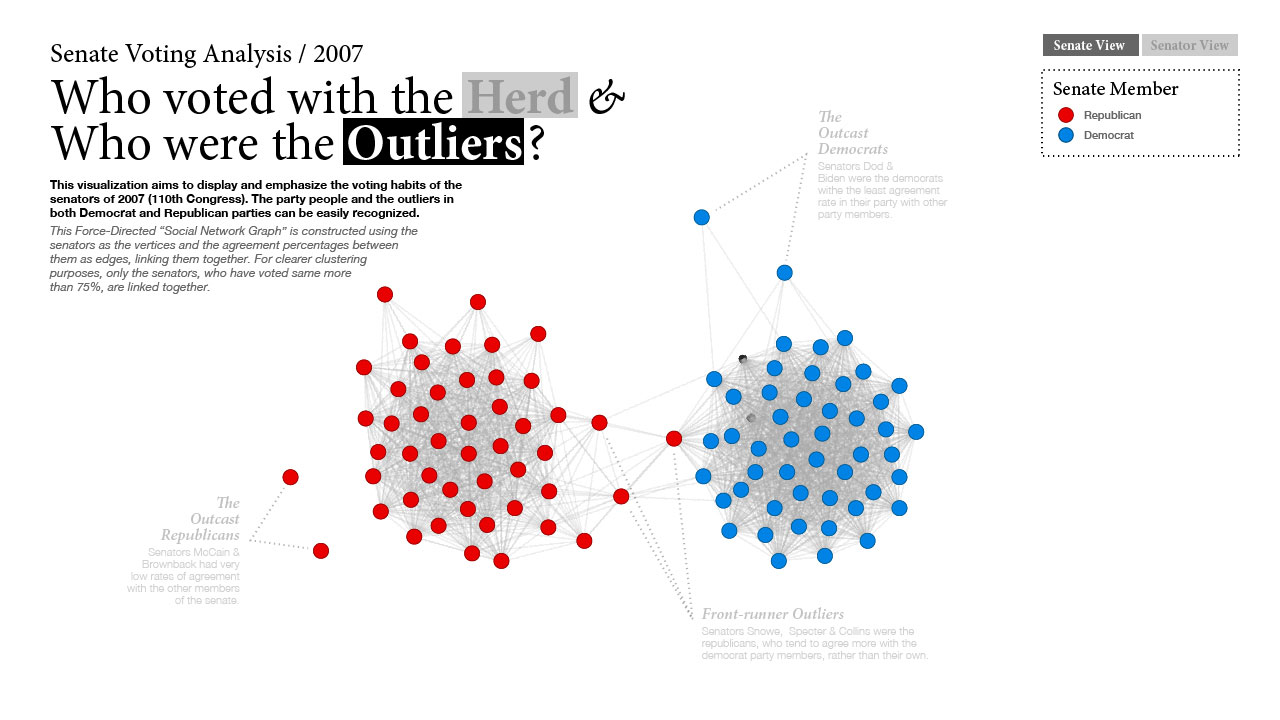
\includegraphics[scale=.28]{pics/ussenate.jpg}
%\end{frame}
%



\end{document}
